\documentclass[a4paper,11pt]{report}
\usepackage{float}
\usepackage[T1]{fontenc}
\usepackage[utf8]{inputenc}
\usepackage{lmodern}
\usepackage{hyperref}
\usepackage[english]{babel}
\usepackage{graphicx}
\usepackage{amsmath}
\usepackage{listings} % package for listing parts of code
\usepackage{cleveref}
\renewcommand*\footnoterule{}

\makeatletter
\renewcommand{\@chapapp}{}% Not necessary...
\newenvironment{chapquote}[2][2em]
{\setlength{\@tempdima}{#1}%
\def\chapquote@author{#2}%
\parshape 1 \@tempdima \dimexpr\textwidth-2\@tempdima\relax%
\itshape}
{\par\normalfont\hfill--\ \chapquote@author\hspace*{\@tempdima}\par\bigskip}
\makeatother


% Book's title and subtitle
\title{\Huge \textbf{High Performance Computing with Python} \vspace{4mm} \\ \huge Final Report}
% Author
% \author{\textsc{First-name Last-name}\footnote{email address}}
\author{\textsc{Jonas Bürgel} \\ \vspace{3mm}\text{5500163}  \\
\vspace{3mm}\text{buergelj@tf.uni-freiburg.de}}


\begin{document}

    \makeatletter
    \begin{titlepage}
        \begin{center}
            
\includegraphics[width=0.5\linewidth]{logos/Uni_Logo-Grundversion_E1_A4_CMYK.eps}\\[4ex]
            {\huge \bfseries  \@title }\\[2ex]
            {\LARGE  \@author}\\[30ex]
            {\large \@date}
        \end{center}
    \end{titlepage}
    \makeatother
    \thispagestyle{empty}
    \newpage



    \tableofcontents


    \chapter{Introduction}

    \chapter{Methods}\label{ch:methods}
This chapter aims to explain fundamentals, used in the experiments.
The focus is on the \textit{probability density function}, \textit{Boltzmann transport equation} and \textit{Lattice Boltzmann scheme}.
The combination of those principles allows simulating fluids in the experiments.
All information in this article is from the lecture of the corresponding course under Prof. Greiner at the University of Freiburg \cite{lecture}.


\section{Probability Density Function (PDF)}\label{sec:probability-density-function-(pdf)}
The Probability Density Function (PDF) is a concept that describes the probability of finding a particle at a certain position.
In theory, the simulation would need to track the individual trajectories of every particle in phase space.
This would require solving a very large number of equations.
Because solving these equations would be too costly, only the averages over the volumes in the phase space are taken using the PDF\@.
Therefore, the PDF, denoted as \(f(\mathbf r_i,\mathbf v_i,t)\), represents the probability density of finding a particle at a certain position \(\mathbf{r_i}\) and velocity \(\mathbf{v_i}\) at a given time \(t\).


\section{Boltzmann Transport Equation (BTE)}
The Boltzmann transport equation formulates the evolution of motion of the PDF over time.
It consists of two parts.
The first part is \textit{streaming} and resembles only the free movement of particles.
The second part is called \textit{collision} and deals with the interaction between particles while moving.
The whole Boltzmann Transport Equation is denoted as
\begin{equation}
    \frac{\partial f\left(\mathbf{r},\mathbf{v},t\right)}{\partial t}+\mathbf{v}\nabla_{\mathbf{r}} f\left(\mathbf{r},\mathbf{v},t\right)
    +\mathbf{a}\nabla_{\mathbf{v}} f\left(\mathbf{r},\mathbf{v},t\right)=C(f)
    \cdot
    \label{eq:bte}
\end{equation}

\subsection{Streaming}\label{subsec:streaming}
The l.h.s.\ of \cref{eq:bte} denotes the streaming part.
The streaming describes the free movement of the densities at a certain velocity.
In the context of this project, movement may happen in 2d space in 9 directions, similar to a queen in chess.
Further information is in \cref{sec:lattice-bolzmann-scheme}.

\subsection{Collision}\label{subsec:collision}
Only applying streaming resembles a 0\% probability of collision between particles, which is not realistic.
To account for collisions, an additional term is introduced at the r.h.s. of \cref{eq:bte} to represent the collision process that occurs at each time step.
In reality, collisions between particles result in an almost instantaneous exchange of energy and momentum.
However, these collisions occur in extremely short time intervals on the order of femtoseconds (\(10^{-15}\) seconds), making it impractical to measure them directly in the model.
Therefore, the collision process is approximated as an instantaneous process.
Because of this instantaneous, it cannot be represented as a differential equation, which normally describes continuous changes.
Instead, a probabilistic approach is taken to describe the effects of collisions.
\newline

The collision part of the Boltzmann transport equation was introduced on the r.h.s.\ in \cref{eq:bte}.
To simplify this collision term, a relaxation time approximation is commonly used.
This approximation assumes that the probability density function (PDF) \(f\left(\mathbf{r},\mathbf{v},t\right)\) relaxes towards a local equilibrium distribution, denoted as \(f^{eq}\left(\mathbf{r},\mathbf{v},t\right)\).
By interpreting the streaming term as the total time derivative of the PDF, the BTE can be reformulated as follows:

\begin{equation}
    \frac{d}{dt} f\left(\mathbf{r},\mathbf{v},t\right) = -\frac{ f\left(\mathbf{r},\mathbf{v},t\right)- f^{eq}\left(\mathbf{r},\mathbf{v},t\right)}{\tau}
    \cdot
    \label{eq:bgk}
\end{equation}

The included equilibirum function can be denoted as
\begin{equation}
    f_i^{eq}(\rho(\mathbf{r}),\mathbf{u}(\mathbf{r}))
    =w_i\rho(\mathbf{r})
    \left[
        1+3\mathbf{c}_i\cdot\mathbf{u}(\mathbf{r})
        +\frac{9}{2}\left(\mathbf{c}_i\cdot\mathbf{u}(\mathbf{r})\right)^2
        -\frac{3}{2}|\mathbf{u}(\mathbf{r})|^2
        \right]
    \cdot
    \label{eq:feq}
\end{equation}

The equilibrium function introduces some additional quantities, namely the density \(\rho(\mathbf{r})\), velocity \(\mathbf{u}(\mathbf{r})\) and \(w_i\).
\(w_i\) is defined for a D2Q9 lattice as seen in~\cref{eq:w}.
The other two quantities can be calculated using the following formulas
\begin{equation}
    w_i = \left(\dfrac{4}{9},
    \dfrac{1}{9}, \dfrac{1}{9}, \dfrac{1}{9}, \dfrac{1}{9},
    \dfrac{1}{36}, \dfrac{1}{36}, \dfrac{1}{36}, \dfrac{1}{36}\right)
    \label{eq:w}
\end{equation}
\begin{equation}
    \rho(\mathbf{r})=\sum_i f_i
    \label{eq:rho}
\end{equation}
\begin{equation}
    \mathbf{u}(\mathbf{r})=
    \frac{1}{\rho(\mathbf{r})}\sum_i \mathbf{c}_i f_i(\mathbf{r}) \cdot
    \label{eq:u}
\end{equation}


\section{Lattice Bolzmann Scheme}\label{sec:lattice-bolzmann-scheme}

In order to discretize the Boltzmann Transport Equation (BTE), it is necessary to incorporate both velocity and position space into the discrete scheme representation.
An effective approach involves utilizing a 2D grid, as illustrated in \cref{fig:bte-scheme}.
The grid represents the position space as coordinates of the x and y coordinates.

\begin{figure}[H]
    \begin{center}
        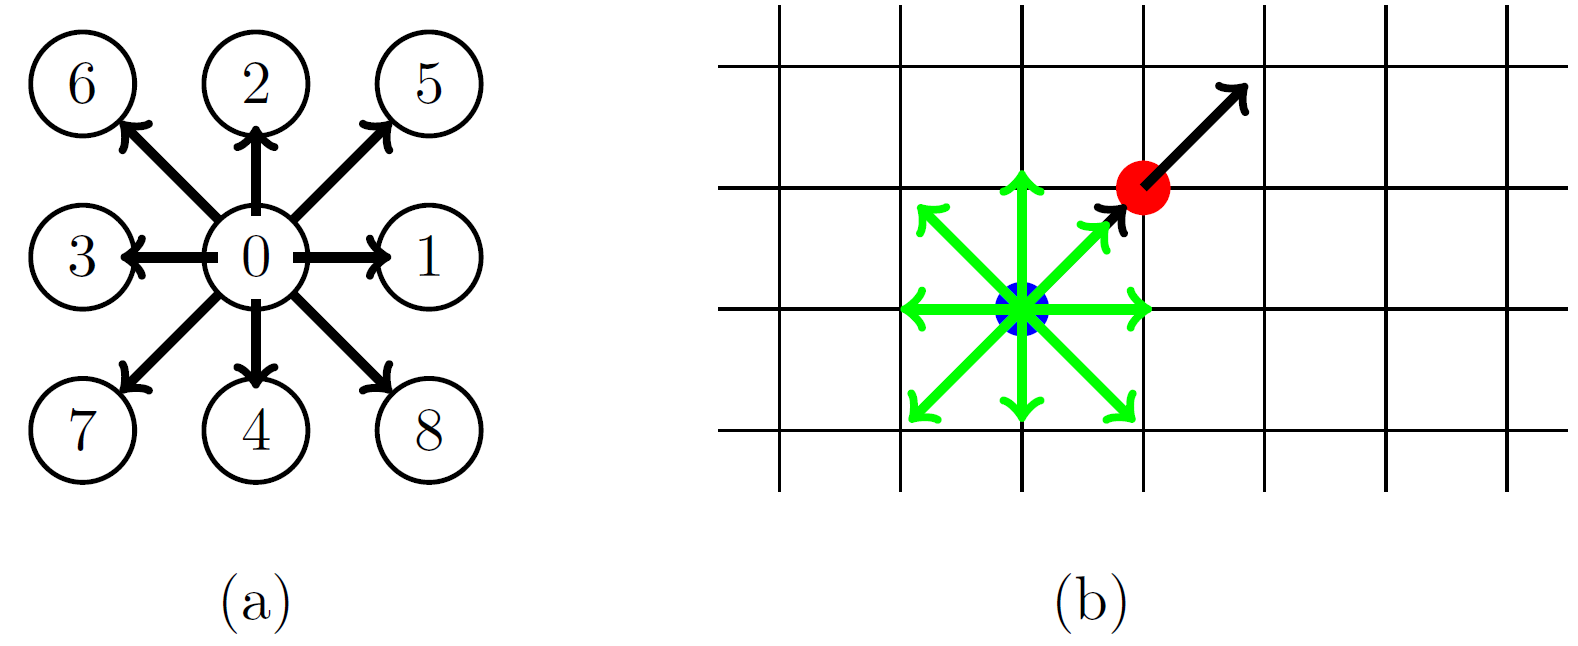
\includegraphics[width=10cm]{logos/Gitter_LBM.png}
        \caption[Visualization of the underlying grid including labled directions.]{
            Visualization of the underlying grid including labled directions. \\
            (a) directions with given labels \\
            (b) streaming example of one particle
        }
        \label{fig:bte-scheme}
    \end{center}
\end{figure}

Each position holds a probability density value, resembled by the value at that point.
The velocities are included when introducing a third dimension, that separates the different streaming directions.
To get the probability density function back, only the sum of all different directions in one point is needed.
The probability density function can be reconstructed by simply summing the values for all different directions at a given point.
\newline

The streaming, as explained in \cref{subsec:streaming}, is applied by moving the values of the points in one of 9 directions in their respective dimension.
The collision process can be implemented by employing the functions described in \cref{subsec:collision}.
During collisions, densities may be transferred between different dimensions within the scheme.


\section{Reynolds Number}\label{sec:reynolds-number}
The Reynolds Number is used to compare results of different simulations.
The same Reynolds Number indicates, that the simulations are comparable.
It is calculated by the following formula where $L$ is the size of one simulation dimension, $u$ the velocity or speed and $\nu$ the viscosity of the simulated fluid

\begin{equation*}
    \begin{gathered}
        u = avg(\sqrt{\mathbf u_x^2 * \mathbf u_y^2}) \\
        Re = \frac{L u}{\nu} \cdot
    \end{gathered}
\end{equation*}


    \chapter{Implementation}


\section{Setup}
This section deals with the topic of setting up this project and to navigate through it.
It is intended to readers who want to run the experiments themselves or help to dig into the exact implementations.

\subsection{Environment}
This project was developed using pyenv and pip.
Pyenv was selected due to its ability to create a virtual Python environment while still utilizing pip as the native package manager, distinguishing it from alternatives like anaconda.
\newline

The project's requirements are outlined in the requirements.txt file, and the desired Python version is specified in the .python-version file, generated by pyenv.
To install the requirements, execute the following commands in the project's top directory within a Bash environment:

\begin{center}
    \begin{lstlisting}[language=bash]
#!/bin/bash
pyenv install 3.11
pyenv local 3.11
source venv/bin/activate
pip install -r requirements.txt
    \end{lstlisting}
\end{center}

\subsection{Code Structure}
The project consists of three primary folders: \textit{src/shared}, \textit{src/experiments}, and \textit{tests}.
The \textit{tests} folder contains code dedicated to programmatic validation of the implementations, primarily comprising unit tests.
The \textit{src/shared} folder contains code that is shared among all experiments conducted in the project.
This includes implementations for streaming and collision in the lib file, among others.
Lastly, the \textit{src/experiments} folder contains experiment-specific code, including plotting functionalities tailored to each experiment.


\section{Probability Density Function}
The probability density function is modelled as a \textit{numpy} array with 3 dimensions, namely: channels, x-direction and y-direction in this order.
While the number of channels allways has to be exactly 9, the x and y dimensions may vary in size and are independent of each other.
These constraints to the probability density function are assumed by all implemented functions and have to hold at all time.
\newline

The Probability density function follows the scheme described in \cref{sec:lattice-bolzmann-scheme}.
While the grid in \cref{fig:bte-scheme} resembles the second and third dimension of the PDF, the channels can be imagined as a third dimension on the grid.
Each channel resembles one direction of moving as shown in the left part of \cref{fig:bte-scheme}.
The indices of the channels are in line with the indices of the arrows in the graphic.


\section{Main Routine}\label{sec:main-routine}
The main routine may be seen as a function that is repeated until the experiment is over.
It consists of several operators that stay the same in each experiment.
For some experiments, not all operators are used or for example the \textit{bounce-back} is only applied to certain walls.
\textbf{The order of the operators always stays the same and is crucial for a successive experiment}.
All possible operators are listed below:
\begin{enumerate}
    \item collision - handles colliding particles in the simulation
    \item slide - applies a steady velocity to on side
    \item bounce back - bounces particles back into from certain walls
    \item stream - moves all particles
\end{enumerate}

An interested reader may find the exact implementation in \textit{src/shared/boltzmann.py}.
As it is redundant and maybe not inline with the exact implementation there won't be code examples at this point.
However, it is to mention that all examples follow strictly the formulas explained in \cref{ch:methods}, so there is no special need in doing so.


\section{Parallelization}\label{sec:parallelization}
The last experiment \cref{sec:sliding-lit} utilizes the \textit{mpi4py} package to parallelize its run.
The MPI interface allows spreading the array of the probability density function over several processes.
Each process then determines the result of the main routine (described in \cref{sec:main-routine}) for its subarray.
Afterward, the results are combined by shifting the boundaries of each subarray.
\newline

A right shift for process 4 works as following, if assuming that there are the processes 3, 4 and 5.
Process 4 would receive the right side from process 3 and save it in its left side.
Simultaneously, process 4 would send its right side to process 5.
This is repeated for all processes.
The exact topology of the processes may vary and is determined by MPI itself.

    \chapter{Results}


\section{Shear Wave Decay}
The Shear Wave Decay is a common concept in computational physics to measure the kinematic viscosity of a fluid.
It is set up by creating an initial sinusoidal velocity profile and measuring the decay rate.
The field is set up with a periodic boundary condition on each side, which results in e.g.\ particles moving out of the right to appear back on the left side.
The default parameters for the Shear Wave Decay experiments are shown in \cref{tab:swd-parameters} and used if not stated otherwise.

\begin{table}[ht]
    \centering % used for centering table
    \begin{tabular}{c c}
% centered columns (4 columns)
        \hline\hline %inserts double horizontal lines
        Parameter  & Value \\ [0.5ex] % inserts table heading
        \hline % inserts single horizontal line
        $L_x$      & 100   \\
        $L_y$      & 100   \\
        $\omega$   & 1.0   \\
        $\epsilon$ & 0.01  \\
        $t_{\max}$ & 1000  \\ [1ex] % [1ex] adds vertical space
        \hline %inserts single line
    \end{tabular}
    \caption{Parameters for the Shear Wave Decay} % title of Table
    \label{tab:swd-parameters}
\end{table}

\subsection{Sinusodial Density}
The initial condition is a given by the following equation where $L_x$ resembles the size in x-direction

\begin{equation*}
    \begin{aligned}
        \mathbf{u}(\mathbf{r},0) &= 0 \\
        \rho(\mathbf{r},0) &= \rho_0 + \epsilon \sin \left( \frac{2 \pi x}{L_x} \right) \cdot
    \end{aligned}
\end{equation*}

Because of the initialization the fluid is shaped like a sinusoid wave without any velocity.
It is expected that this wave collapses in itself.
This is due to the fact that the system tries to reach a state of equilibrium where the mass at each position is the same.
Therefore, a flow is created from the higher density area to the lower density area.
This flow continues until the mass at the previous lower density area is so dense, that no further flow is created. %TODO better explaining why it overflows!
It now reached a state similar to the beginning however the dense and low-dense areas swapped which is why the flow will have opposite directions in the next iteration.
This process can be seen in \cref{fig:swd-stream-velocity}. % TODO fix formatting (text-image-text-image)

\begin{figure}[h!]
    \begin{minipage}{0.33\textwidth}
        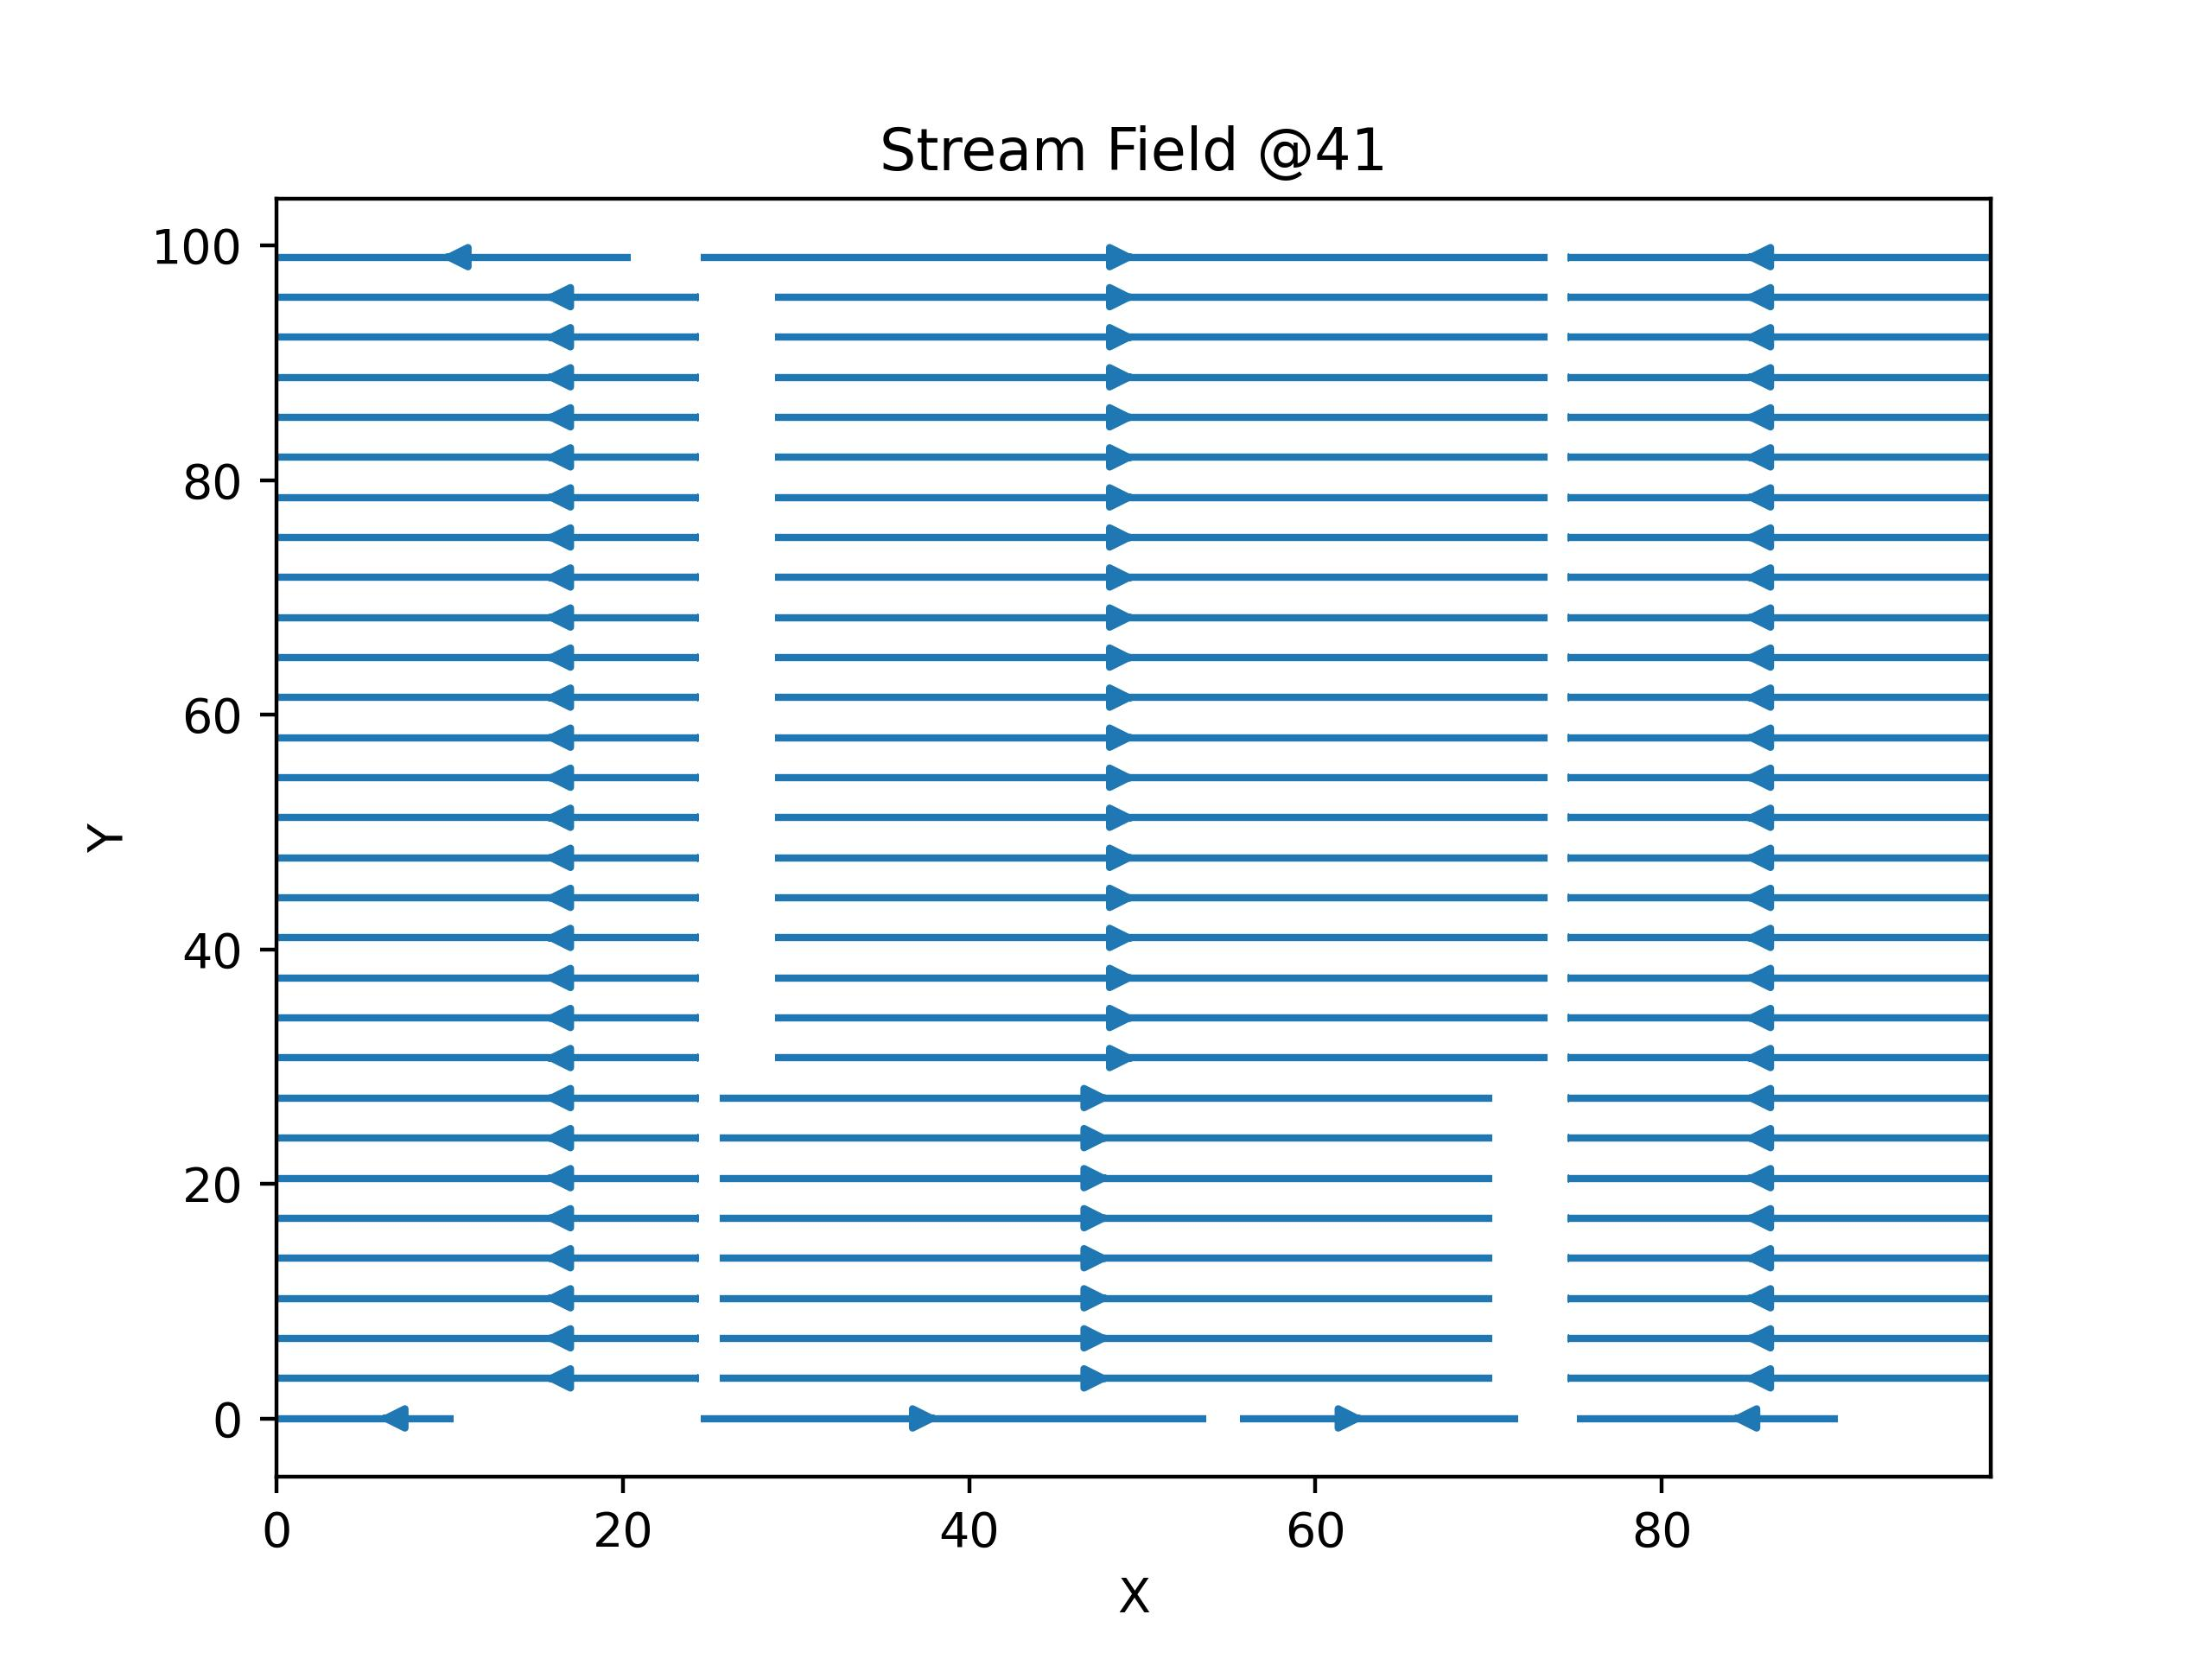
\includegraphics[width=\linewidth]{graphs/ShearWaveDecay/DensityDistribution/stream_field_41}
    \end{minipage}% don't remove this comment - uncomments a new line
    \begin{minipage}{0.33\textwidth}
        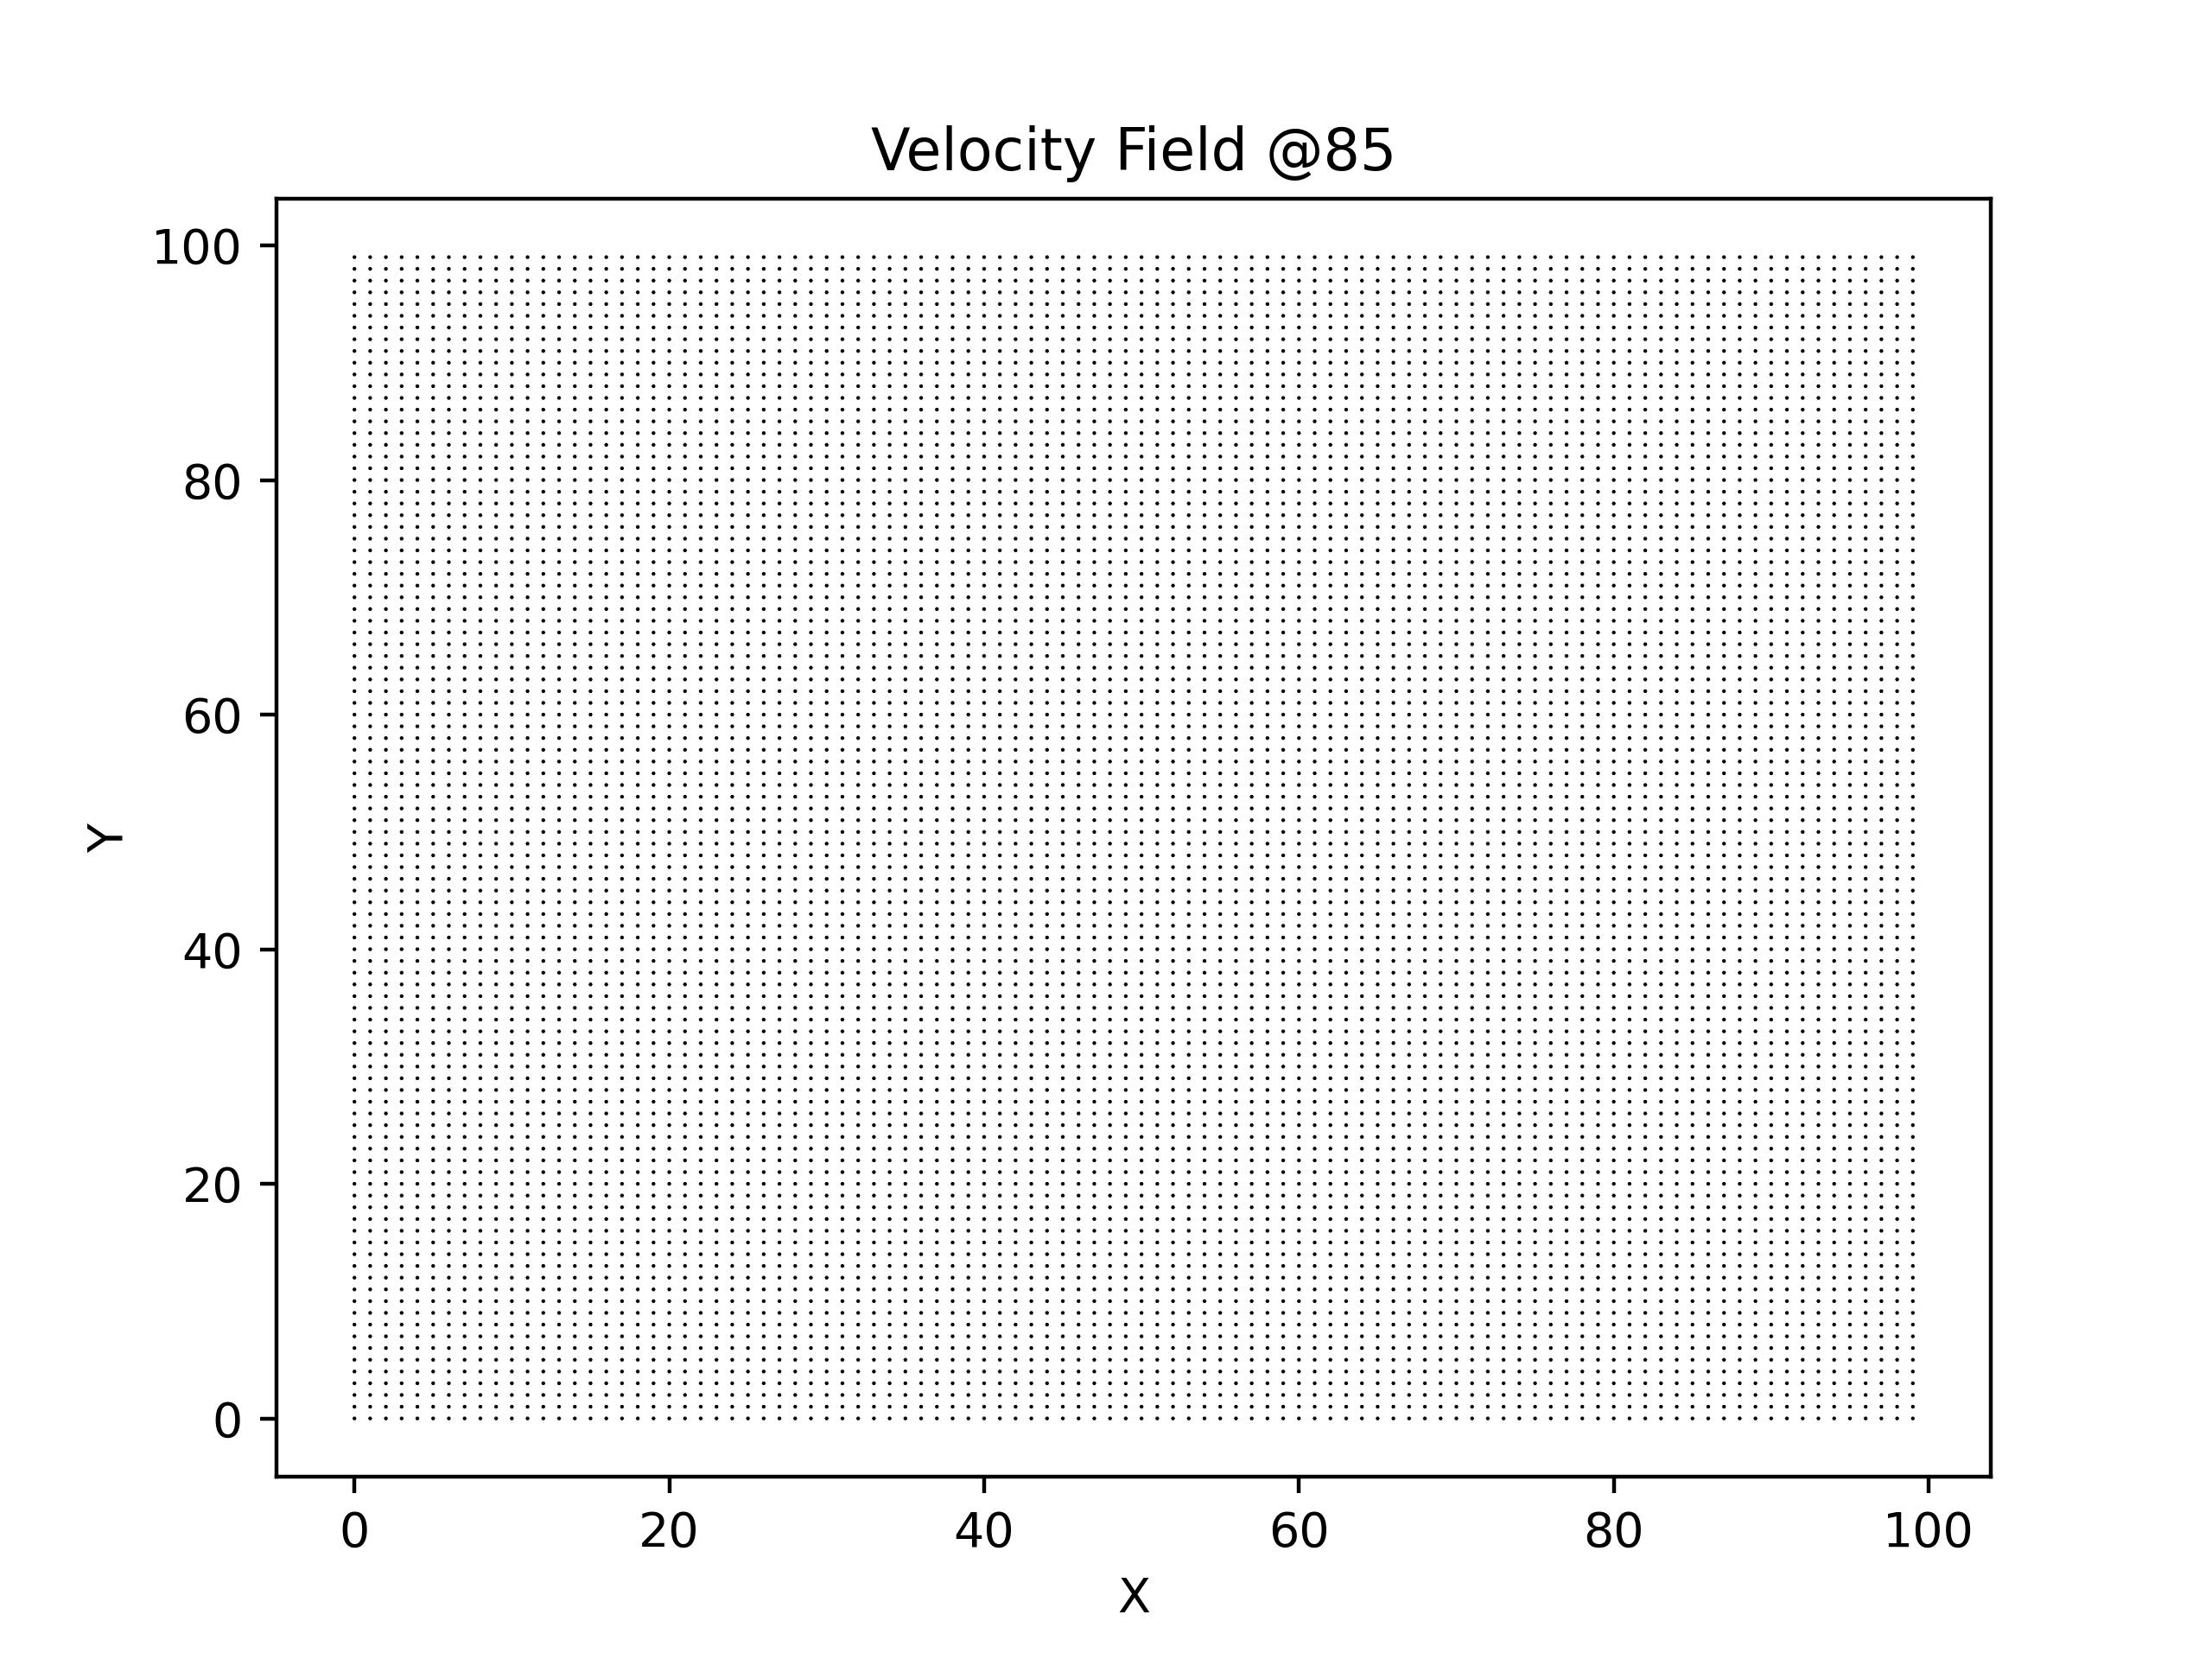
\includegraphics[width=\linewidth]{graphs/ShearWaveDecay/DensityDistribution/velocity_field_85}
    \end{minipage}% don't remove this comment - uncomments a new line
    \begin{minipage}{0.33\textwidth}
        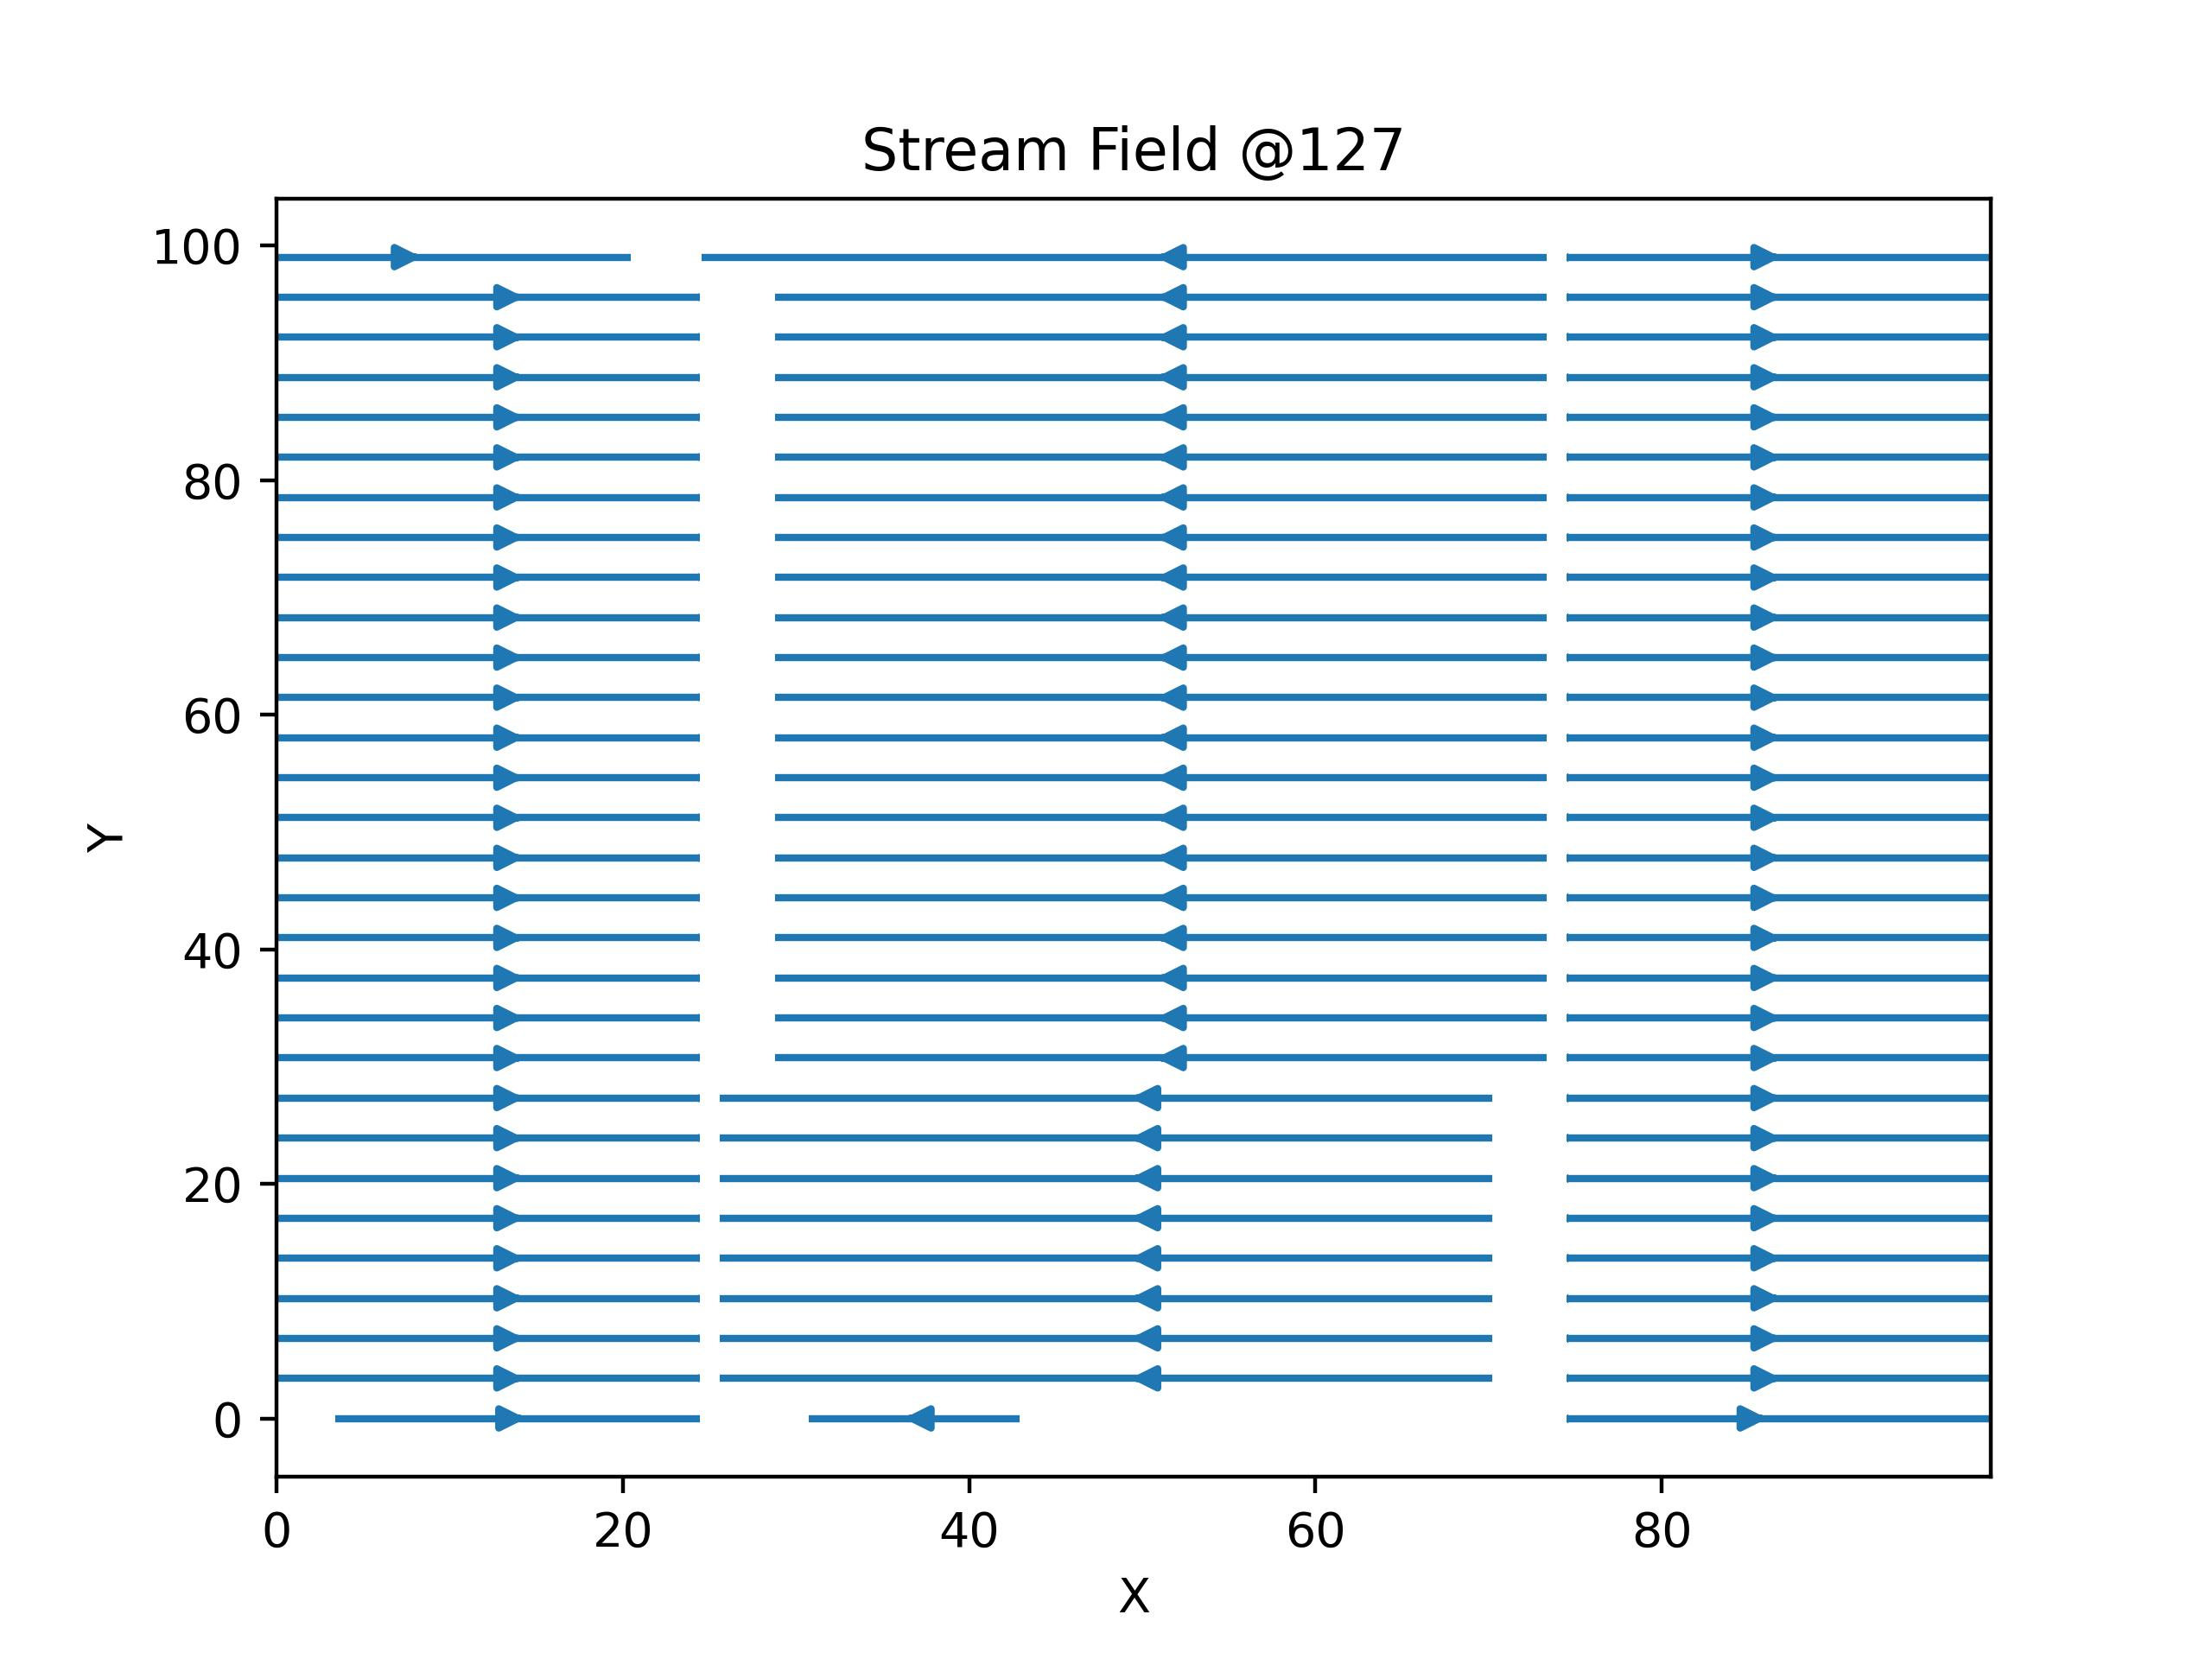
\includegraphics[width=\linewidth]{graphs/ShearWaveDecay/DensityDistribution/stream_field_127}
    \end{minipage}
    \caption{
        Different flow states during the simulation.
        From piling up at step 41 to a steady state at step 85 to the opposite flow at step 127.
    }
    \label{fig:swd-stream-velocity}
\end{figure}

This flow won't hold forever as the newly forming dense areas are always less dense as the once from the previous iteration.
The system tries to reach an equilibrium.
Over time the piles are shallower and shallower until it reaches the desired equilibrium function with the same density at all positions.
The decay is shown through the plots in \cref{fig:swd-decay}.

\begin{center}
    \begin{figure}[h!]
        \begin{minipage}{0.5\textwidth}
            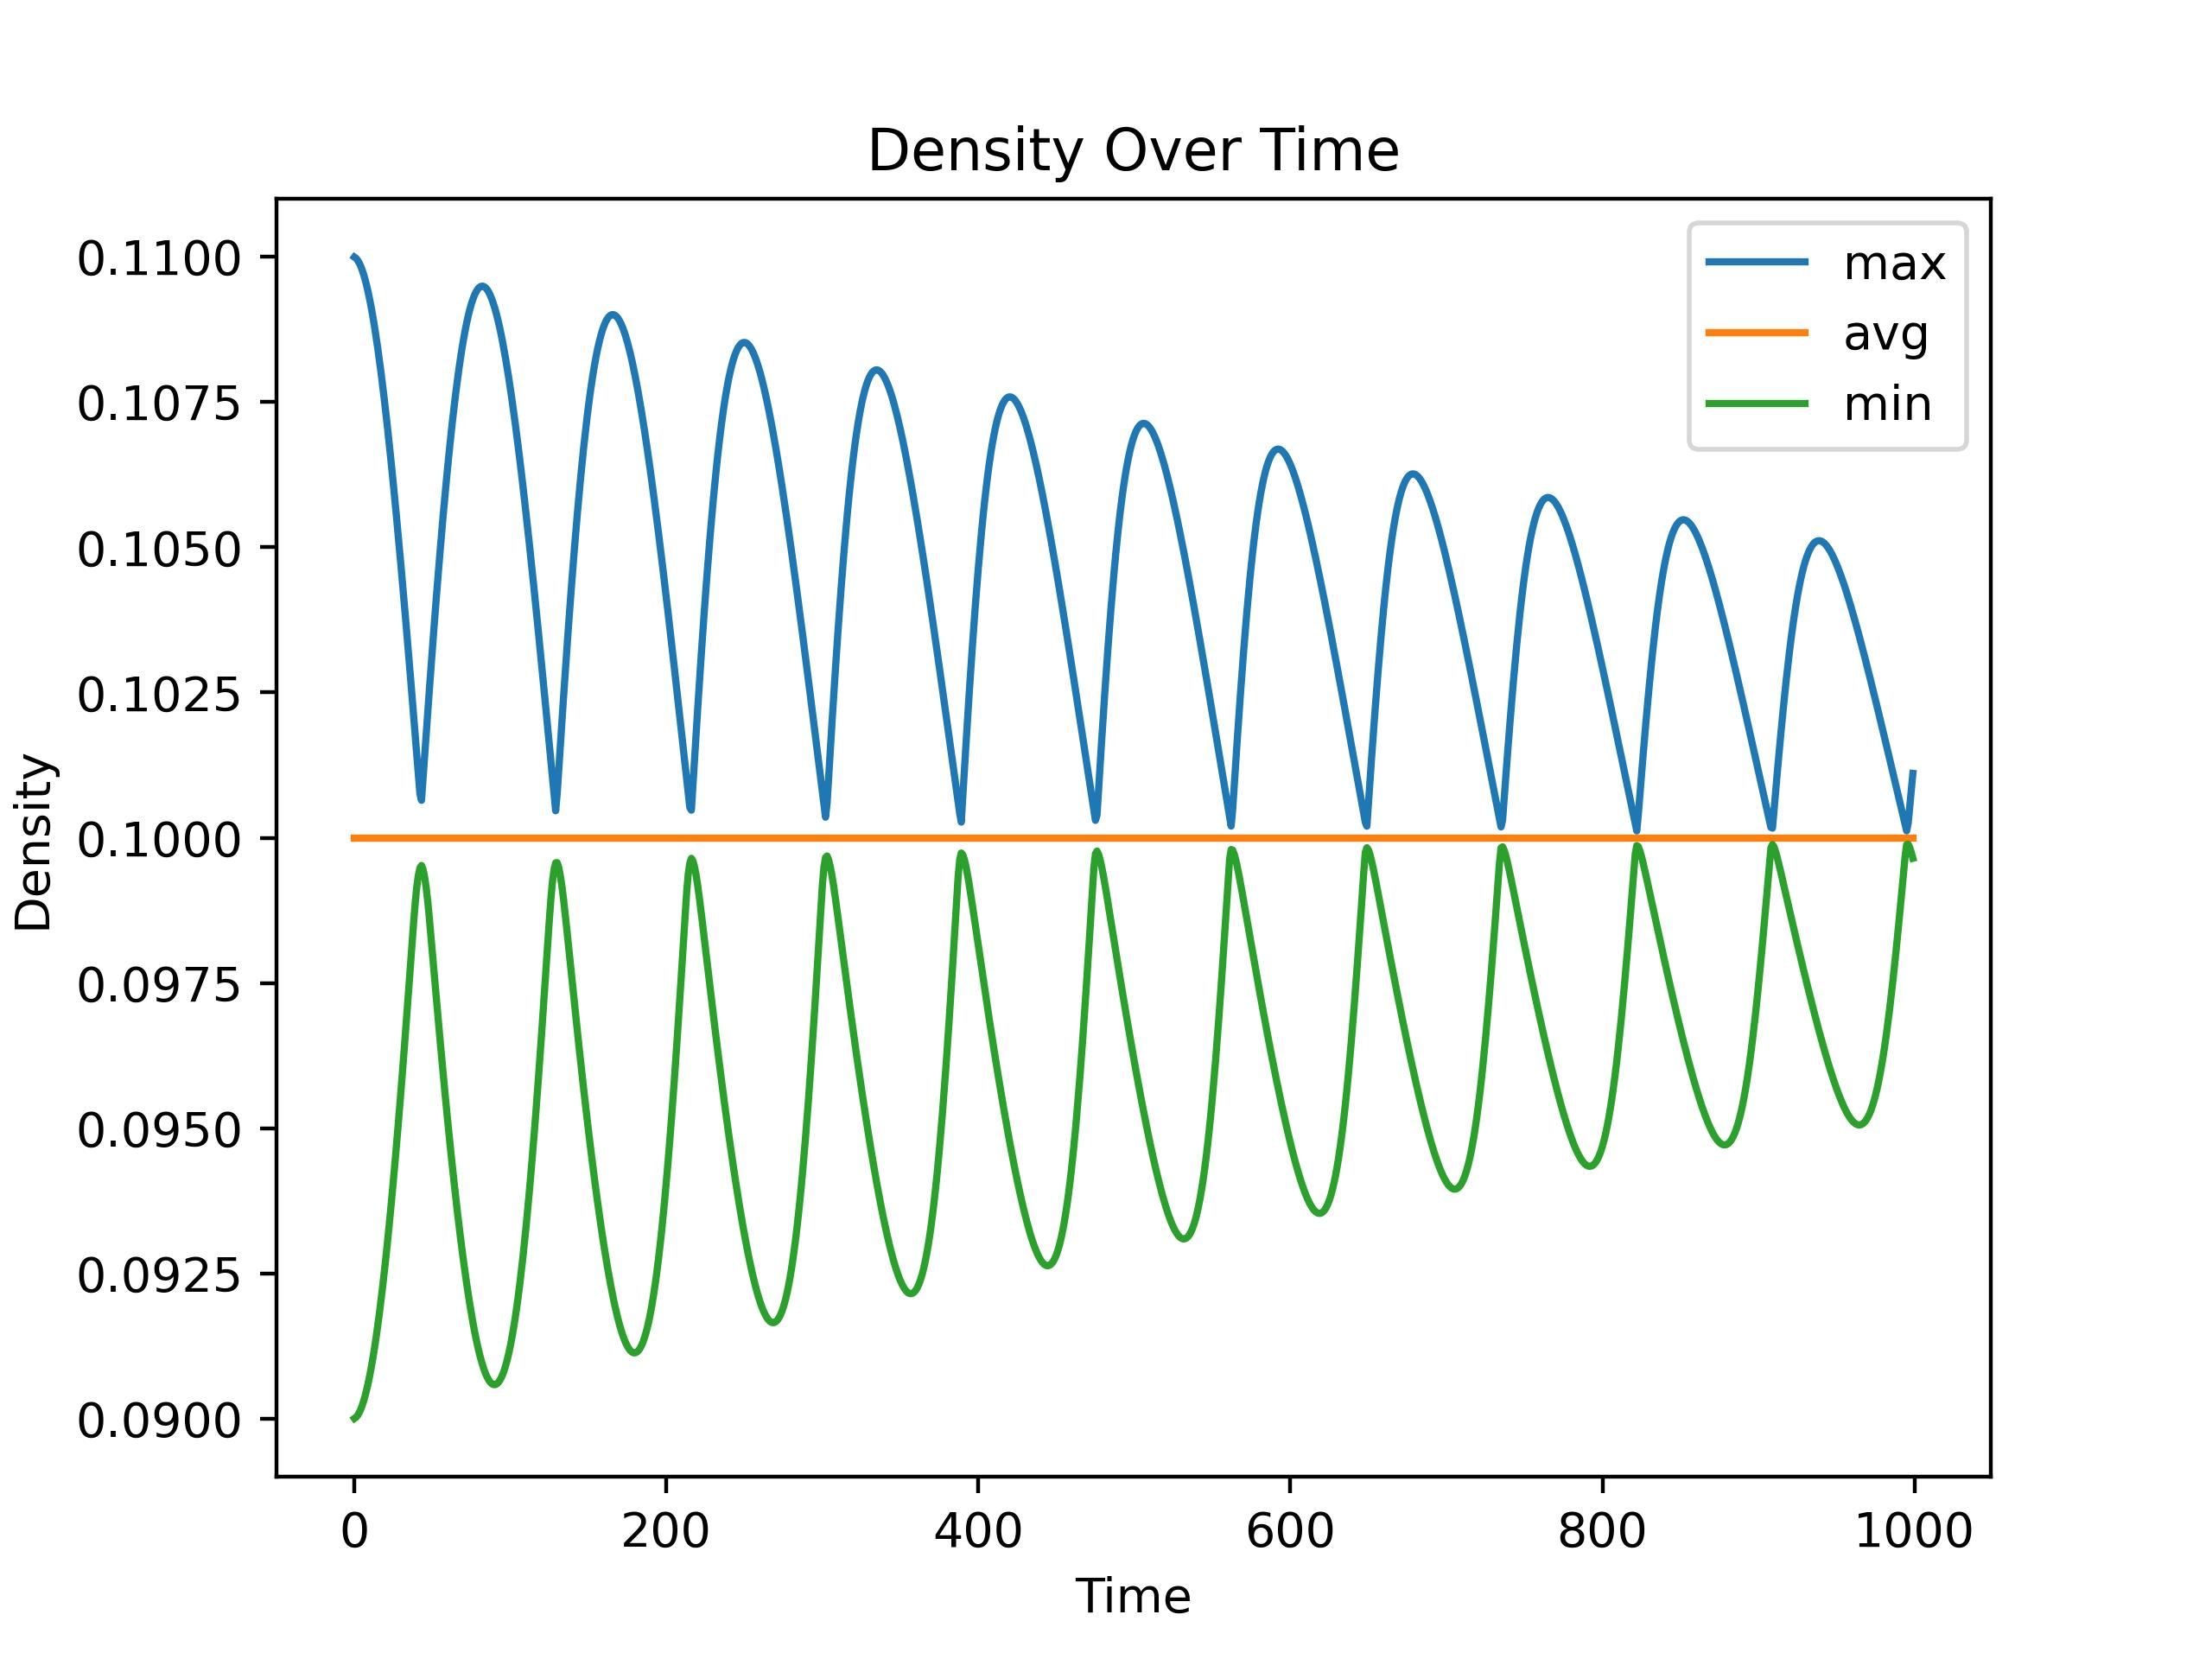
\includegraphics[width=\linewidth]{graphs/ShearWaveDecay/DensityDistribution/density_aggregate_over_time.jpg}
        \end{minipage}% don't remove this comment - uncomments a new line
        \begin{minipage}{0.5\textwidth}
            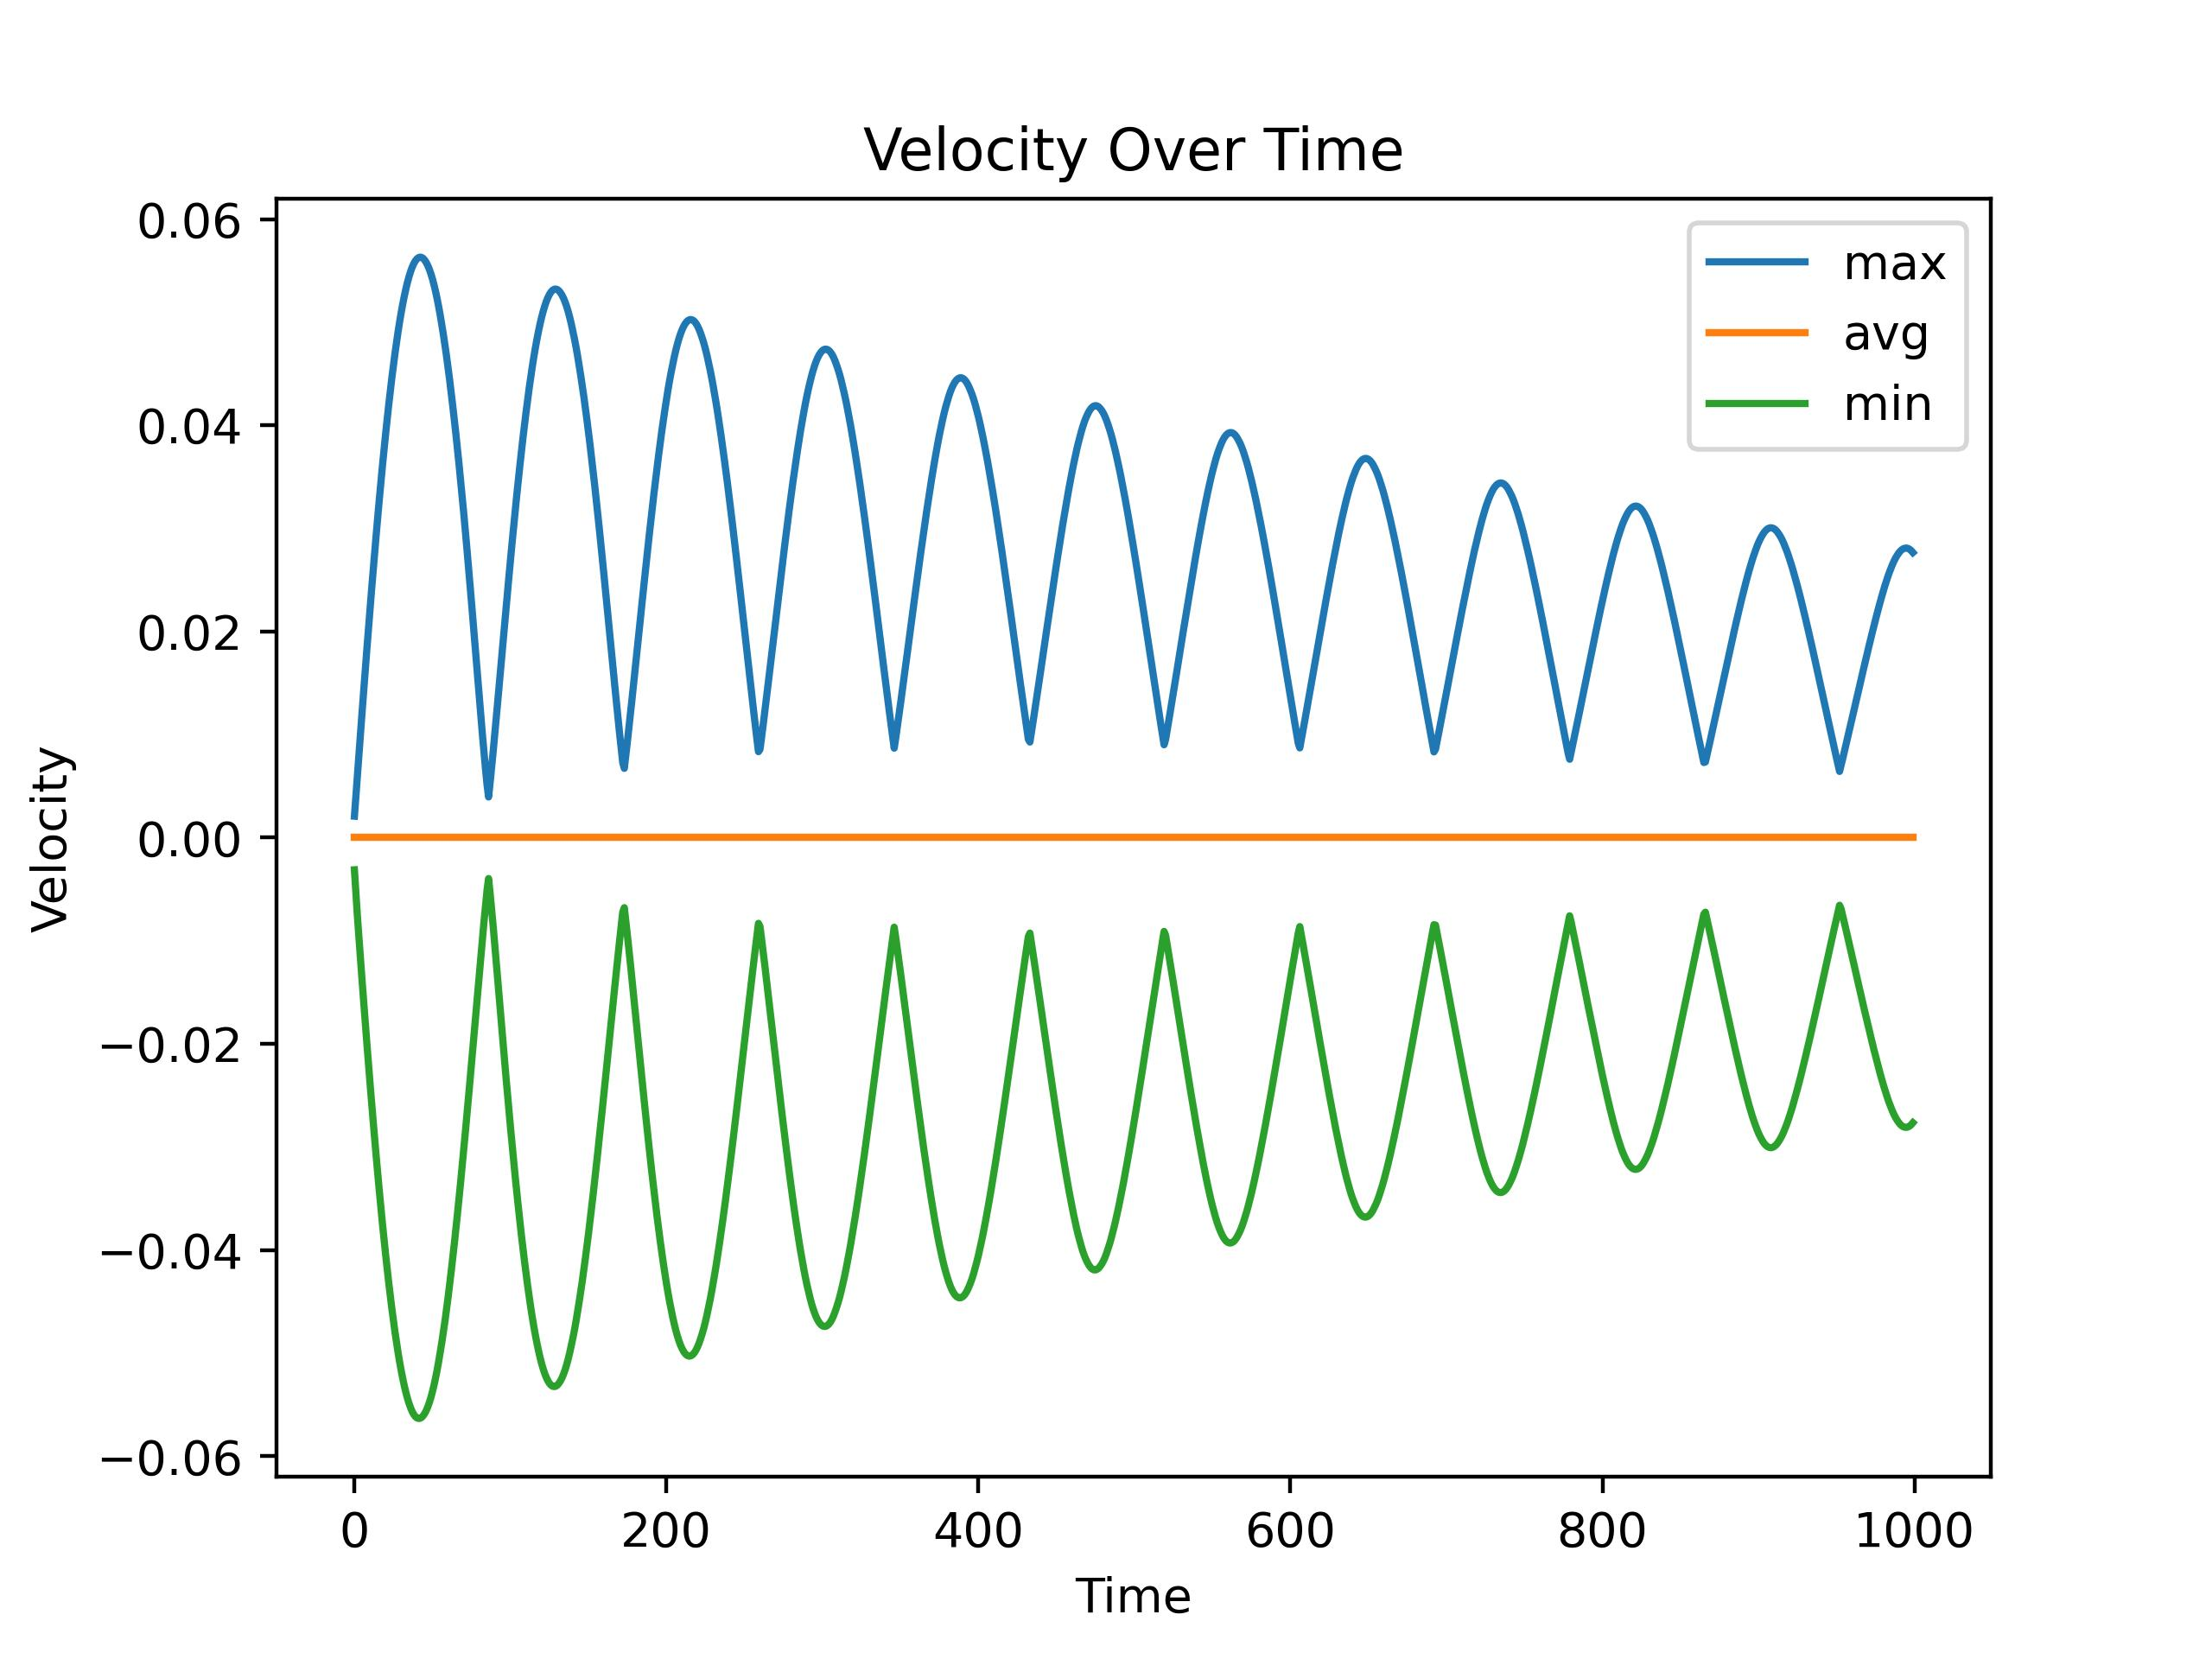
\includegraphics[width=\linewidth]{graphs/ShearWaveDecay/DensityDistribution/velocity_aggregate_over_time.jpg}
        \end{minipage}
        \caption{Decaying density and velocity over time.}
        \label{fig:swd-decay}
    \end{figure}
\end{center}

\subsection{Sinusoidal Velocity}\label{subsec:sinusoidal-velocity}
\textbf{This experiment ran with an epsilon of 0.5 to display the effect more drastically.}
The initial condition is a given by the following equation where $L_y$ resembles the size in y-direction and $\epsilon$ resembles the initial amplitude

\begin{equation*}
    \begin{aligned}
        u_x(\mathbf{r},0) &= \epsilon \sin \left( \frac{2 \pi x}{L_y} \right) \\
        \rho(\mathbf{r},0) &= 1 \cdot
    \end{aligned}
\end{equation*}

Because of the initial condition, the flow varies throughout the field.
The equilibrium state is a state without a clearly directed movement as in the initial condition.
So it is expected that the flow will decrease over time.

\begin{figure}[h!]
    \begin{minipage}{0.33\textwidth}
        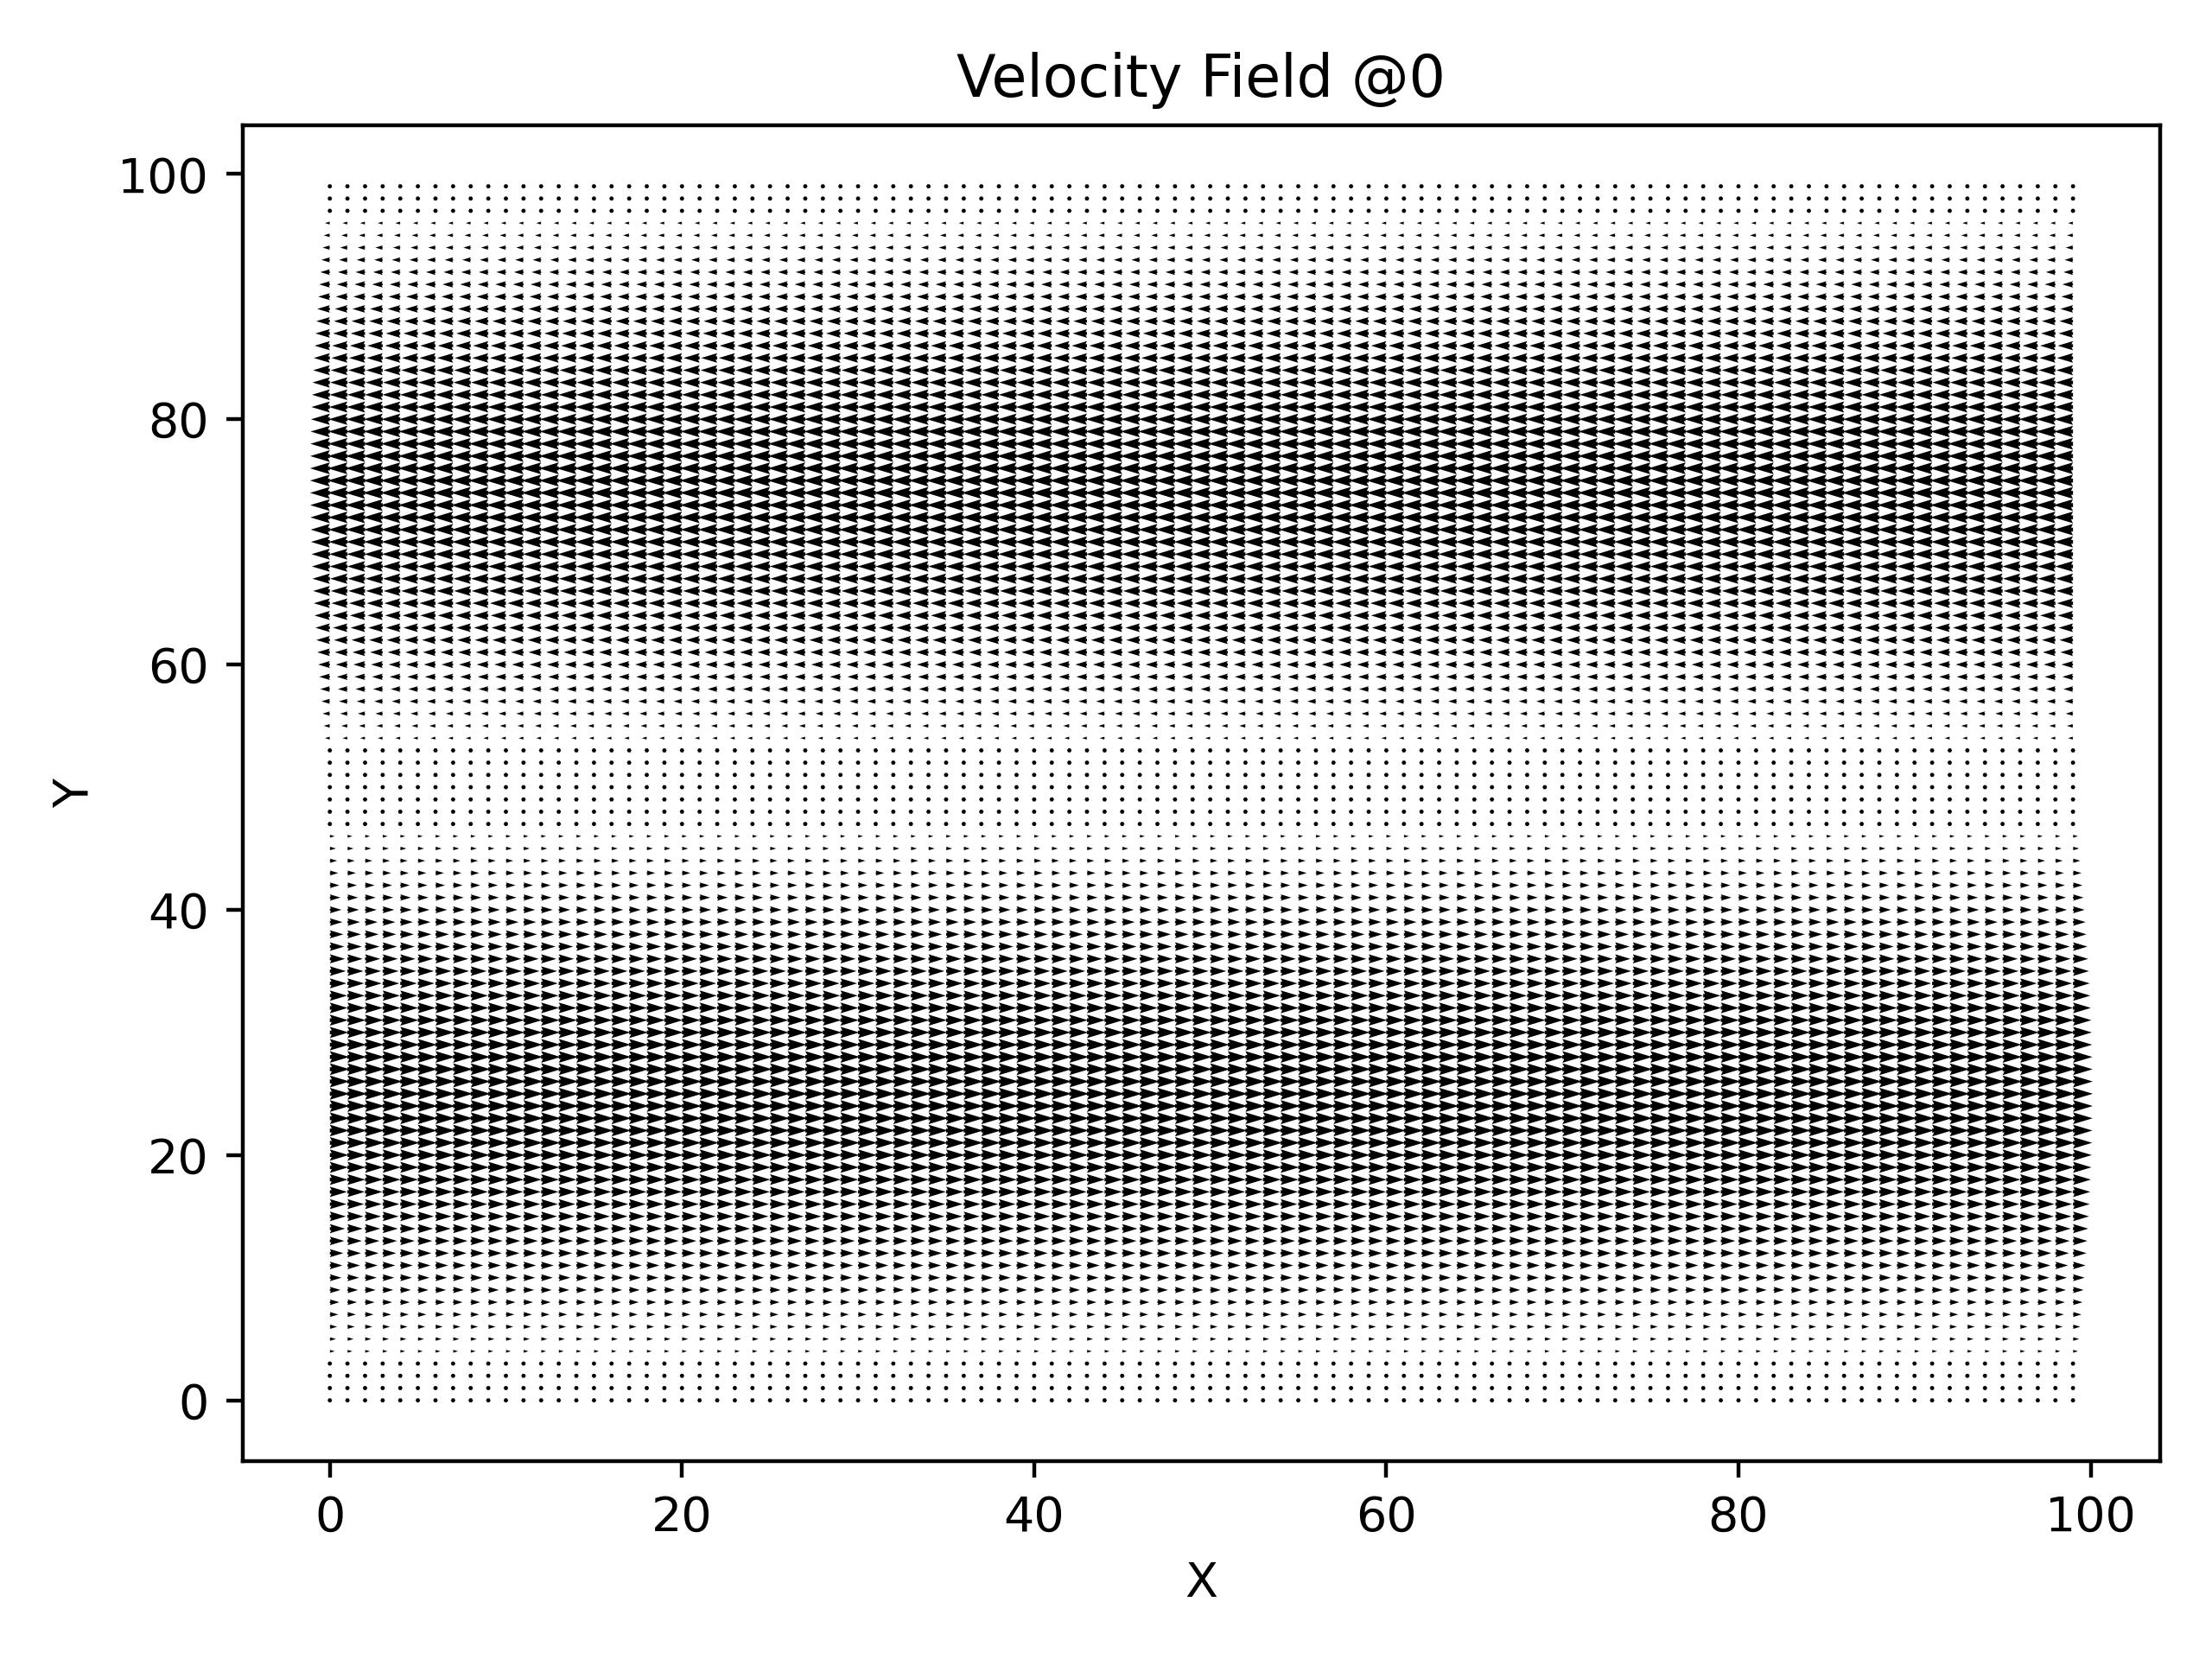
\includegraphics[width=\linewidth]{graphs/ShearWaveDecay/VelocityDistribution/velocity_field_0}
    \end{minipage}% don't remove this comment - uncomments a new line
    \begin{minipage}{0.33\textwidth}
        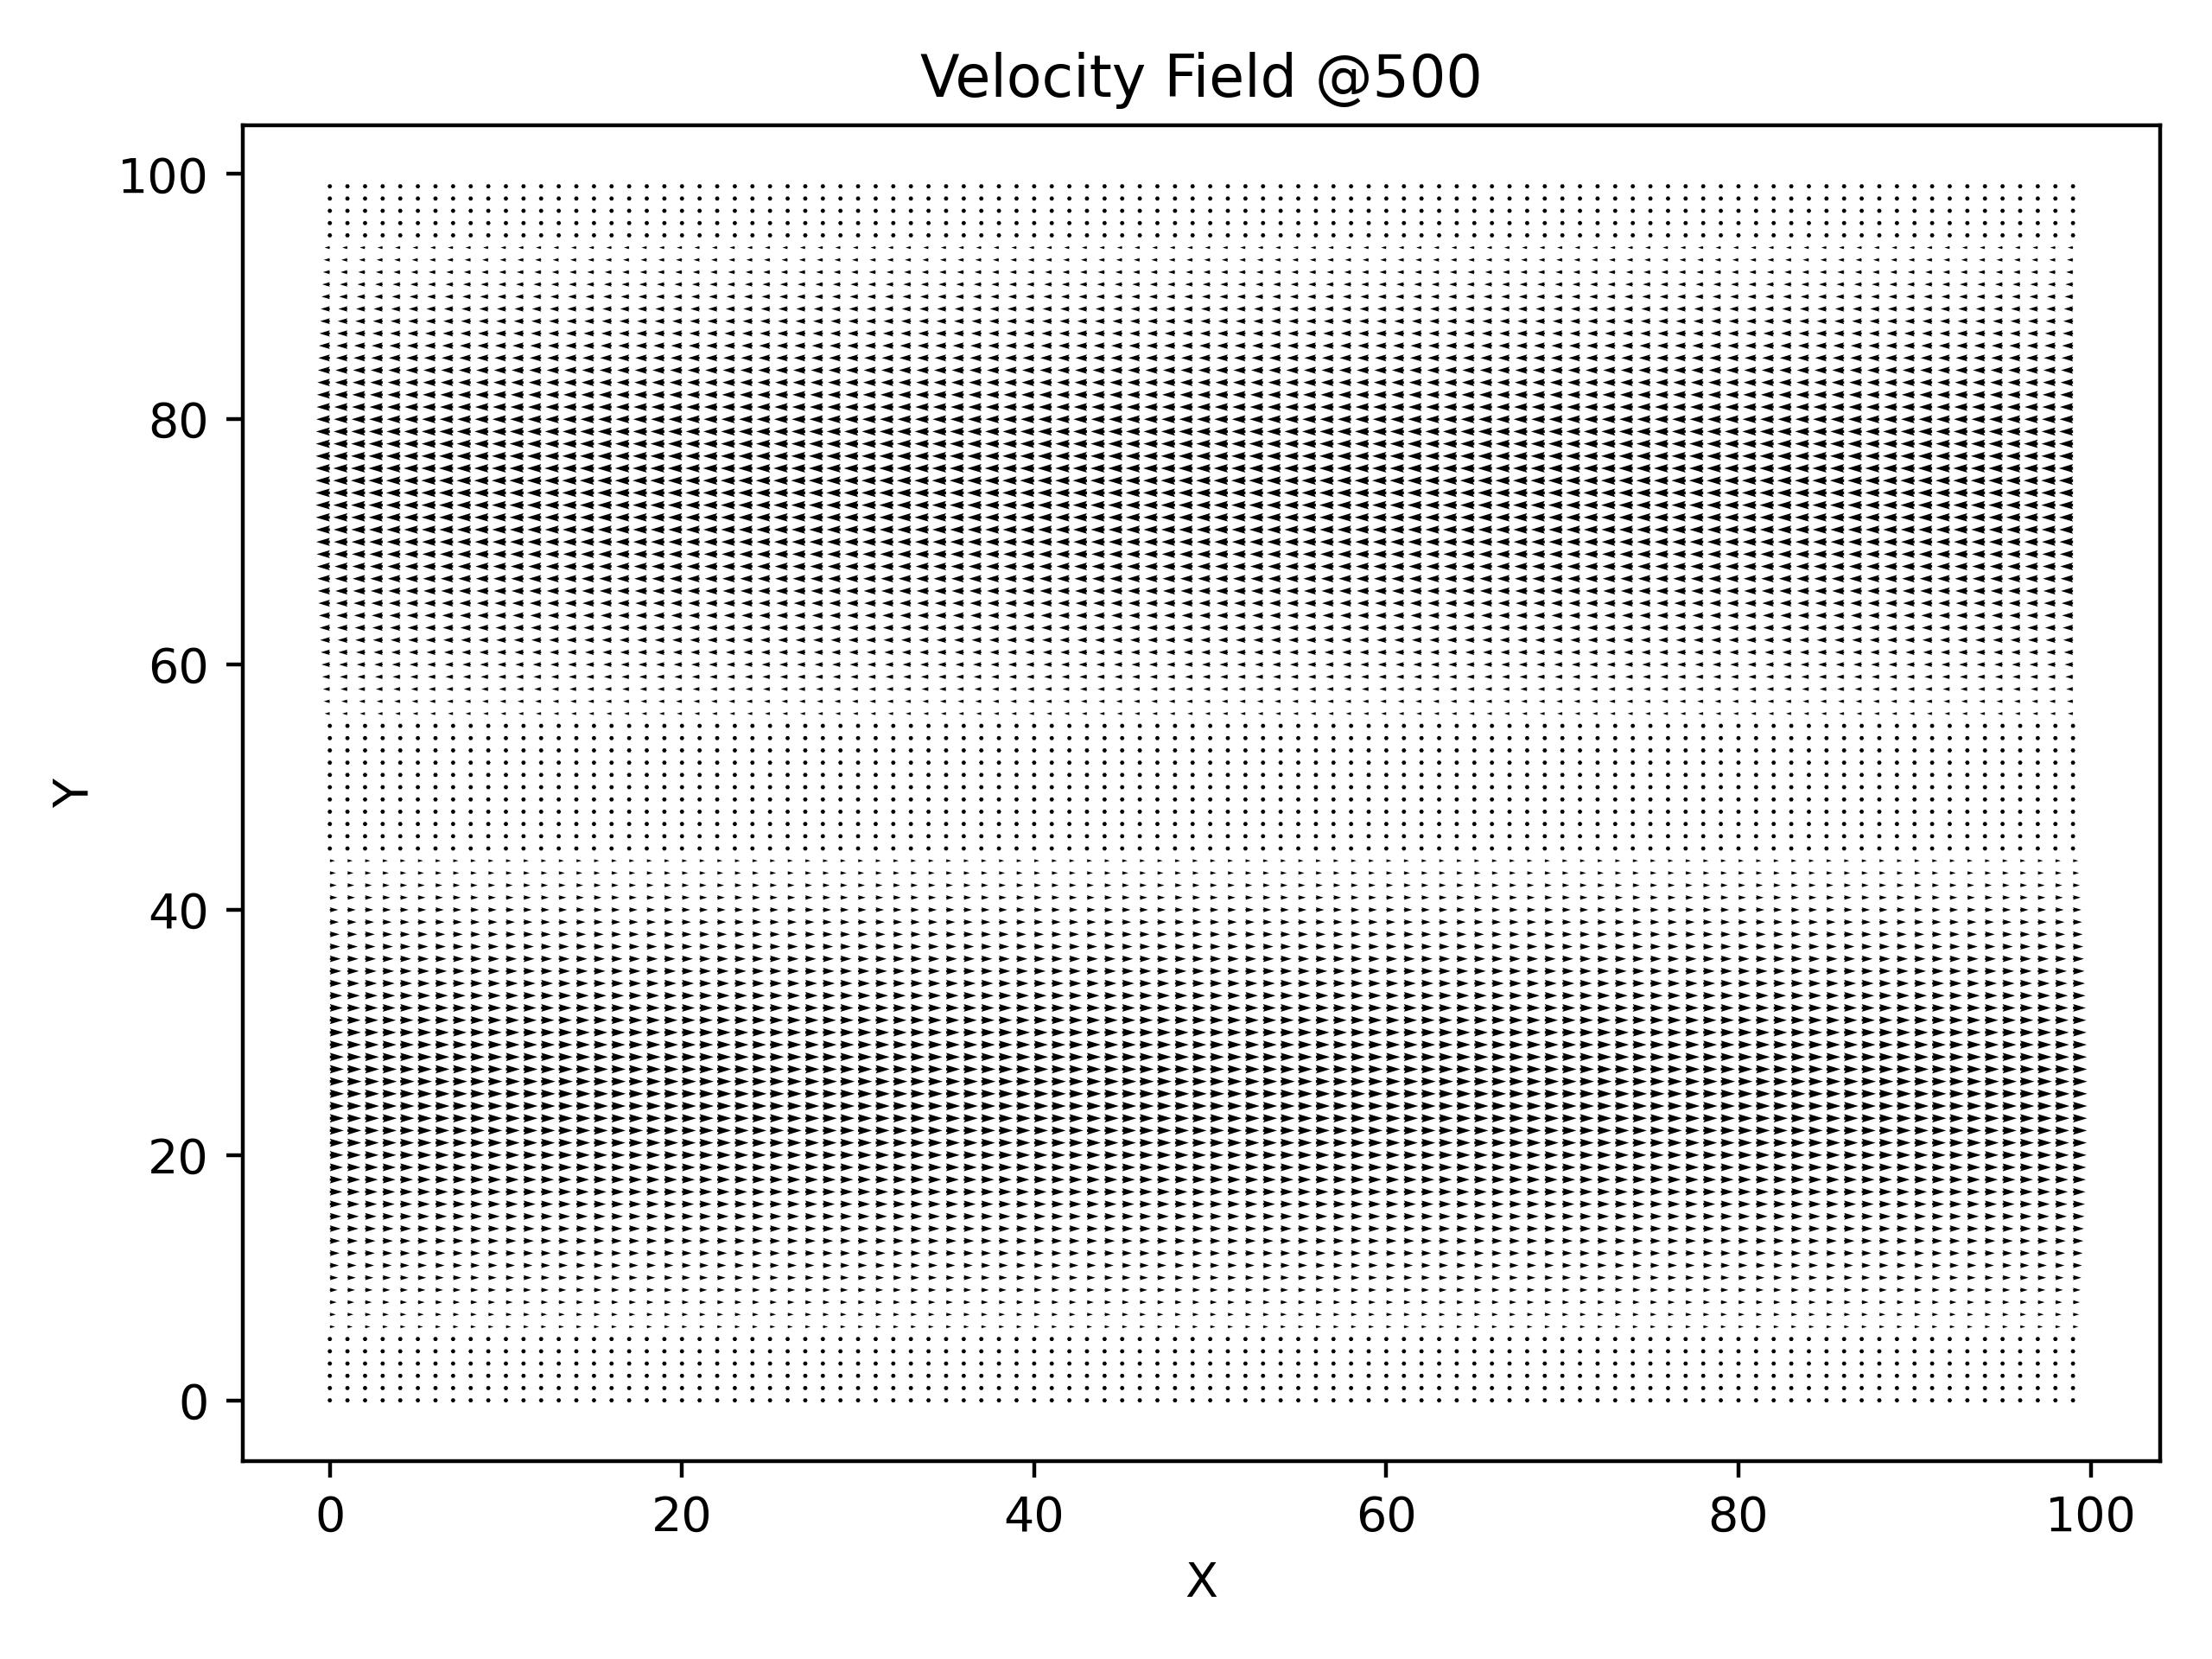
\includegraphics[width=\linewidth]{graphs/ShearWaveDecay/VelocityDistribution/velocity_field_500}
    \end{minipage}% don't remove this comment - uncomments a new line
    \begin{minipage}{0.33\textwidth}
        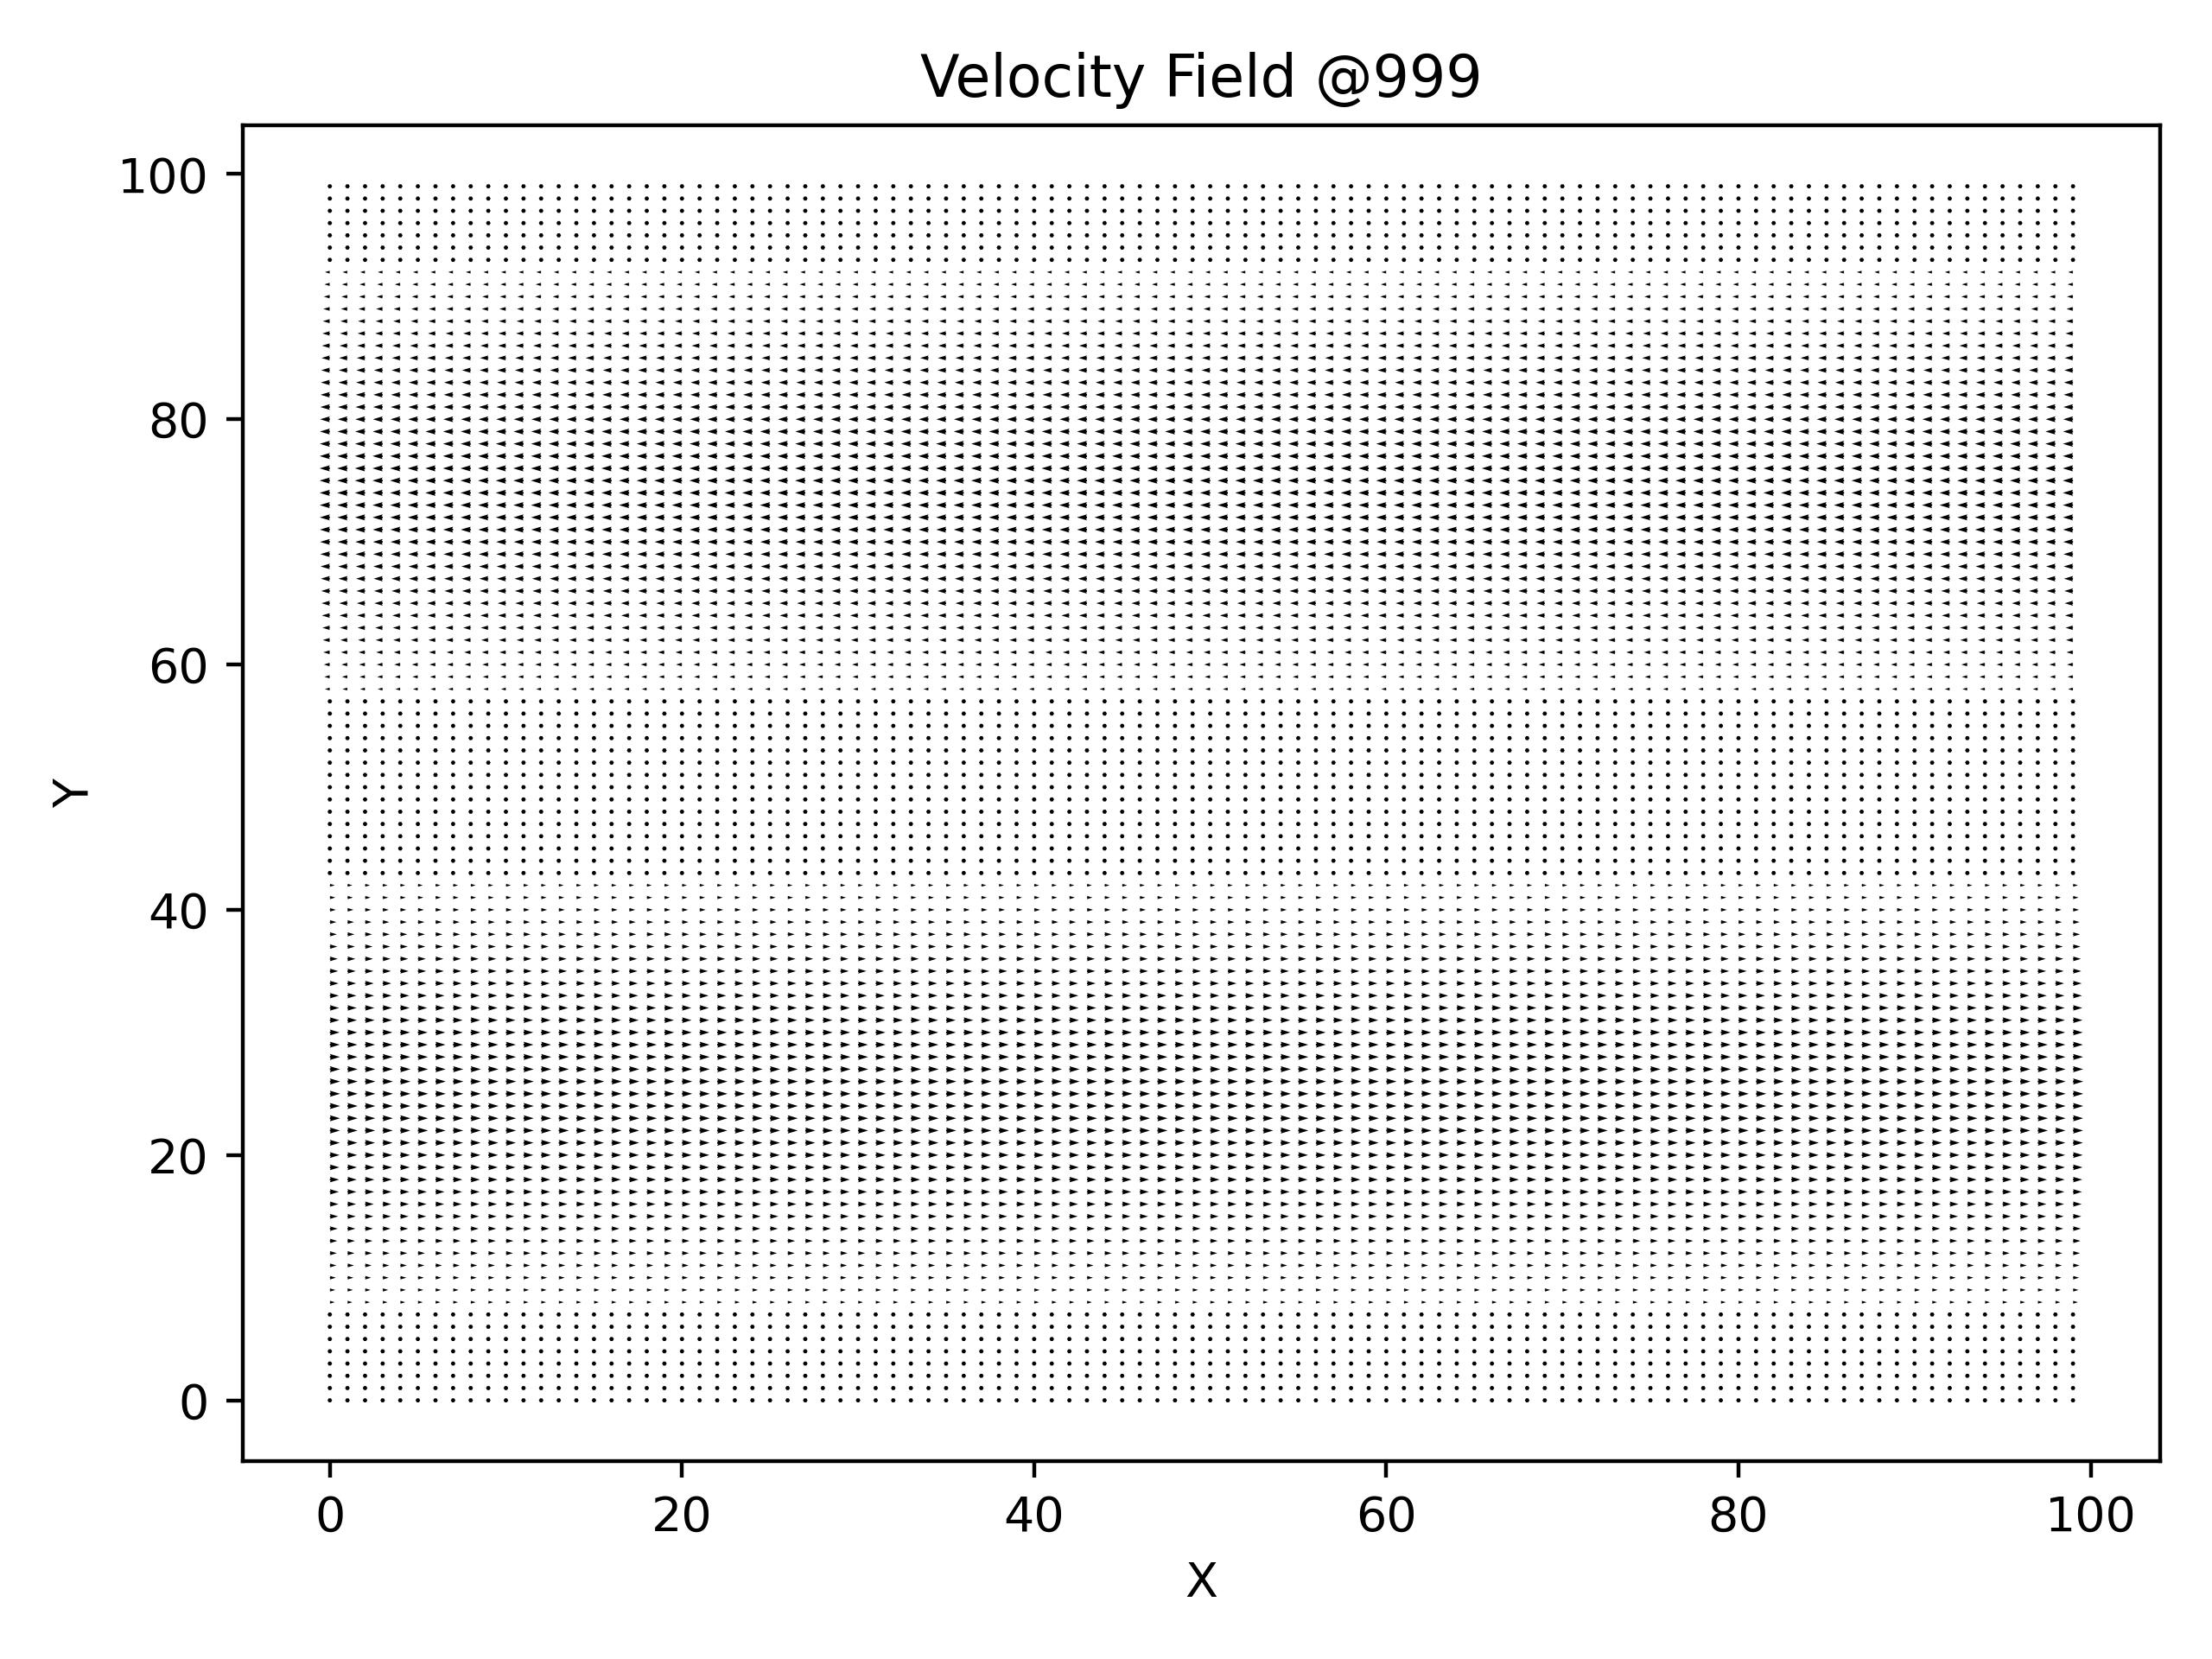
\includegraphics[width=\linewidth]{graphs/ShearWaveDecay/VelocityDistribution/velocity_field_999}
    \end{minipage}
    \caption{
        Different flow states during the simulation.
        From the sinusoid initial condition with a steady decrease till step 999.
    }
    \label{fig:swd-vs-velocity-fields}
\end{figure}

\Cref{fig:swd-vs-velocity-fields} gives a brief overview over the initial flow, and it's decaying over time.
While at step 0, a strong sinusoid flow can be seen, at timestep 999 it decreased visibly.
This decrease can be even further shown in \cref{fig:swd-vs-at-column_x} which shows the decay at a specific column.
The decay rate is also in line with the theoretical solution (as seen in \cref{fig:swd-vs-ideal}) given by
\begin{equation*}
    \begin{aligned}
        a_t &= a_0 e^{-vt \frac{2\pi}{L_y}^2}
    \end{aligned}
\end{equation*}

\begin{center}
    \begin{figure}[h!]
        \begin{minipage}{0.5\textwidth}
            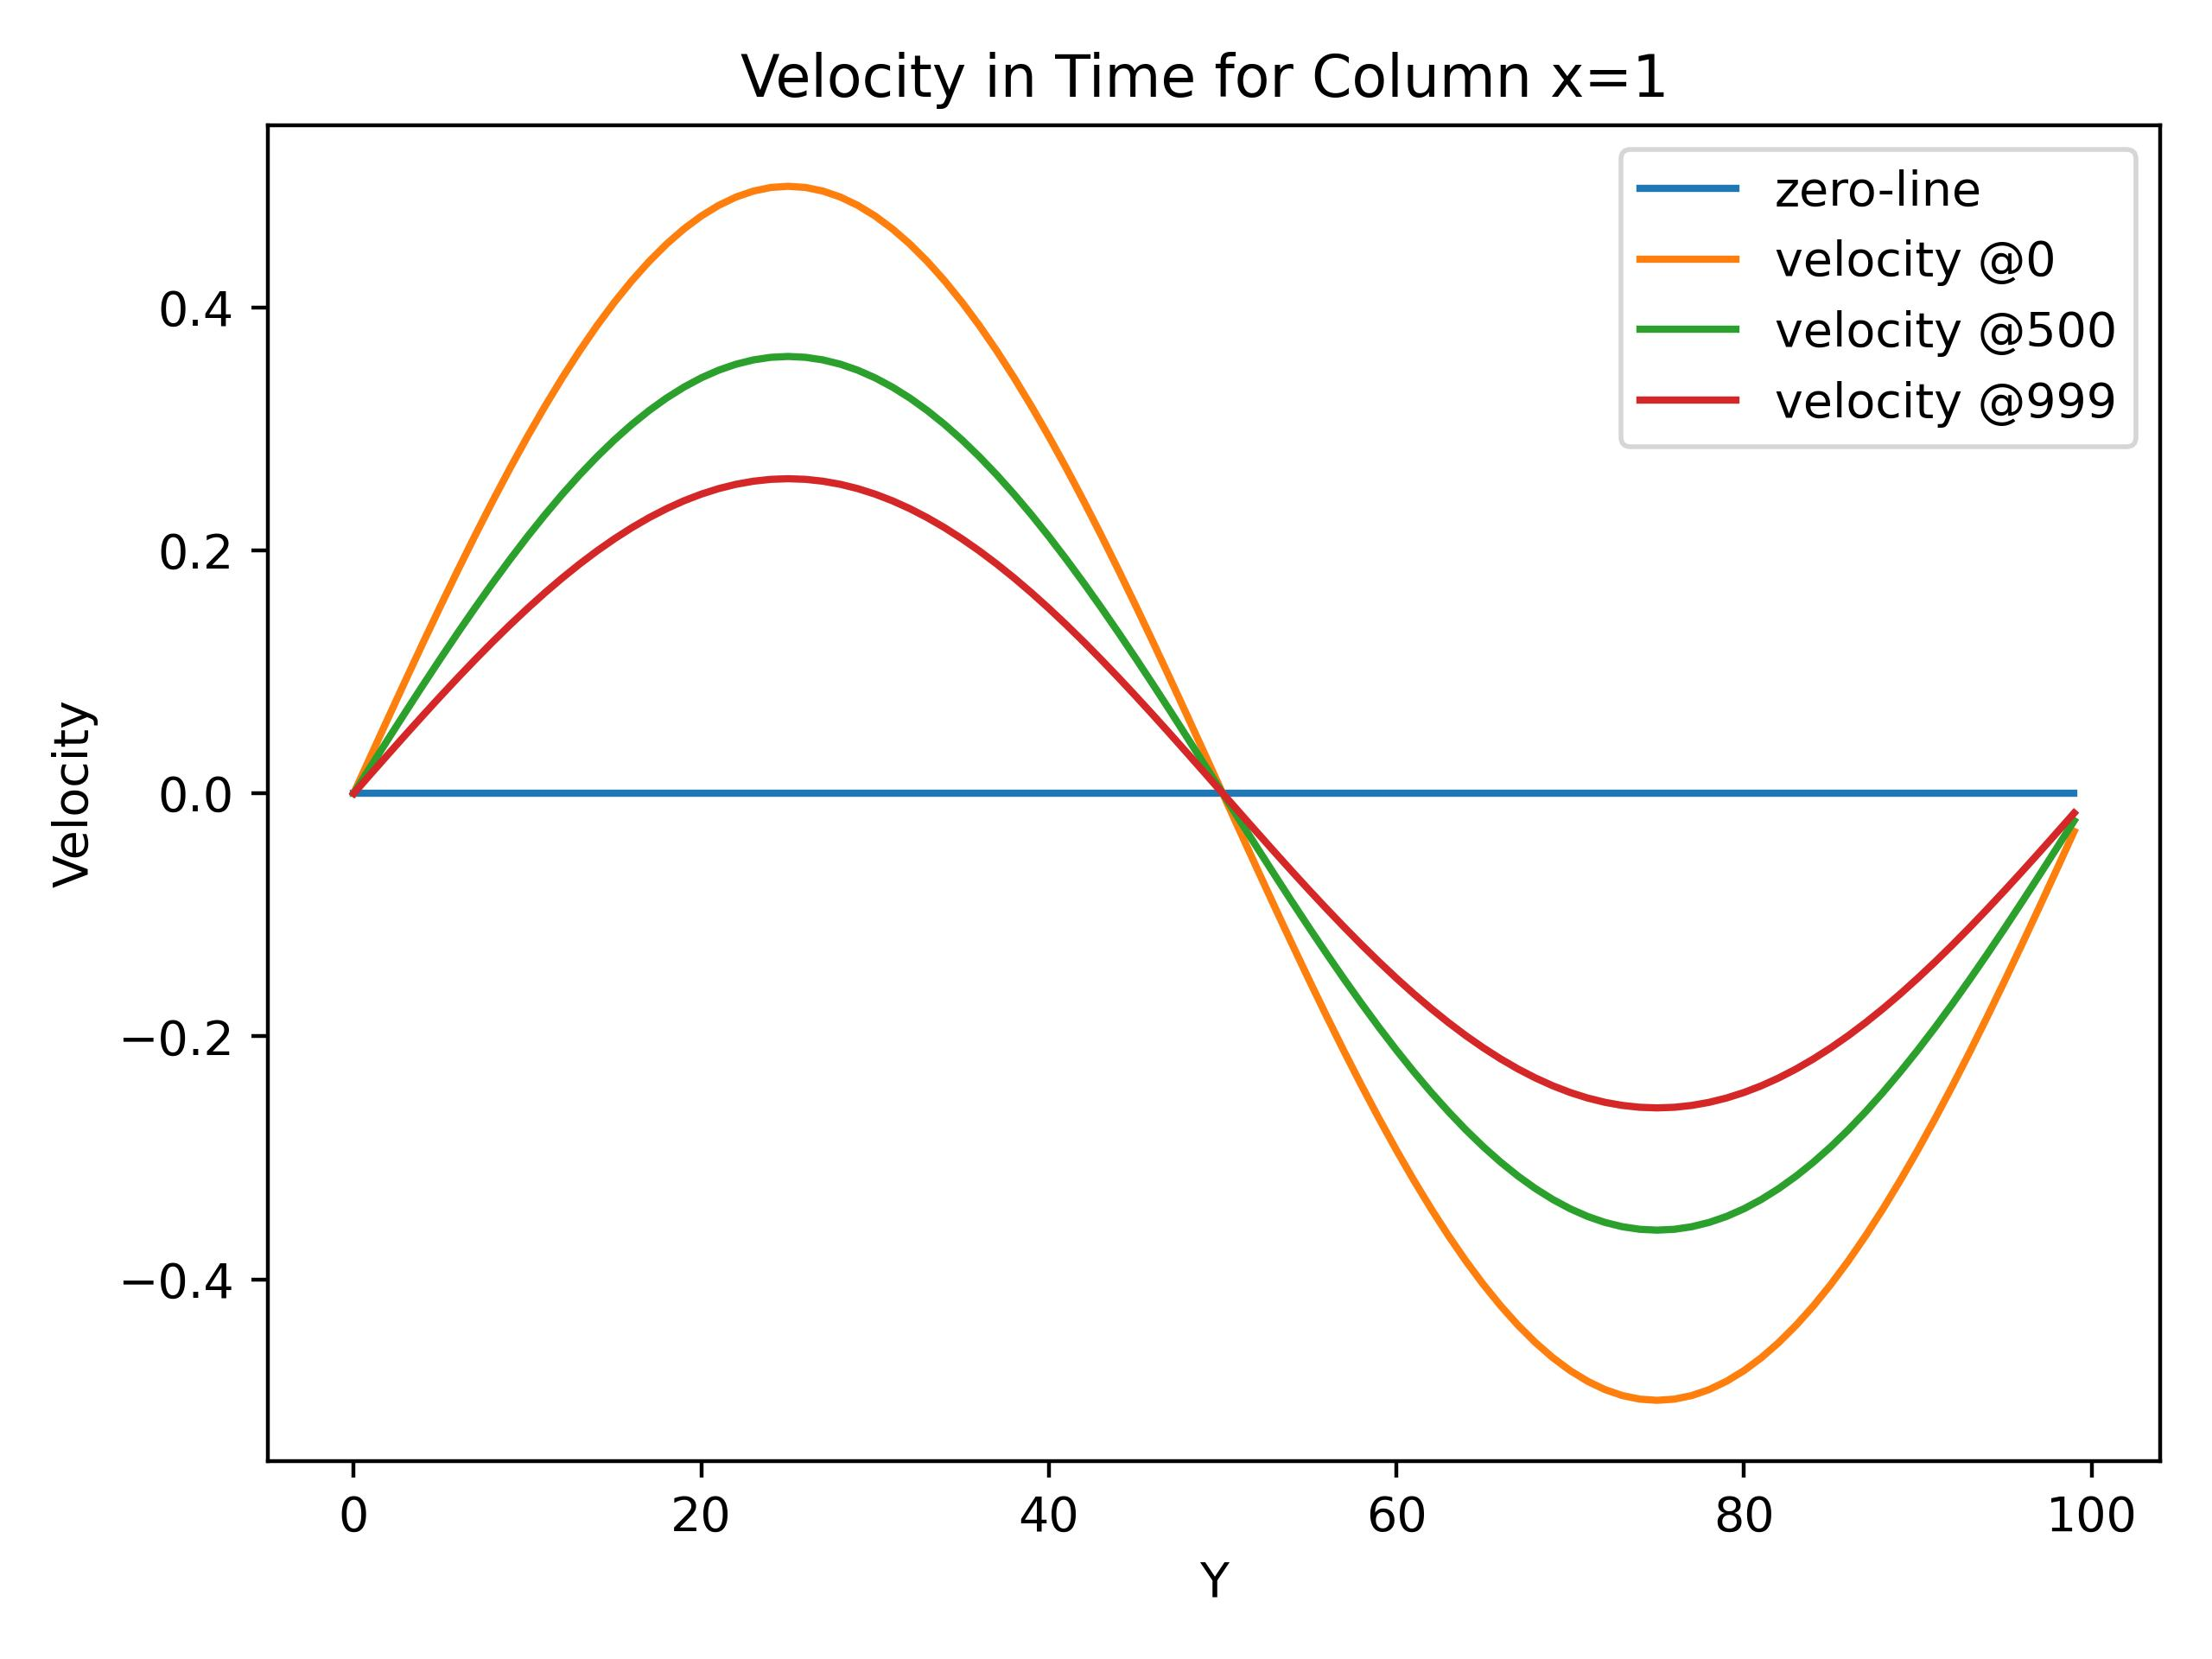
\includegraphics[width=\linewidth]{graphs/ShearWaveDecay/VelocityDistribution/velocity_at_column_x}
            \caption{Decaying velocity at a specific column.}
            \label{fig:swd-vs-at-column_x}
        \end{minipage}% don't remove this comment - uncomments a new line
        \begin{minipage}{0.5\textwidth}
            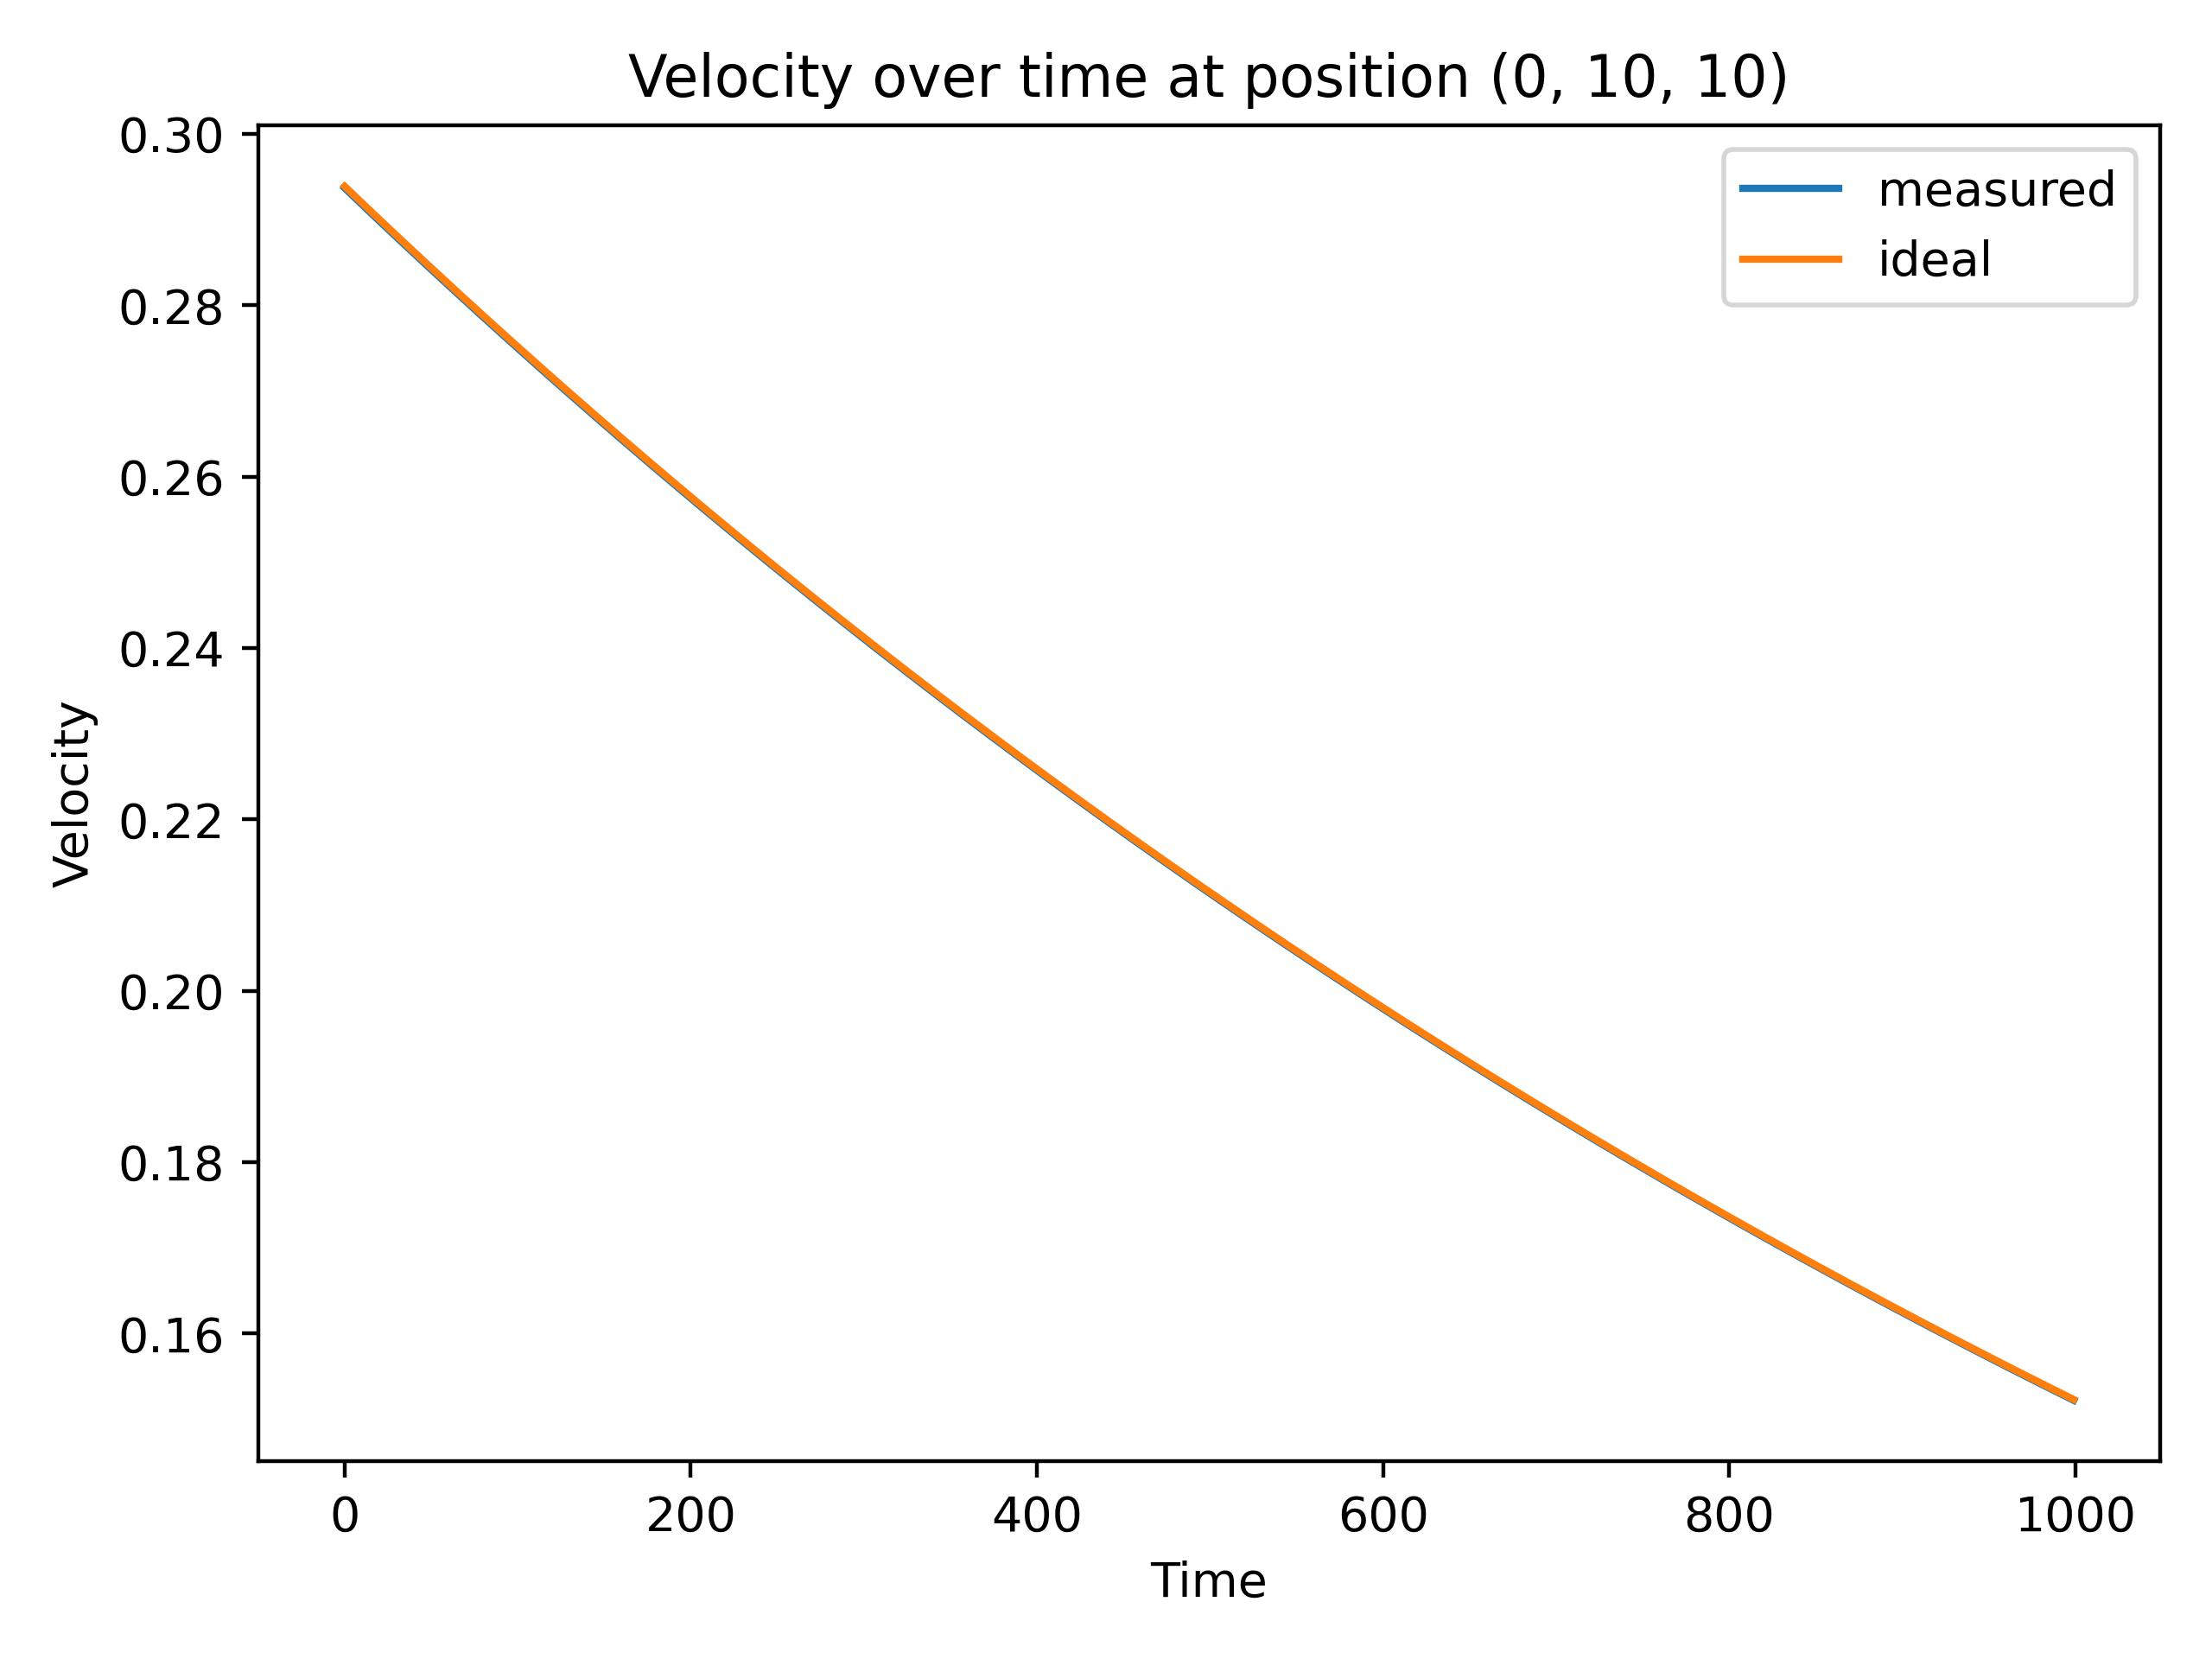
\includegraphics[width=\linewidth]{graphs/ShearWaveDecay/VelocityDistribution/velocity_against_ideal}
            \caption{measured vs ideal decay}
            \label{fig:swd-vs-ideal}
        \end{minipage}
    \end{figure}
\end{center}

\subsection{Correlation of Kinematic Viscosity and Omega}
% TODO in methods: equation to calculate viscosity from experiment
This experiment aims to measure the correlation between the kinematic viscosity and the parameter omega, that is used for the collision.
The kinematic viscosity describes, how \textit{thick} some fluid is, e.g.\ syrup has a higher viscosity than water. % https://en.wikipedia.org/wiki/Viscosity
This experiment measures the viscosity by running the previous experiment \cref{subsec:sinusoidal-velocity} multiple times with different omegas.
It is expected that a lower omega has a higher viscosity. % TODO why?
The results of the experiment are shown in \cref{fig:swd-vo-viscosity-vs-omega}.

\begin{figure}[h!]
    \begin{center}
        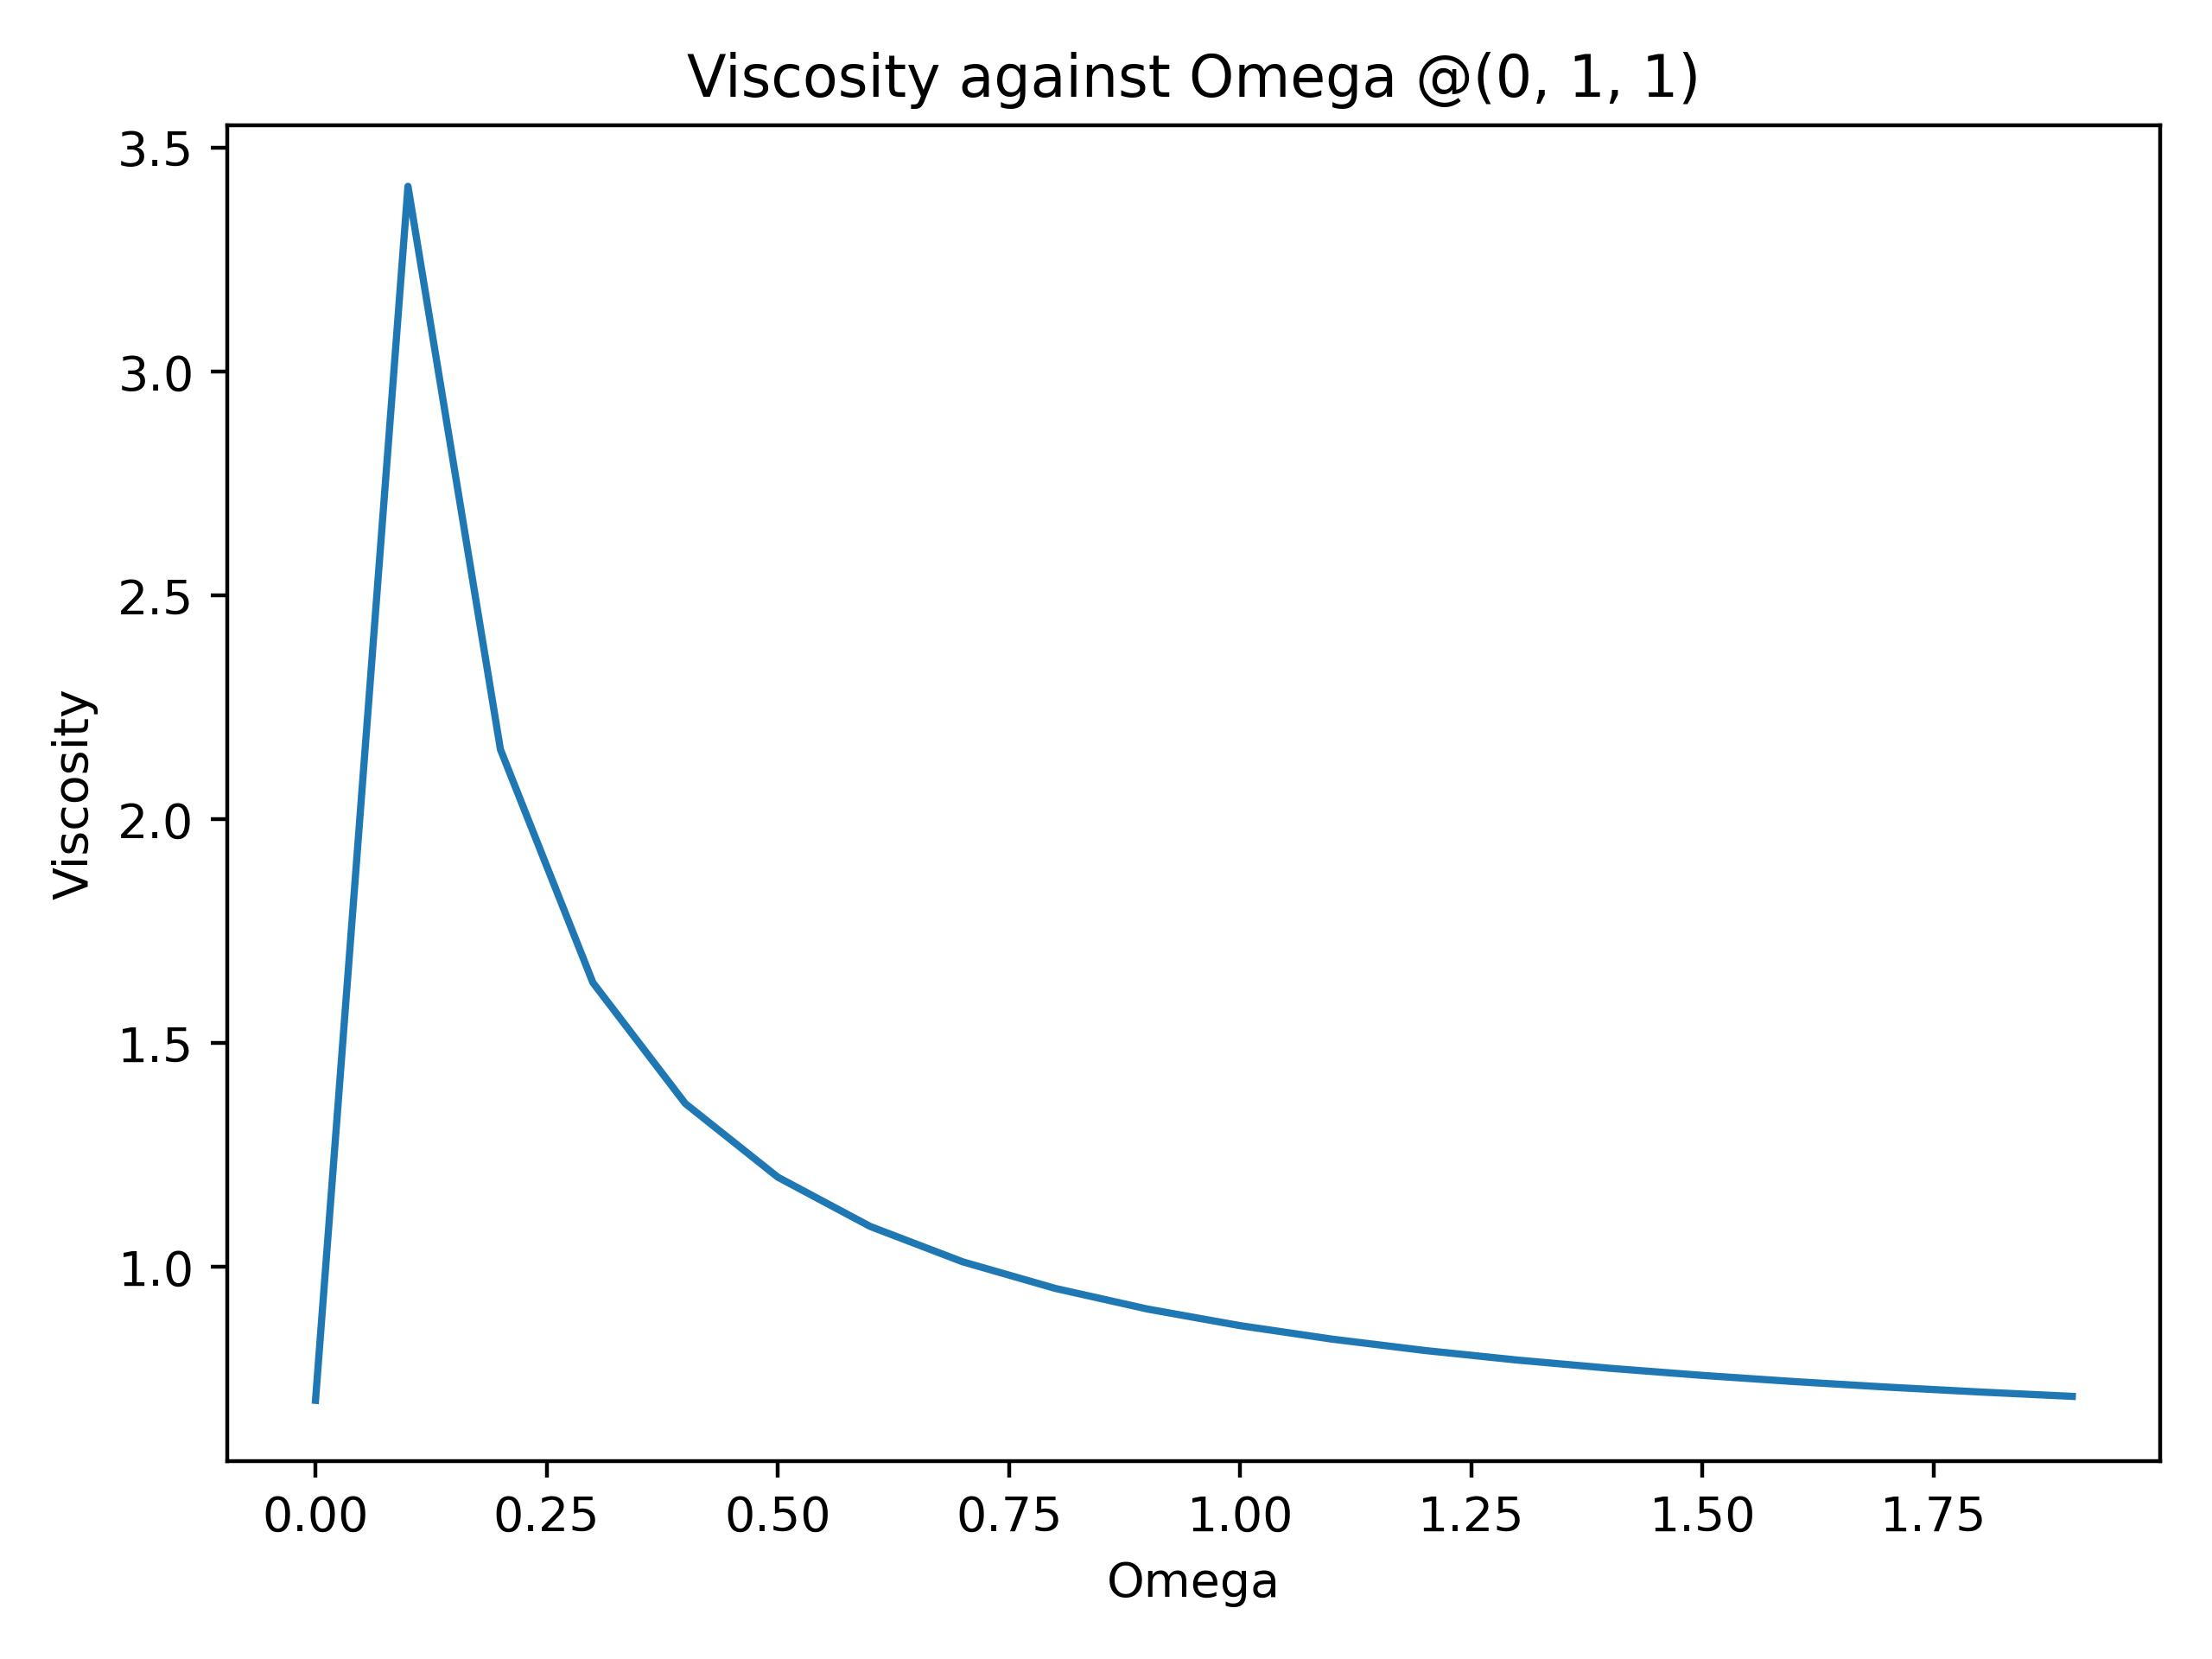
\includegraphics[width=0.5\linewidth]{graphs/ShearWaveDecay/Viscosity/viscosity_against_omega}
        \caption{Correlation between the kinematic viscosity and omega.}
        \label{fig:swd-vo-viscosity-vs-omega}
    \end{center}
\end{figure}

Strangely, for very small omega, the viscosity does not follow the otherwise exponential decay.
This is due to the model of the simulation, that fails to replicate the exact behaviour with too large or small values. % TODO why?
In theory, this may even have an impact on the experiments, but omega was set to 1.0 to not have a negative impact of this phenomenon.


\section{Couette Flow}
The \textit{Couette Flow} arises in a bounded field with two distinct boundaries located at the top and bottom.
Notably, the lower boundary remains stationary, while the upper boundary is sliding in x-direction.
Periodic boundary conditions are enforced along the right and left sides.
The initial condition, depicted in \cref{fig:cf-initial-condition} and can be mathematically expressed as follows:
\begin{equation*}
    \begin{aligned}
        \rho(0) = 0 \\
        \mathbf{u}(0) = 0 \cdot
    \end{aligned}
\end{equation*}

\begin{figure}[h!]
    \begin{center}
        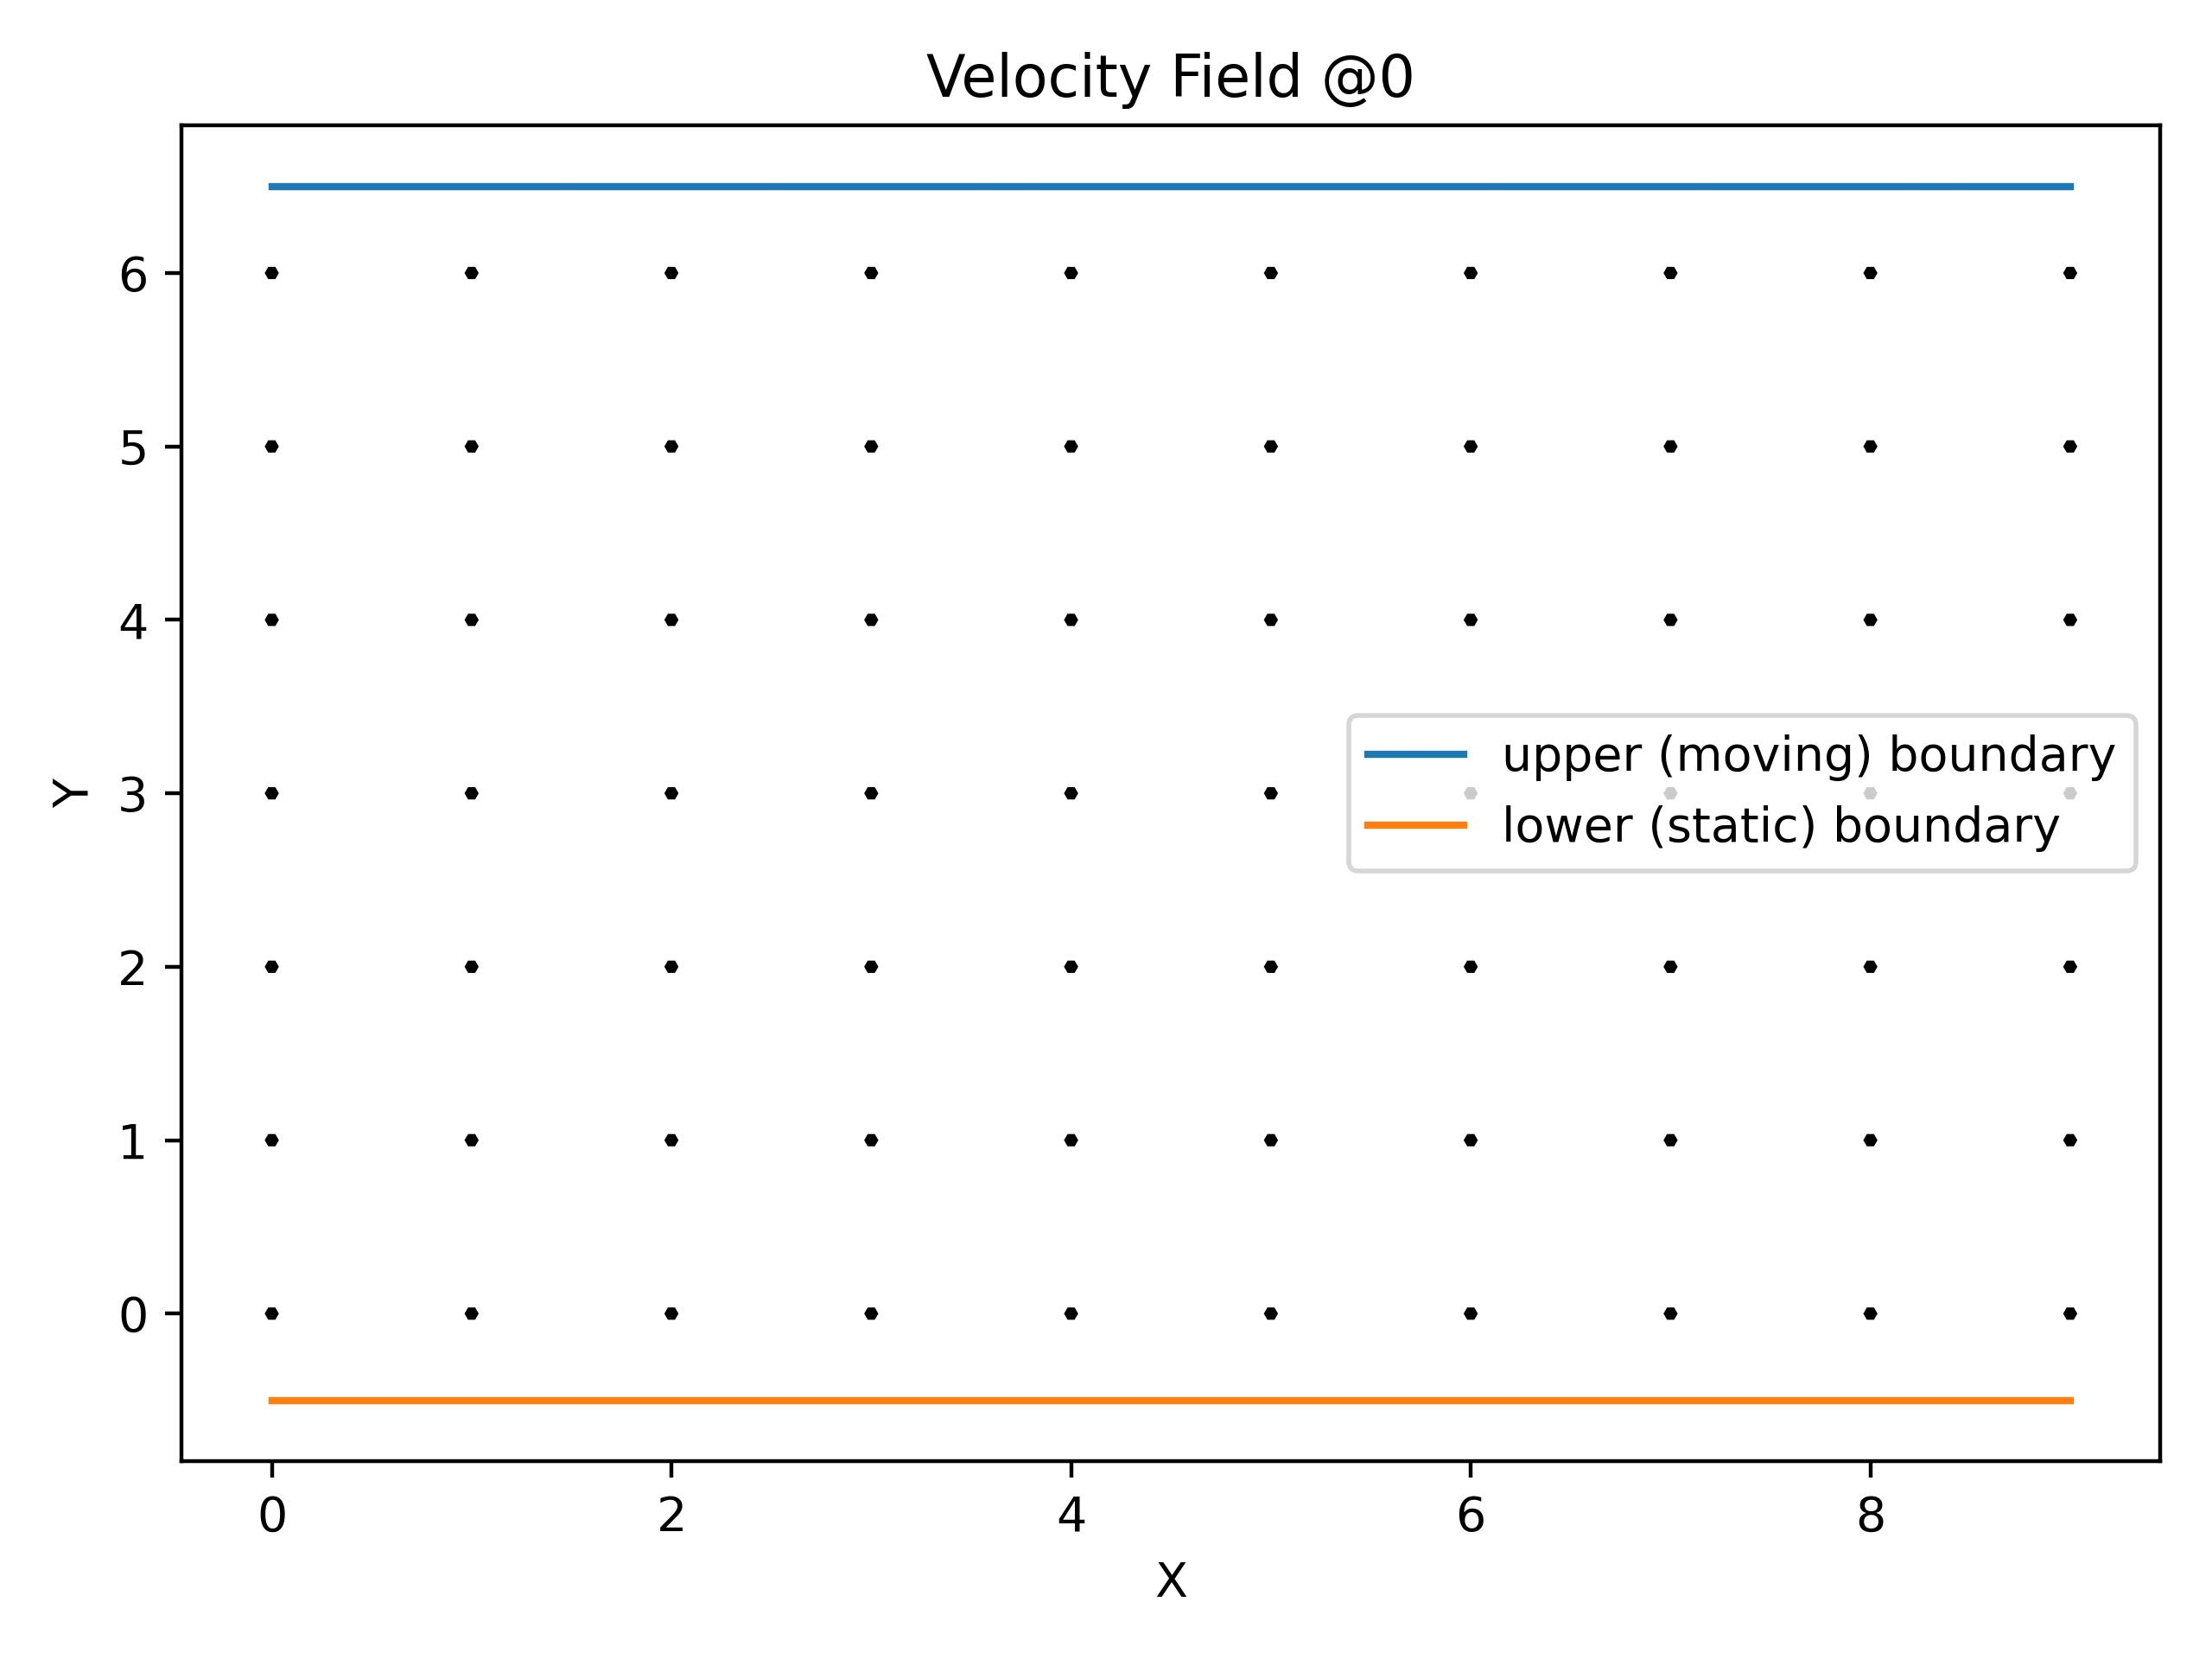
\includegraphics[width=0.5\linewidth]{graphs/CouetteFlow/velocity_field_couette_flow_0}
        \caption{Initial condition with a sliding boundary at the top, periodic boundary conditions to the side and a hard wall to the bottom.}
        \label{fig:cf-initial-condition}
    \end{center}
\end{figure}

Because of the friction of the boundaries, the fluid starts flow.
More specifically, the fluid in the top starts to get momentum, because it is close to the upper boundary which is moving.
This flow then spreads further down.
But because the wall at the bottom is steady, the flow gets less the further it deepens.
This process can be seen in the following two graphs in \cref{fig:cf-velocity-field-over-time}.


\begin{center}
    \begin{figure}[h!]
        \begin{minipage}{0.5\textwidth}
            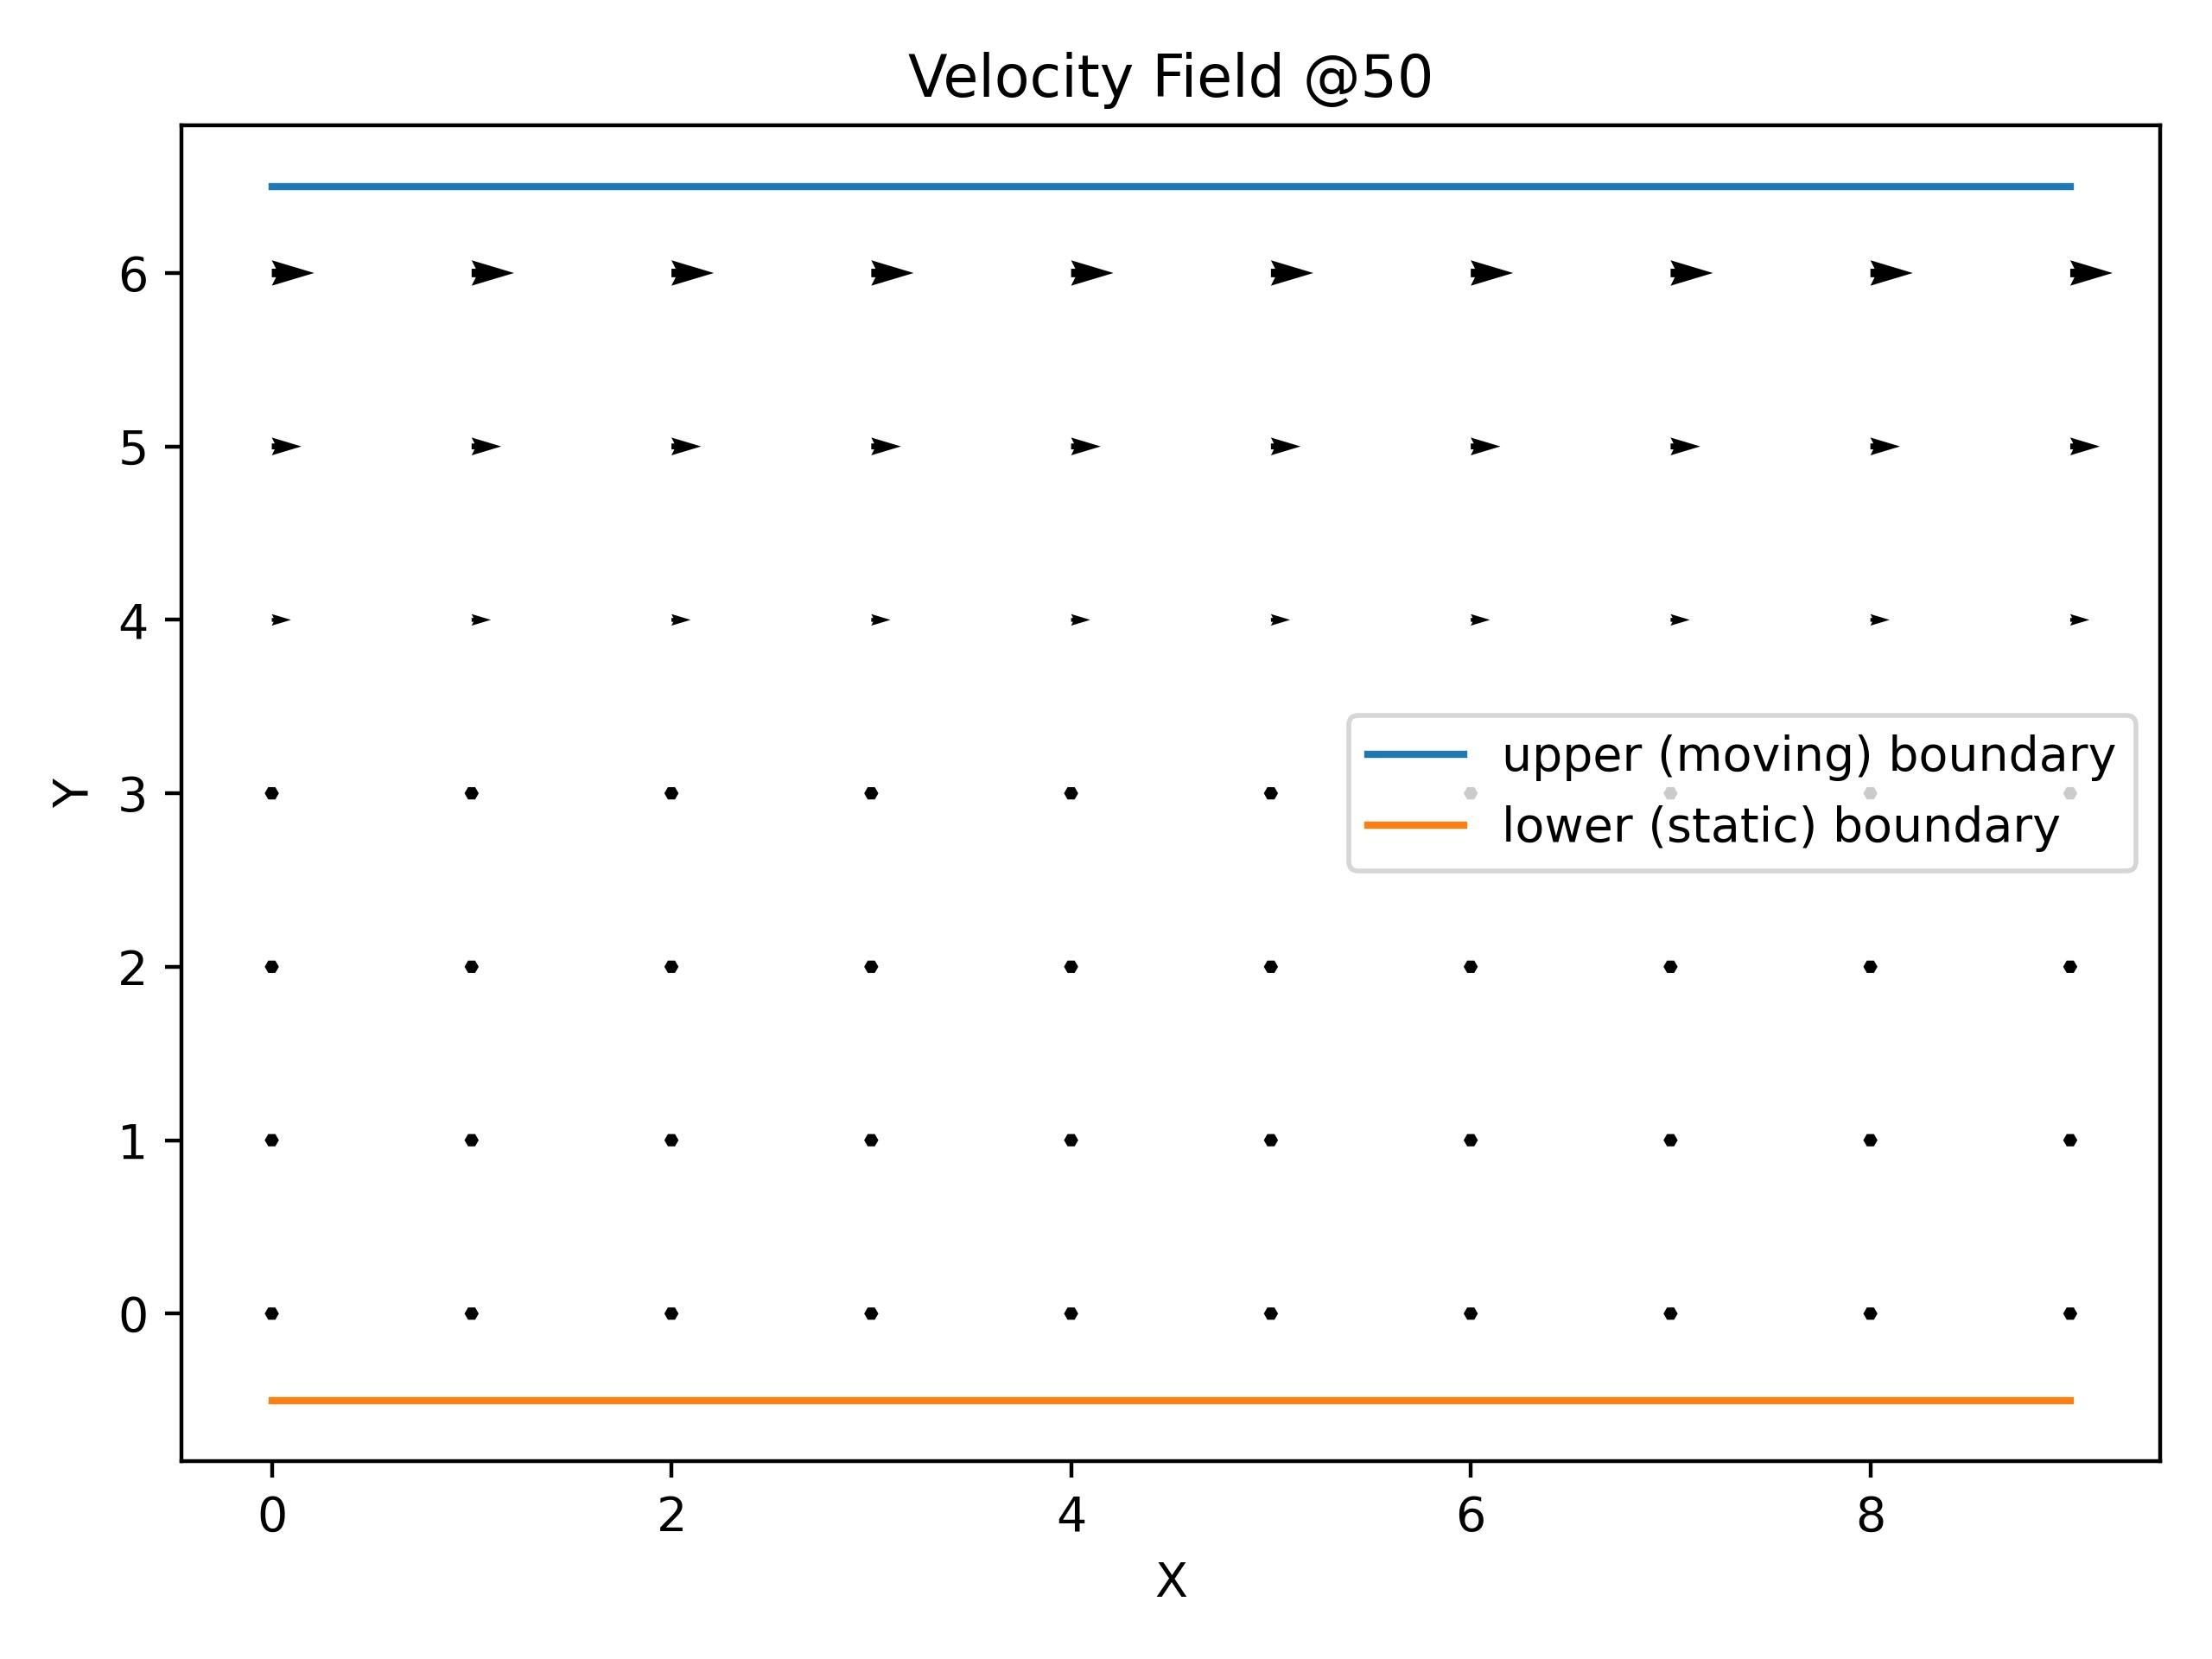
\includegraphics[width=\linewidth]{graphs/CouetteFlow/velocity_field_couette_flow_50}
        \end{minipage}% don't remove this comment - uncomments a new line
        \begin{minipage}{0.5\textwidth}
            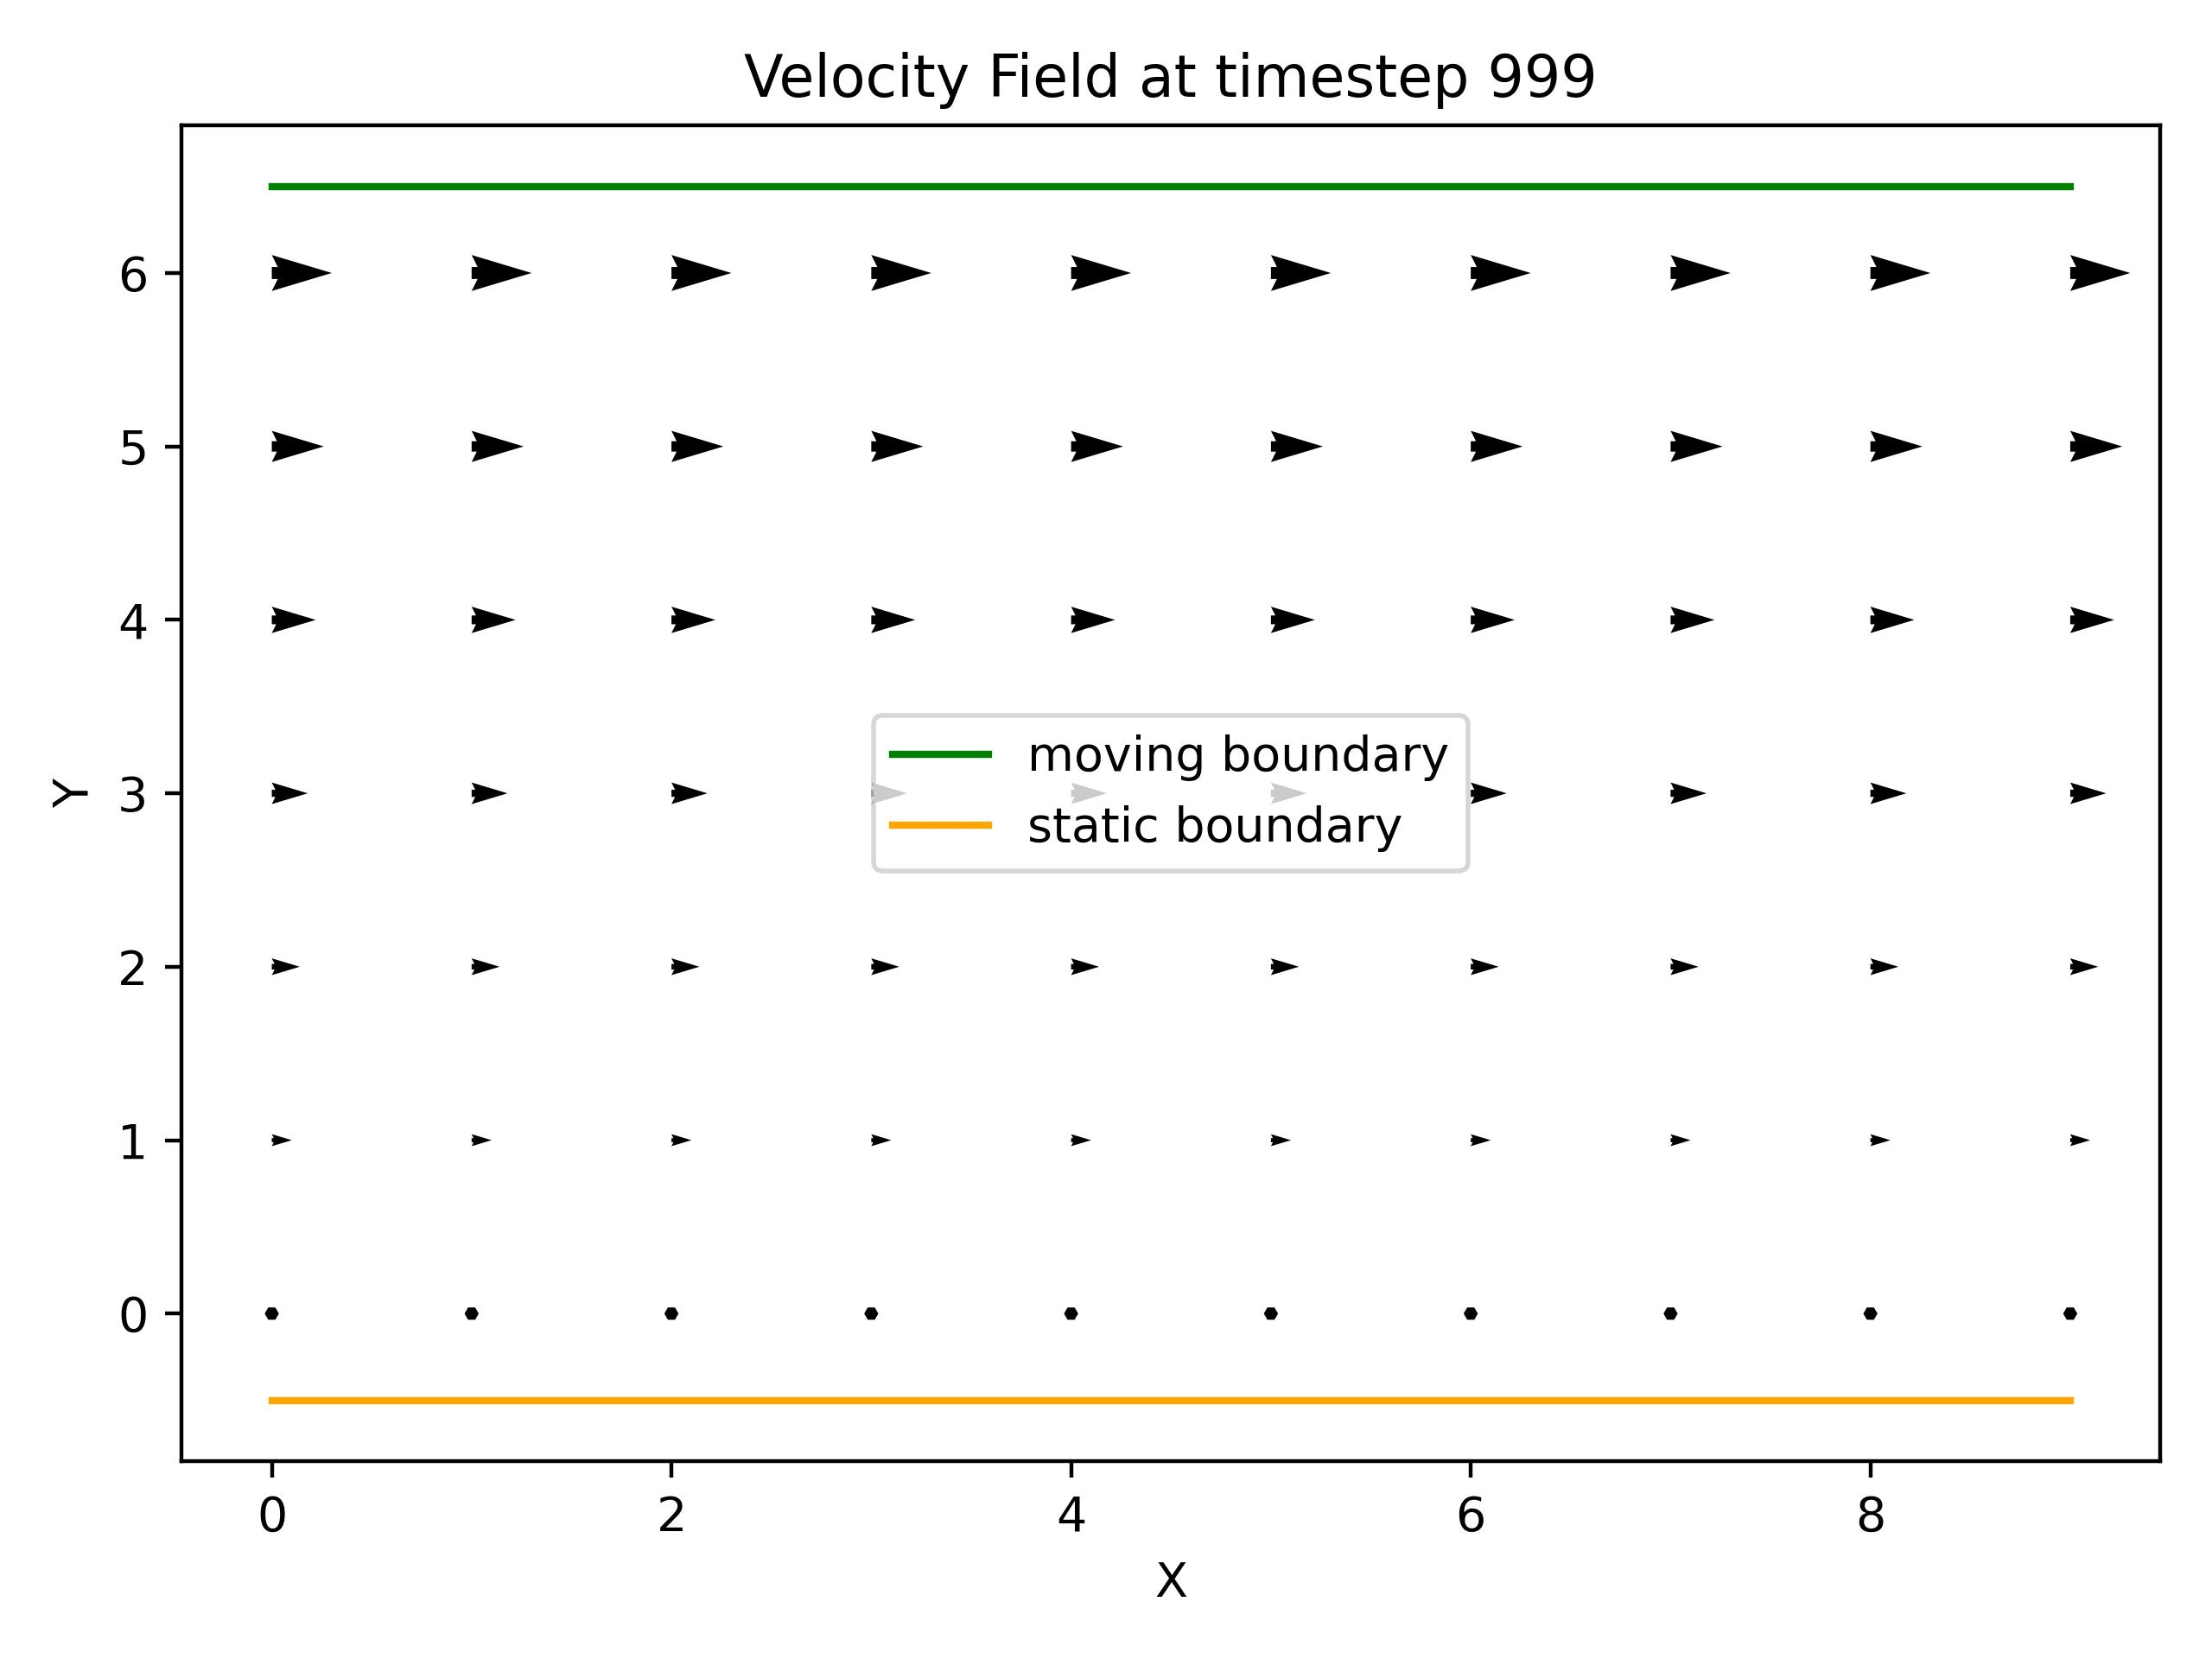
\includegraphics[width=\linewidth]{graphs/CouetteFlow/velocity_field_couette_flow_999}
        \end{minipage}
        \caption{Velocity field of Couette Flow over time.}
        \label{fig:cf-velocity-field-over-time}
    \end{figure}
\end{center}

To reproduce this experiment, please use the parameters from \cref{tab:cf-parameters}.

\begin{table}[ht]
    \centering % used for centering table
    \begin{tabular}{c c}
% centered columns (4 columns)
        \hline\hline %inserts double horizontal lines
        Parameter   & Value \\ [0.5ex] % inserts table heading
        \hline % inserts single horizontal line
        $L_x$       & 10    \\
        $L_y$       & 10    \\
        $\omega$    & 1.0   \\
        $\epsilon$  & 0.01  \\
        sliding u   & -0.1  \\
        sliding rho & 1     \\
        $t_{\max}$  & 1000  \\ [1ex] % [1ex] adds vertical space
        \hline %inserts single line
    \end{tabular}
    \caption{Parameters for the Couette Flow} % title of Table
    \label{tab:cf-parameters}
\end{table}


\section{Poiseuille Flow}
The \textit{Poiseuille Flow} can be described as a pressure pipe.
There are stationary boundaries at the top and bottom and a periodic boundary condition to the sides.
In the beginning all velocity is set to 0 as defined by the initial condition
\begin{equation*}
    \begin{aligned}
        \rho(0) &= 1.0 \\
        \mathbf{u}(0) &= 0 \cdot
    \end{aligned}
\end{equation*}

Because of the pressure, a flow starts from one side to the other and maxes out at a certain speed given by the pressure.
The resulting velocity field is shown in \cref{fig:pf-velocity-field}.
\begin{figure}[h!]
    \begin{center}
        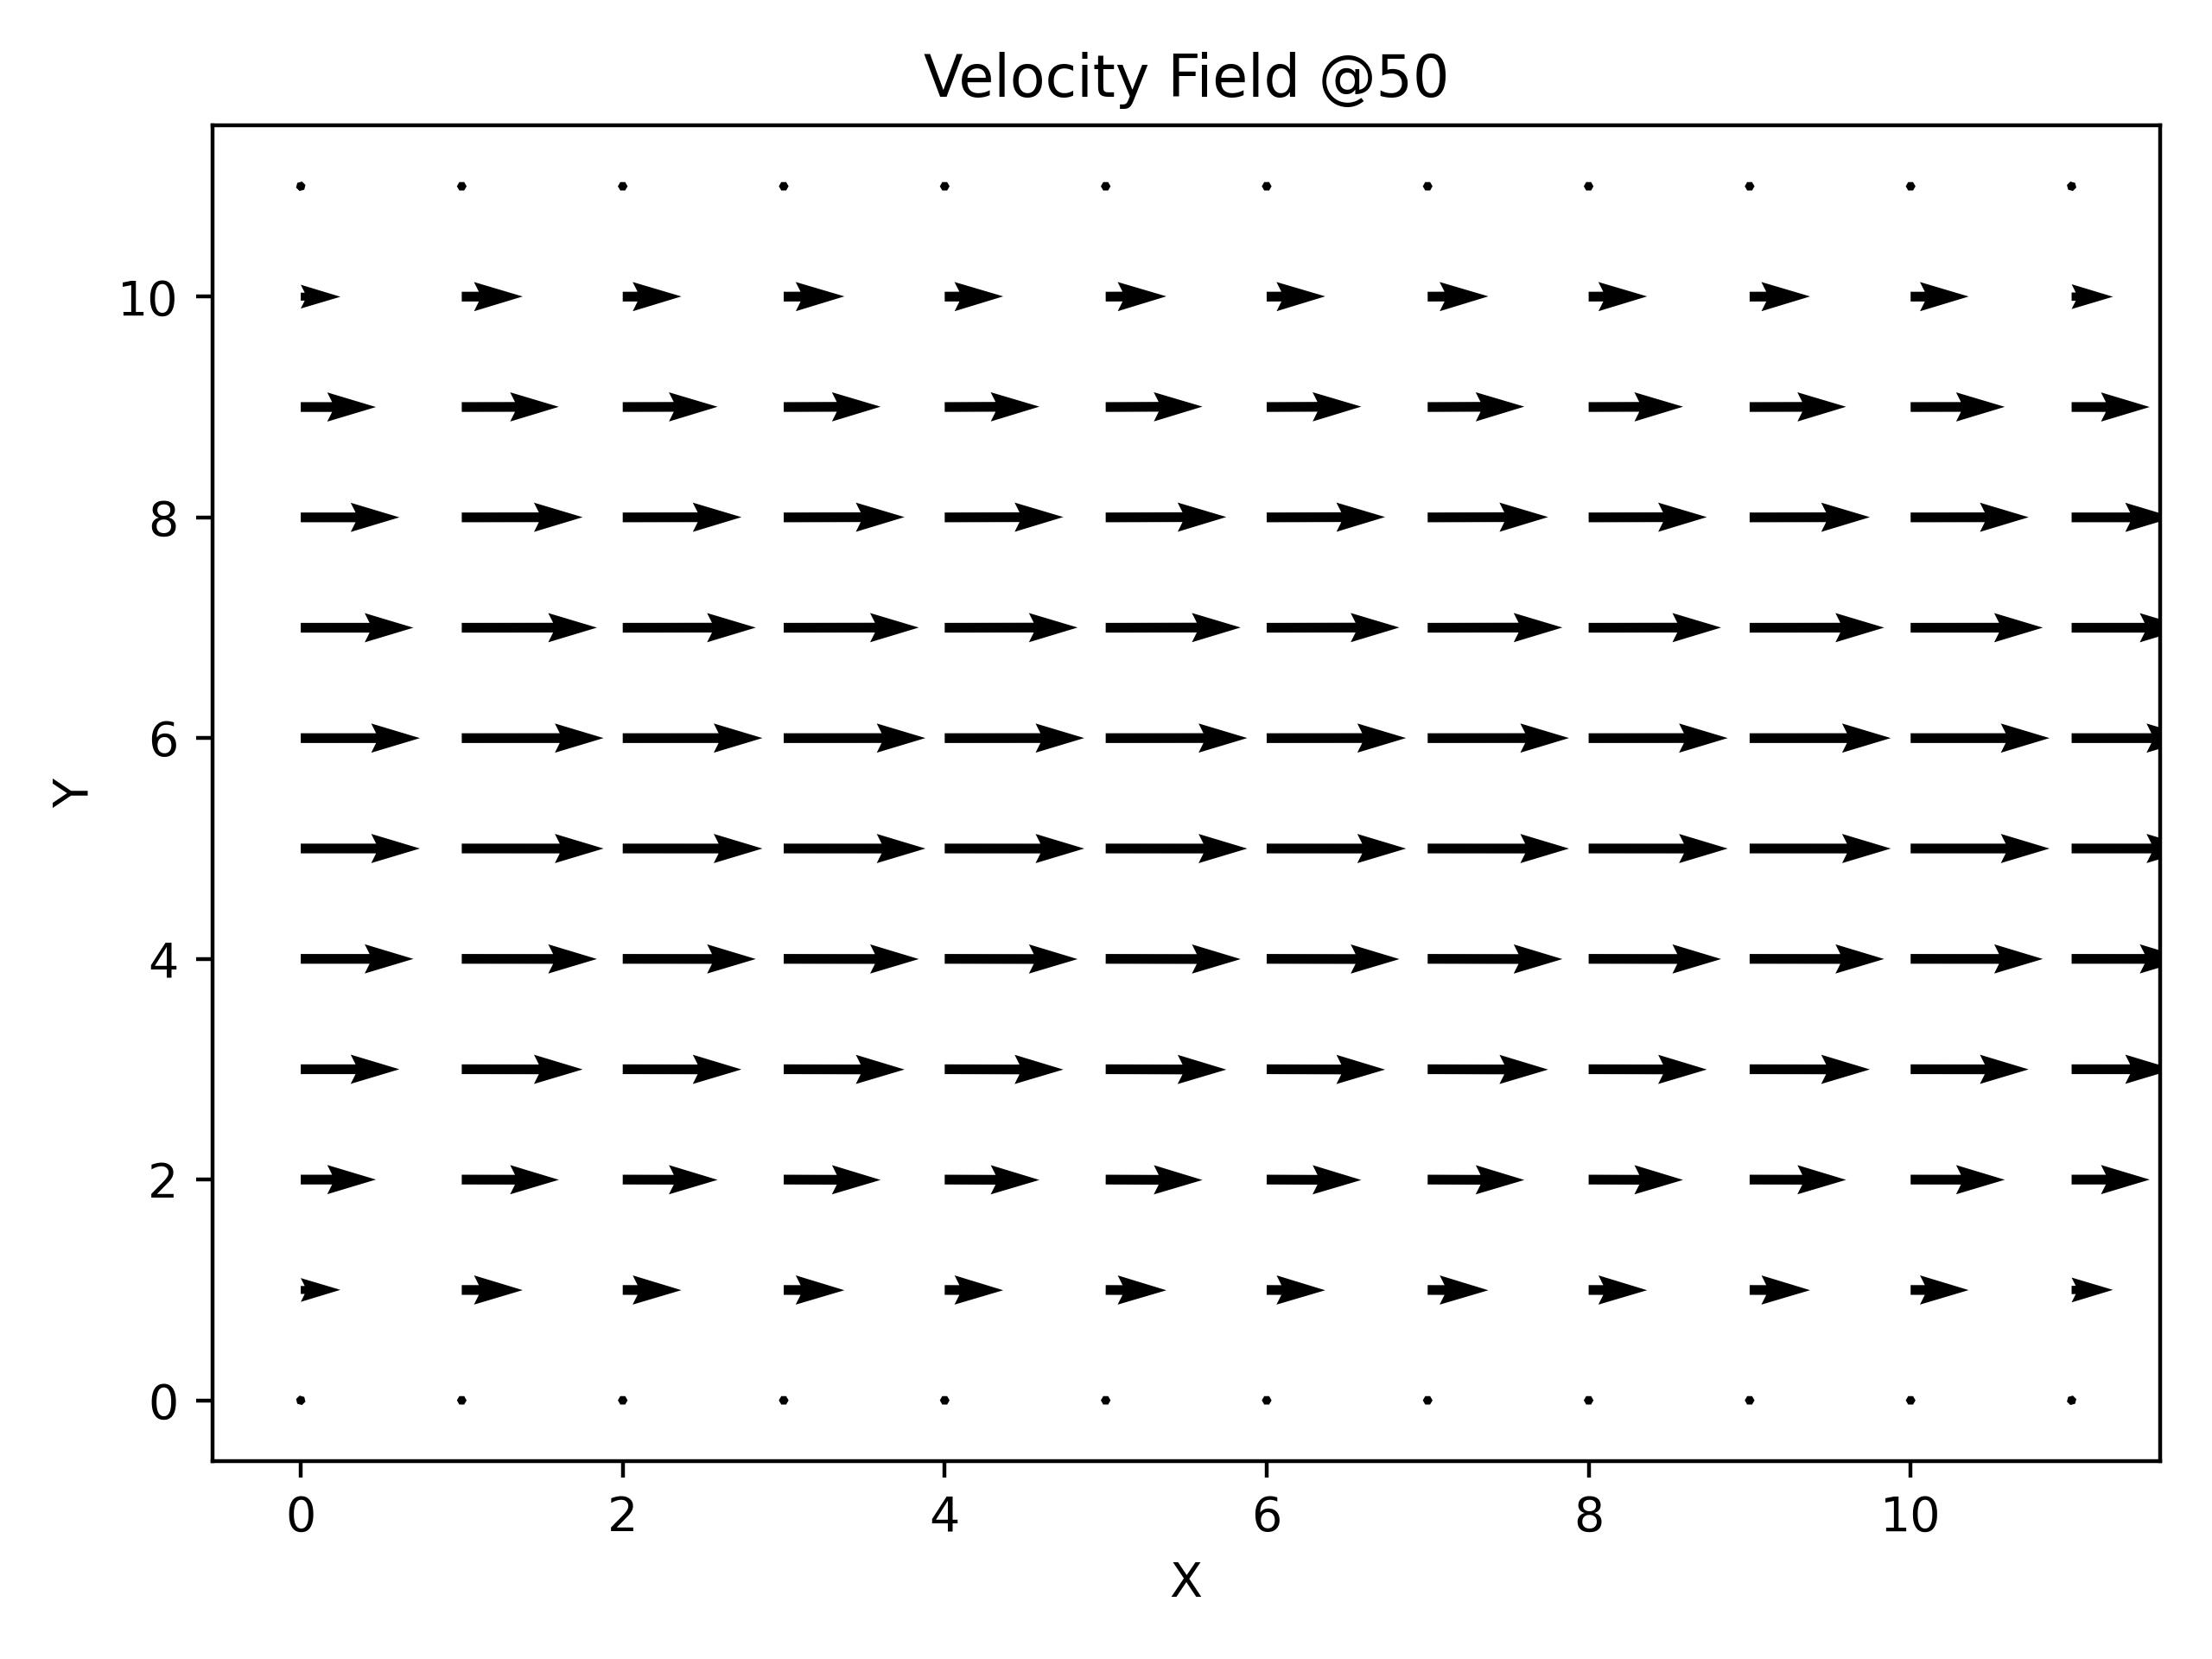
\includegraphics[width=0.5\linewidth]{graphs/PoiseuilleFlow/velocity_field_50}
        \caption{The steady state of the Poiseuille Flow.}
        \label{fig:pf-velocity-field}
    \end{center}
\end{figure}

The velocity field inside the pipe changes as shown in \cref{fig:pf-velocity-areas}.
It can be clearly seen, that the amount of viscosity is first higher at the start of the pipe, near the pressure difference.
While the experiment continuous, the velocity adjusts throughout further in the pipe until it is the same.


\begin{figure}[h!]
    \begin{minipage}{0.33\textwidth}
        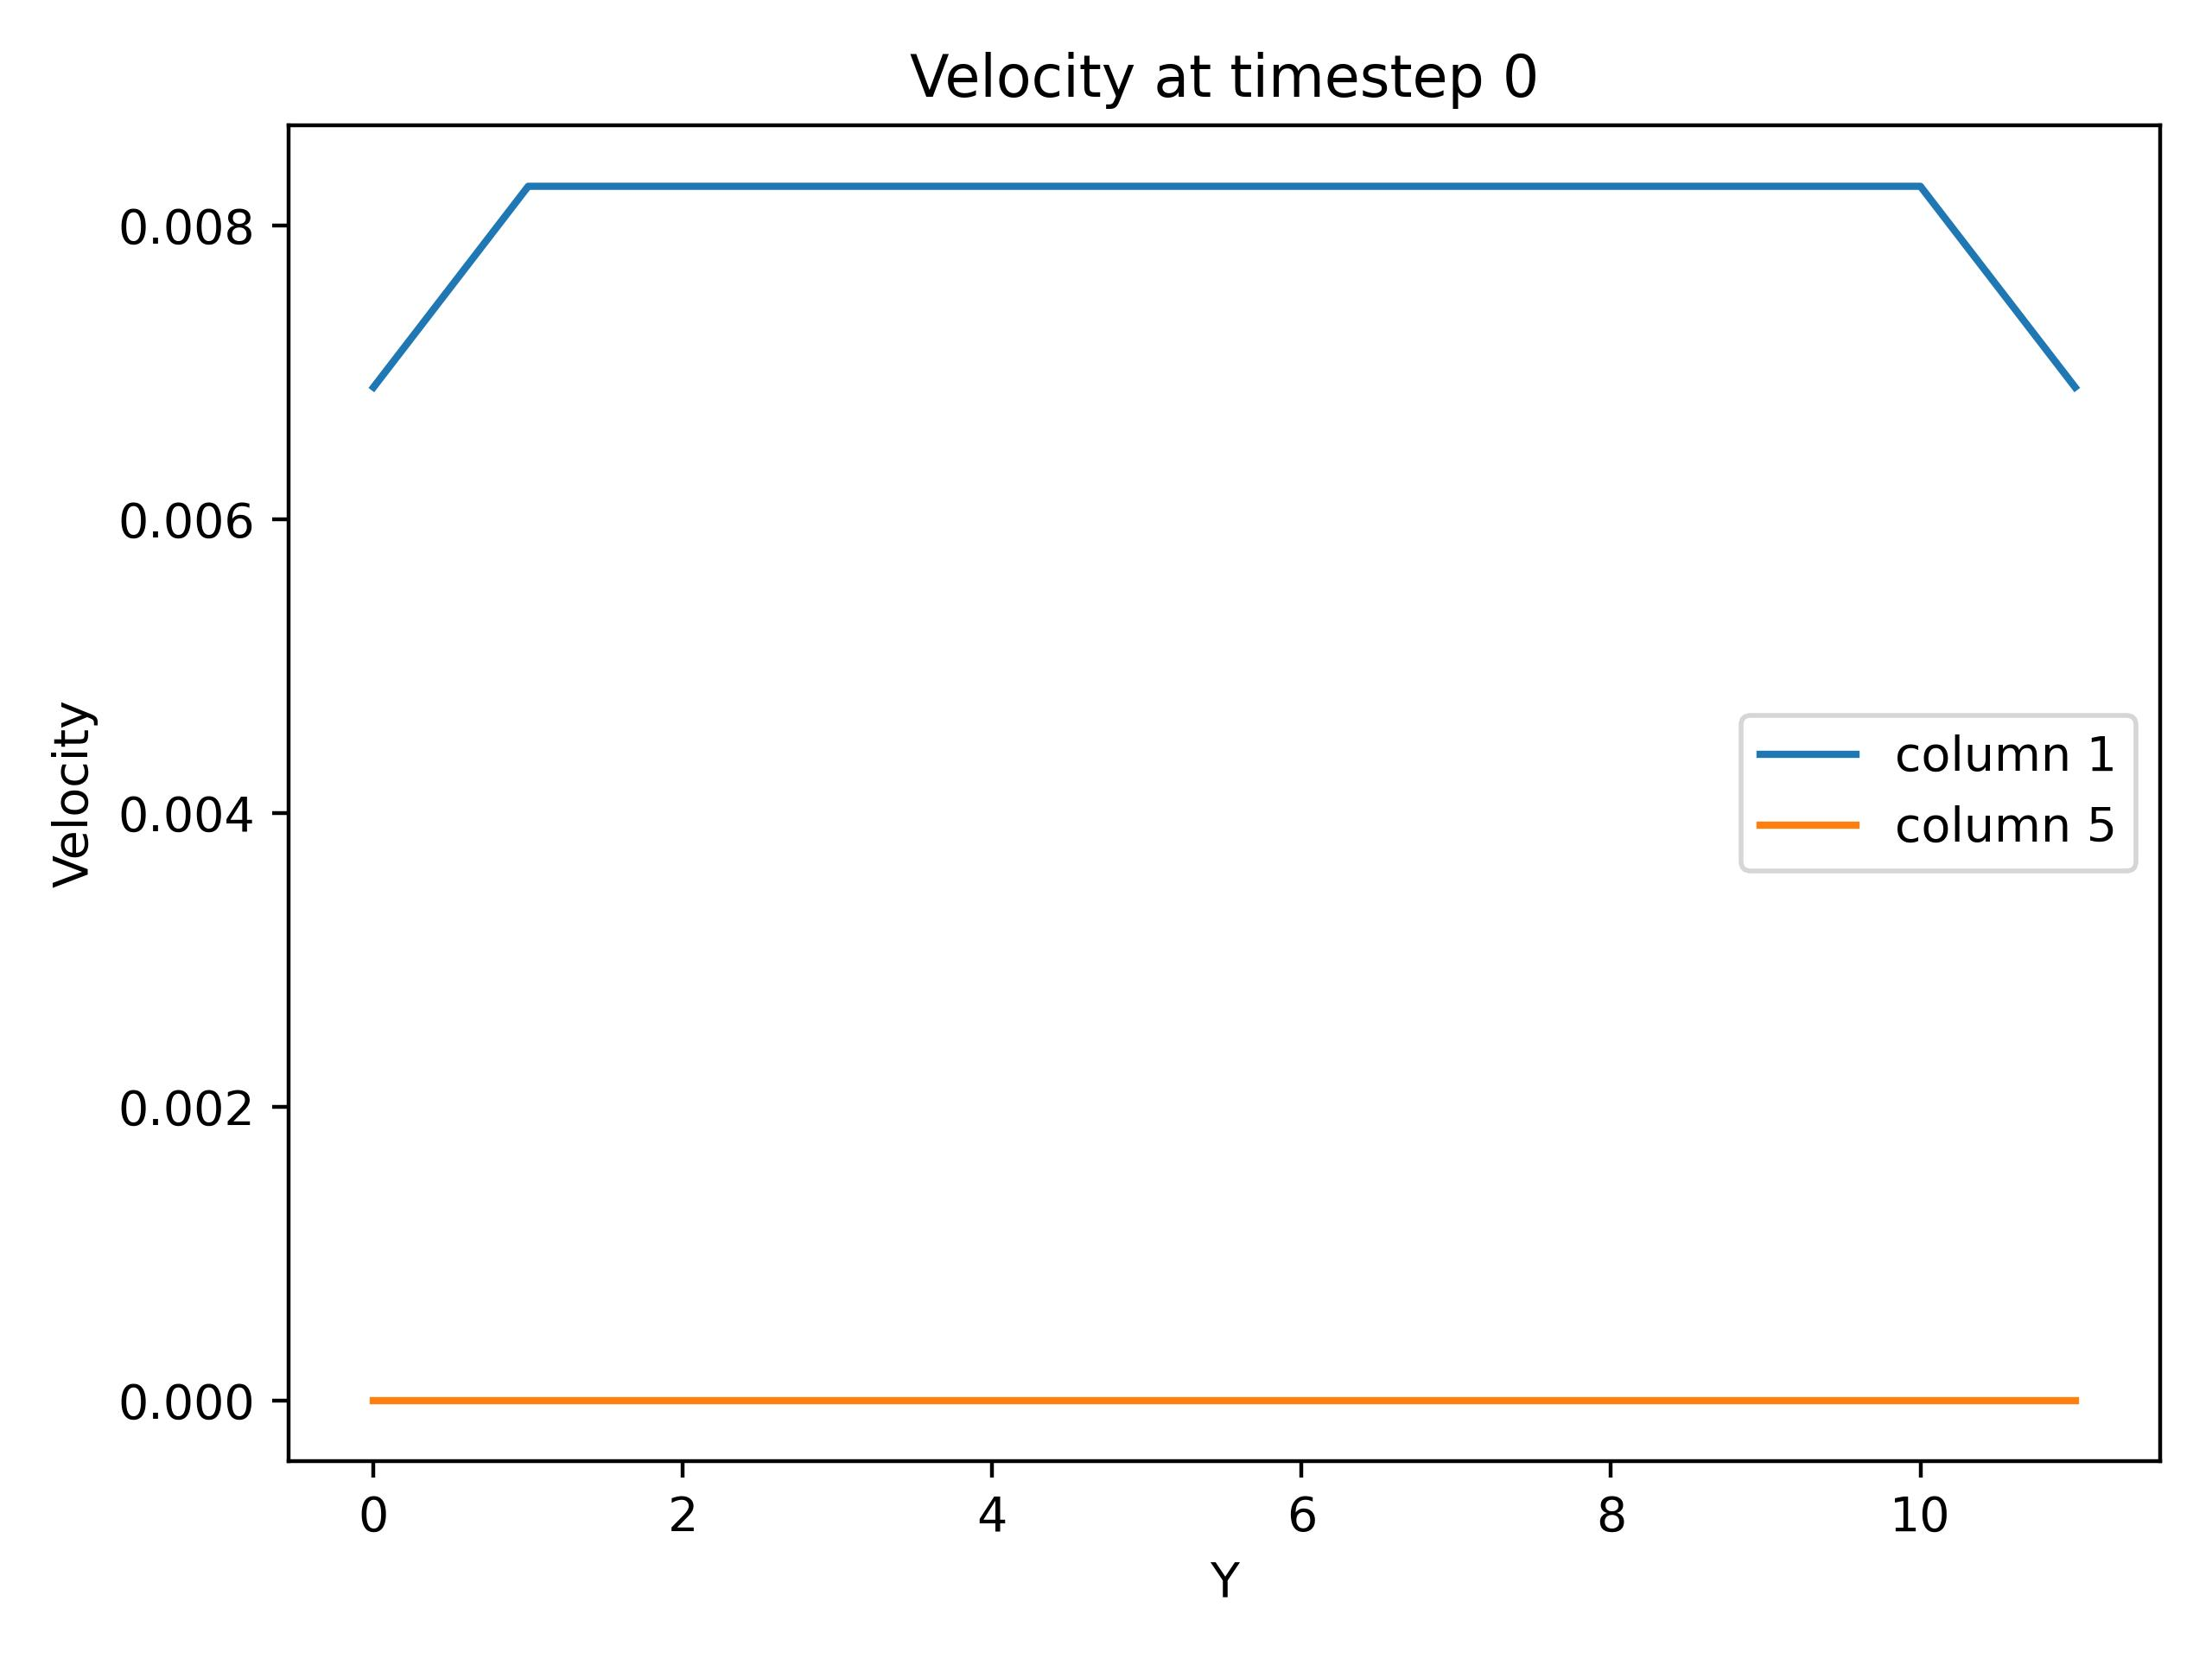
\includegraphics[width=\linewidth]{graphs/PoiseuilleFlow/velocity_at_columns_for_step_0}
    \end{minipage}% don't remove this comment - uncomments a new line
    \begin{minipage}{0.33\textwidth}
        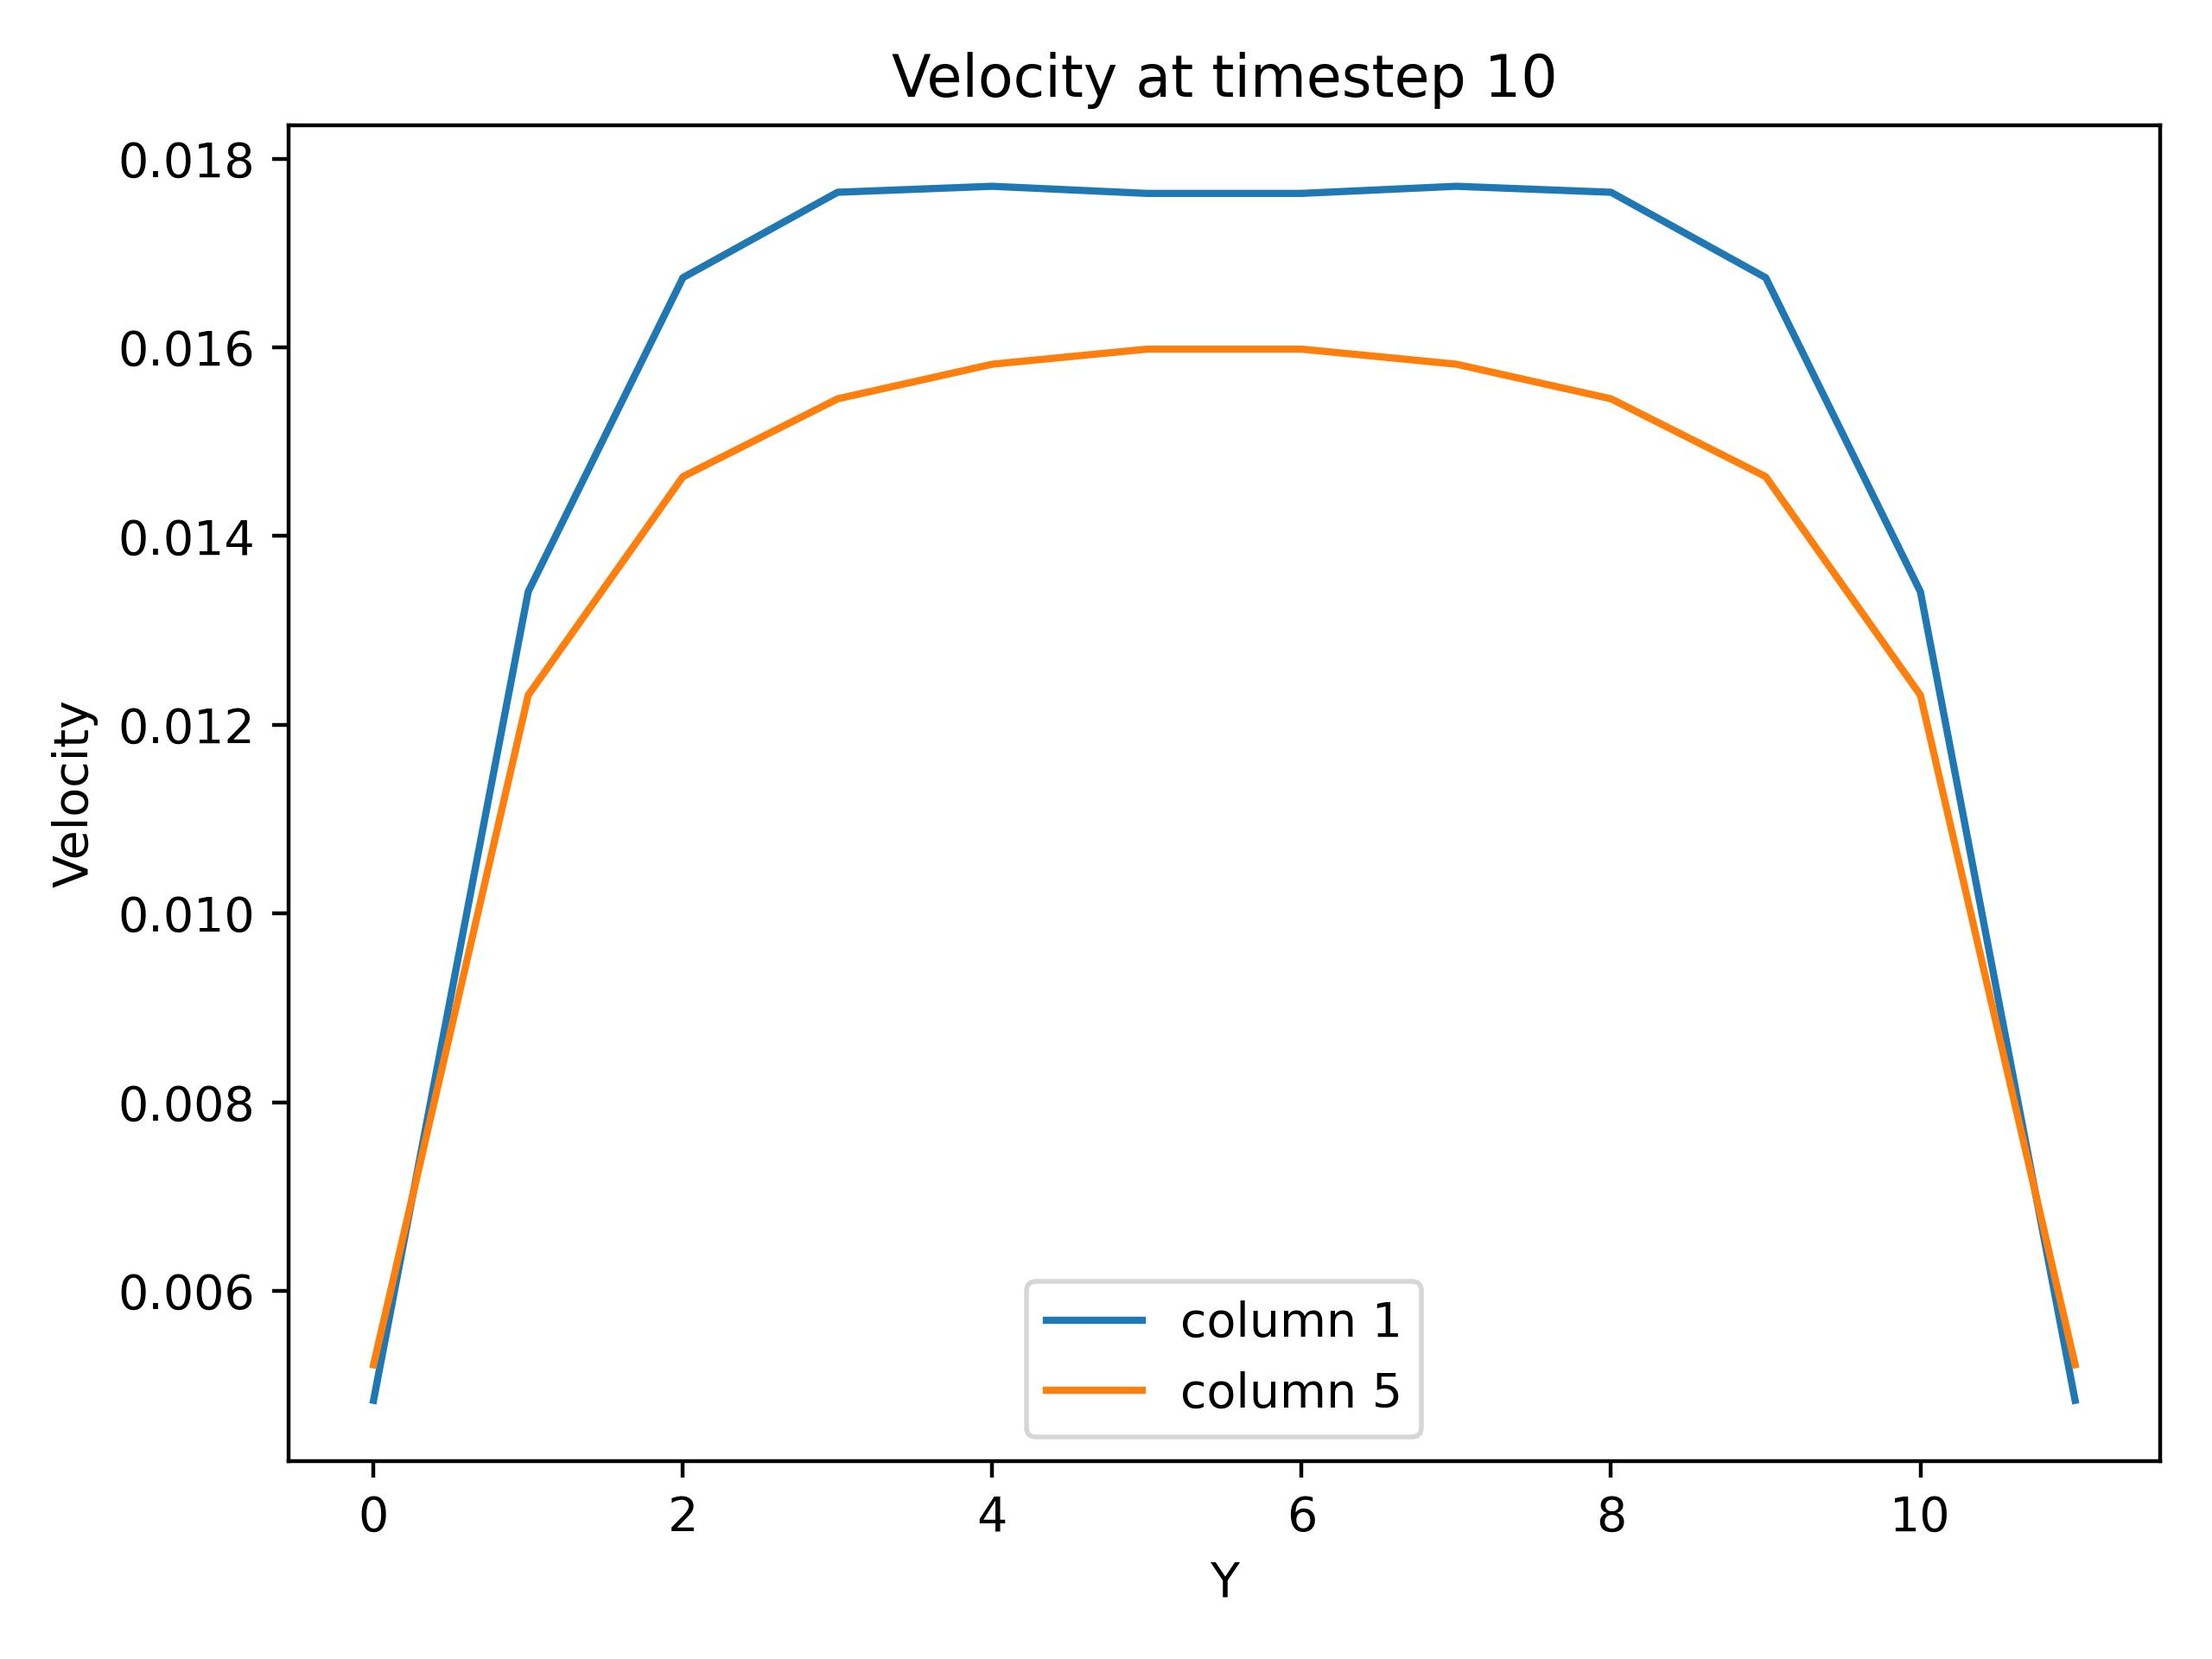
\includegraphics[width=\linewidth]{graphs/PoiseuilleFlow/velocity_at_columns_for_step_10}
    \end{minipage}% don't remove this comment - uncomments a new line
    \begin{minipage}{0.33\textwidth}
        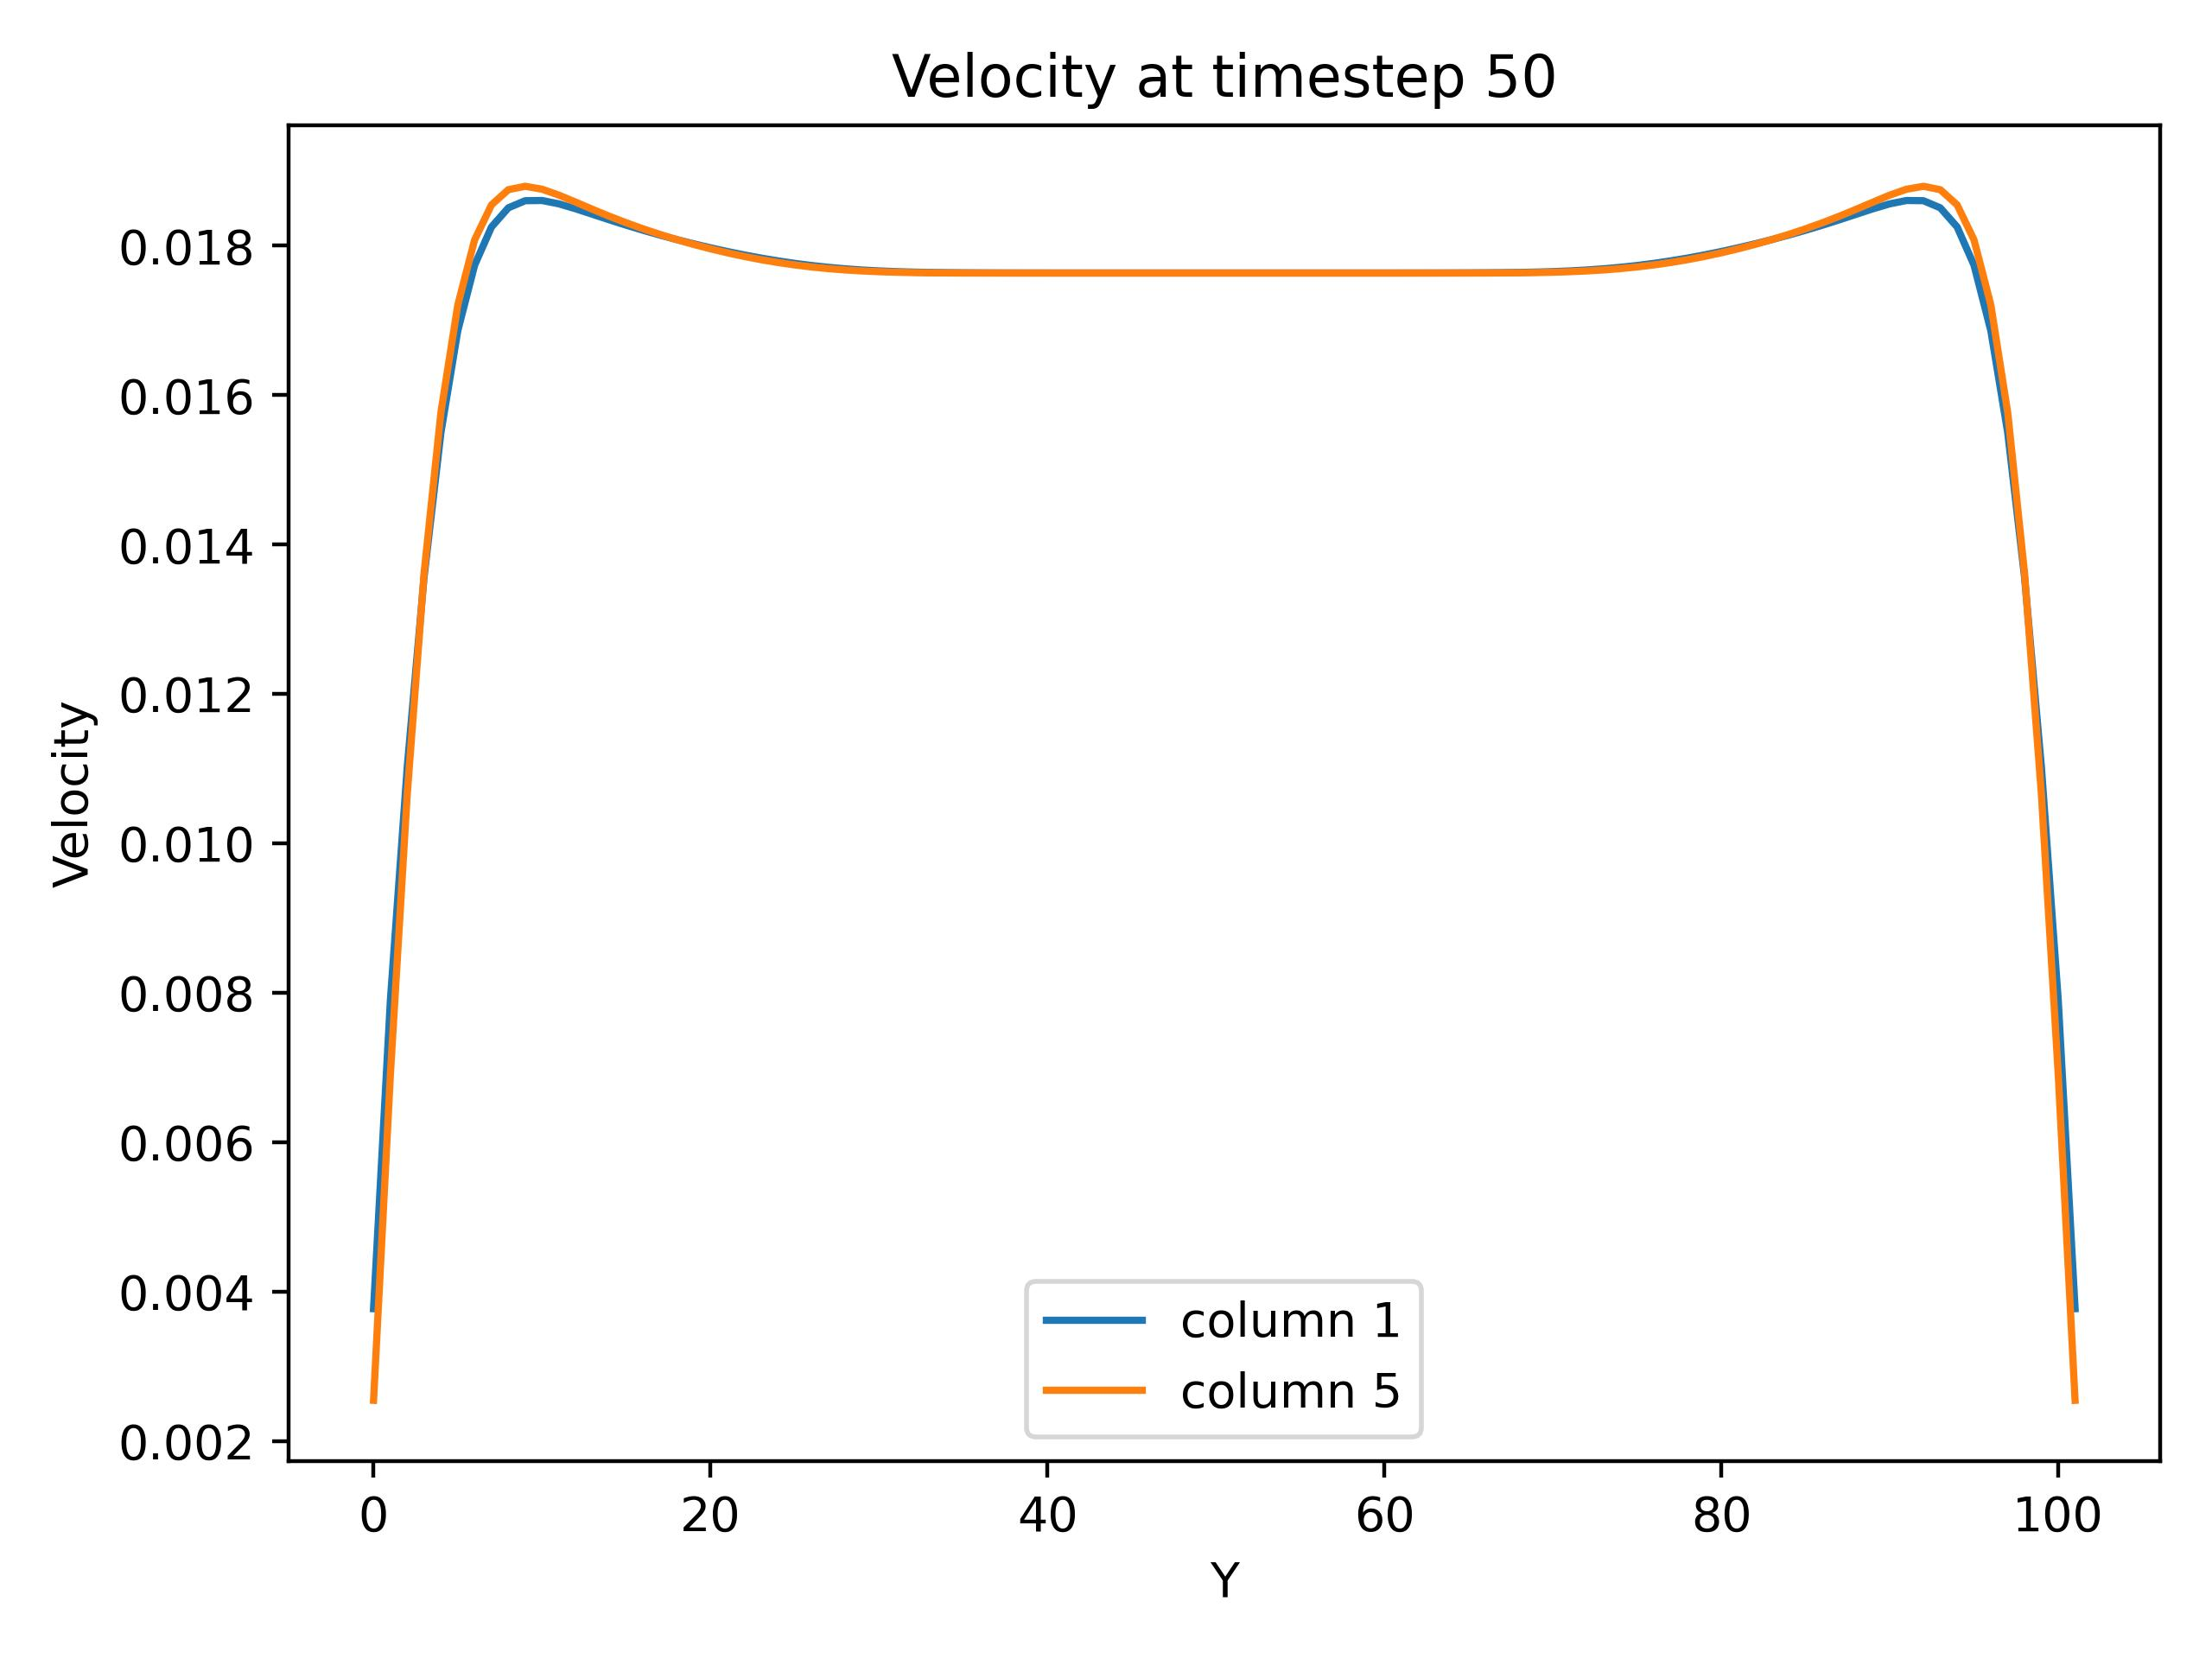
\includegraphics[width=\linewidth]{graphs/PoiseuilleFlow/velocity_at_columns_for_step_50}
    \end{minipage}
    \caption{
        Different flow states during the simulation.
    }
    \label{fig:pf-velocity-areas}
\end{figure}

The density in the center column at $\rho\left( x, \frac{L_y}{2} \right)$ is visualized in \cref{fig:pf-density}.
\begin{figure}[h!]
    \begin{center}
        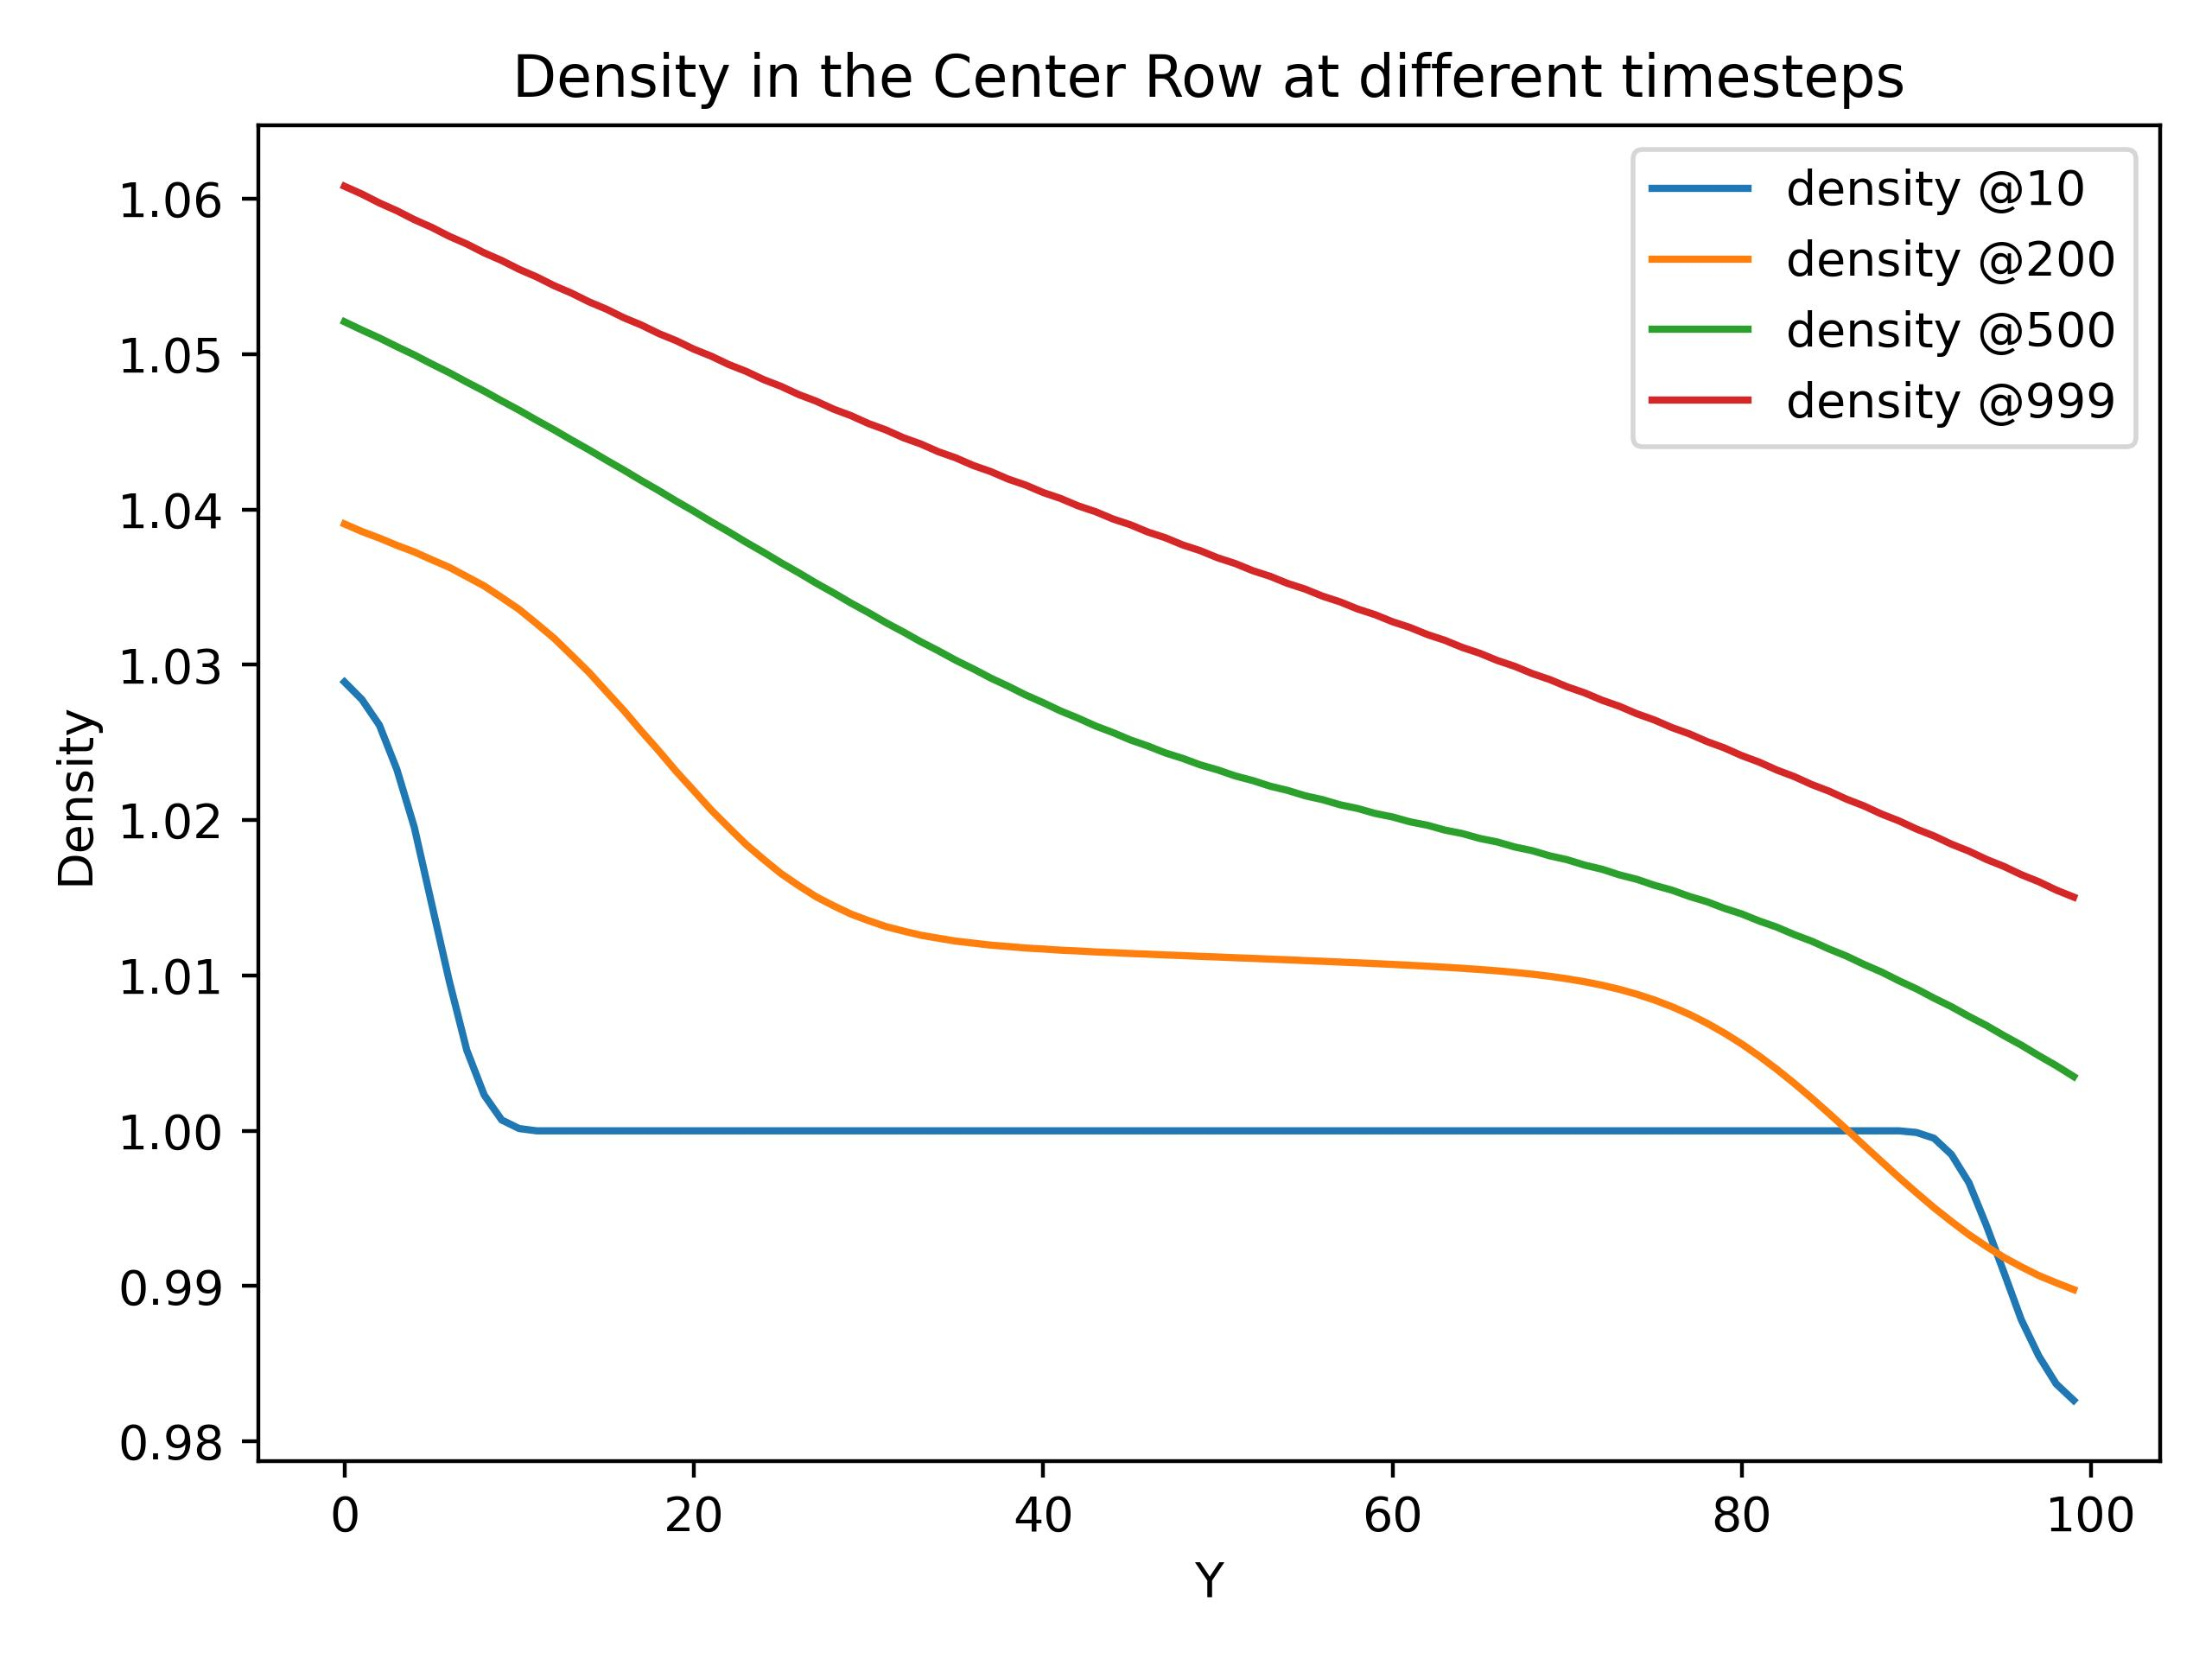
\includegraphics[width=0.5\linewidth]{graphs/PoiseuilleFlow/density_at_column_x}
        \caption{Density along the center of the Pipe.}
        \label{fig:pf-density}
    \end{center}
\end{figure}


    \chapter{Conclusion}\label{ch:conclusion}
In this project several experiments were successfully run.
This includes the \textit{Shear Wave Decay} of \cref{sec:shear-wave-decay} with 2 different initial conditions.
In addition, the correlation between viscosity and $\omega$ was measured.

Furthermore, the \textit{Couette Flow} and \textit{Poiseulle Flow} were run.
Both experiments showcased, how fluid behaves with different outer boundaries.
While the \textit{Couette Flow} showed the behavior of a sliding lit with static ground in \cref{sec:couette-flow}, the \textit{Poiseulle Flow} introduces pressure to bring movement into a fluid in a pipe in \cref{sec:poiseuille-flow}.
Both experiments showed especially the effects of friction to the movement of the fluid.

Finall the \textit{Sliding Lit} experiment combined elements of the previous experiments to simulate a fluid in a box with a sliding lit.
The project was further parallelized as shown in \cref{sec:parallelization}.
The parallelization showed a decreasing effectiveness with the number of processes in \cref{sec:sliding-lit}, which is explainable by the communication overhead.
\newline

Overall the experiments were quite successfull, there were only minor problems.
One of them was the datatype of the probability density function.
The type was in the beginning only float32, which led to unstable behavior with increasing runtime of the experiment.
\newline

The project in general is written in a very extensable manner with a focus on clean code.
Therefore it could be extended in the future.
Another experiment, that could be conducted, would be the introduction of an obstacle in the center of the simulation.
This leads to different streams around the obstacle, depending on its shape.



    \chapter{Chapter 1}

    This is an example of a citation \cite{timm2016lattice}.
    The corresponding paper can be found in the bibliography section at the end of this document.

    Lorem ipsum dolor sit amet, consectetur adipiscing elit.
    Duis risus ante, auctor et pulvinar non, posuere ac lacus. Praesent egestas nisi id metus rhoncus ac lobortis sem hendrerit. Etiam et sapien eget lectus interdum posuere sit amet ac urna.

    Example of normal equation
    \begin{equation}
        \label{eq:LBE}
        f_i(\mathbf{x}_j+\mathbf{c}_i\cdot\Delta t,t+\Delta t)=f_i(\mathbf{x}_j,t)
        -\omega \left( f_i(\mathbf{x}_j,t)-f_i^\text{eq}(\mathbf{x}_j,t) \right)
    \end{equation}

    Example of aligned equation:
    \begin{align}
        \rho(\mathbf{x}_j, t) &= \sum_i f_i(\mathbf{x}_j, t) \\
        \mathbf{u}(\mathbf{x}_j, t) &= \frac{1}{ \rho(\mathbf{x}_j, t)}
        \sum_i \mathbf{c}_i f_i(\mathbf{x}_j, t)
    \end{align}


    \section{section title}
    Lorem ipsum dolor sit amet, consectetur adipiscing elit. Duis risus ante, auctor et pulvinar non, posuere ac lacus. Praesent egestas nisi id metus rhoncus ac lobortis sem hendrerit. Etiam et sapien eget lectus interdum posuere sit amet ac urna. Aliquam pellentesque imperdiet erat, eget consectetur felis malesuada quis. Pellentesque sollicitudin, odio sed dapibus eleifend, magna sem luctus turpis.

    \begin{itemize}
        \item Example of a list
        \item Example of a list
        \item Example of a list
    \end{itemize}


    \chapter{Chapter 2}

    \begin{figure}[H]
        \begin{center}
            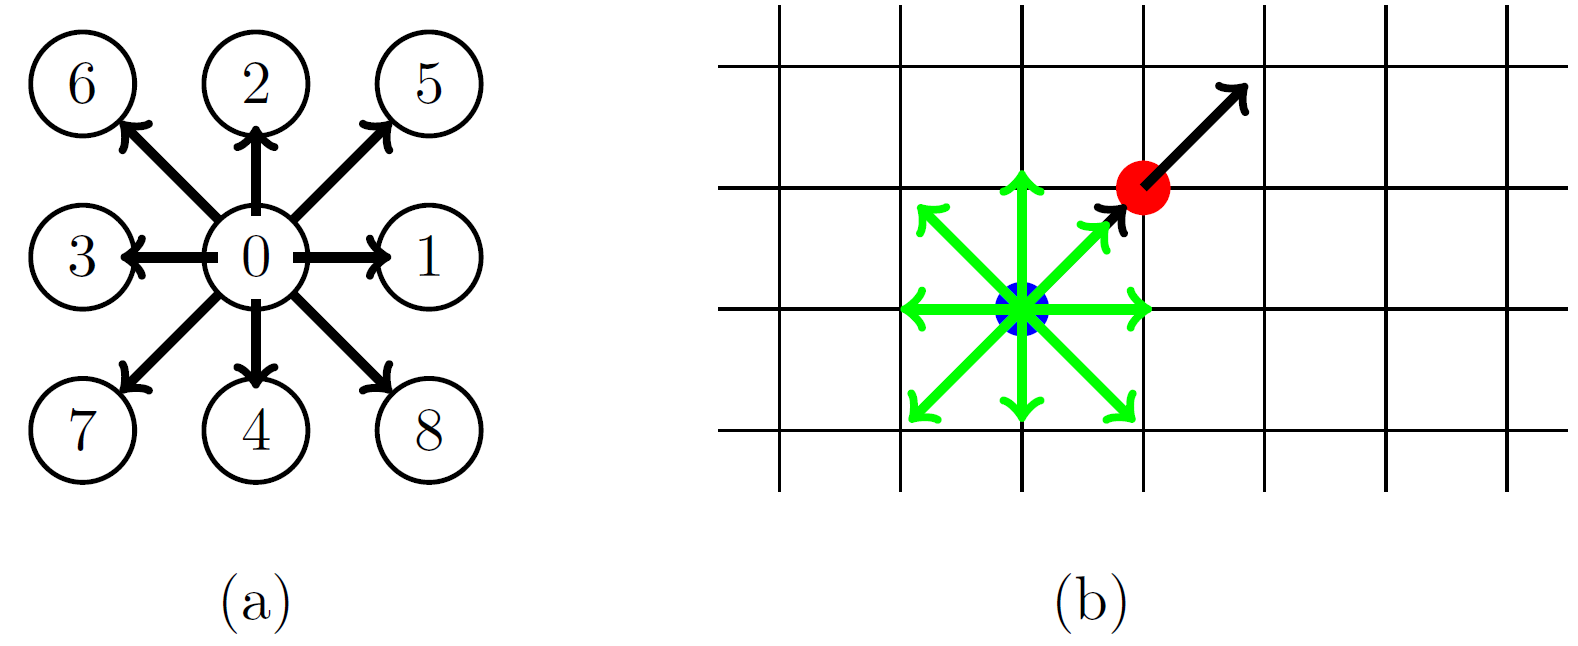
\includegraphics[width=10cm]{logos/Gitter_LBM.png}
            \caption{example figure}
            \label{fig:mesh}
        \end{center}
    \end{figure}


    \section{Section title}
    Lorem ipsum dolor sit amet, consectetur adipisicing elit, sed do eiusmod tempor incididunt ut labore et dolore magna aliqua. Ut enim ad minim veniam, quis nostrud exercitation ullamco laboris nisi ut aliquip ex ea commodo consequat. \\ Duis aute irure dolor in reprehenderit in voluptate velit esse cillum dolore eu fugiat nulla pariatur. Excepteur sint occaecat cupidatat non proident, sunt in culpa qui officia deserunt mollit anim id est laborum.
    id convallis magna eros nec metus. Sed vel ligula justo, sit amet vestibulum dolor. Sed vitae augue sit amet magna ullamcorper suscipit. Quisque dictum ipsum a sapien egestas facilisis.

    \begin{table}[ht]
        \caption{Sample table} % title of Table
        \centering % used for centering table
        \begin{tabular}{c c c c}
% centered columns (4 columns)
            \hline\hline %inserts double horizontal lines
            S. No. & Column\#1 & Column\#2 & Column\#3 \\ [0.5ex]
% inserts table
%heading
            \hline % inserts single horizontal line
            1      & 50        & 837       & 970       \\
            2      & 47        & 877       & 230       \\
            3      & 31        & 25        & 415       \\
            4      & 35        & 144       & 2356      \\
            5      & 45        & 300       & 556 \\ [1ex] % [1ex] adds vertical space
            \hline %inserts single line
        \end{tabular}
        \label{table:nonlin} % is used to refer this table in the text
    \end{table}


    \section{Code listing}

    here we provide a short example of code listing. For further information you can take look here:

    \texttt{https://www.overleaf.com/learn/latex/code\_listing}

    This is just meant to used if you think that there is some relevant part of code to be shown. Please do not append your whole implementation in the report.
    \begin{lstlisting}[language=Python]
import numpy as np
    
def incmatrix(genl1,genl2):
    m = len(genl1)
    n = len(genl2)
    M = None # to become the incidence matrix
    VT = np.zeros((n*m,1), int)  # dummy variable

    \end{lstlisting}

    \newpage

    Duis aute irure dolor in reprehenderit in voluptate velit esse cillum dolore eu fugiat nulla pariatur. Excepteur sint occaecat cupidatat non proident, sunt in culpa qui officia deserunt mollit anim id est laborum. \\ Lorem ipsum list:




    \bibliographystyle{unsrt}
    \bibliography{biblio}

\end{document}
